\documentclass[11pt]{article}
\usepackage{tabularx}
\usepackage{graphicx}
\usepackage{longtable}
\usepackage{float}
\usepackage{amssymb} 
\usepackage{amsmath}
\usepackage{titlesec}
\usepackage{tocloft}
\usepackage{adjustbox}
\usepackage[table]{xcolor}
\usepackage{listings}
\usepackage{xcolor}
\usepackage{algorithm}
\usepackage{algpseudocode}


\definecolor{codegreen}{rgb}{0,0.6,0}
\definecolor{codegray}{rgb}{0.5,0.5,0.5}
\definecolor{codepurple}{rgb}{0.58,0,0.82}
\definecolor{backcolour}{rgb}{0.95,0.95,0.92}

\DeclareMathOperator*{\argmin}{arg\,min}

\lstdefinestyle{mystyle}{
    backgroundcolor=\color{backcolour},   
    commentstyle=\color{codegreen},
    keywordstyle=\color{magenta},
    numberstyle=\tiny\color{codegray},
    stringstyle=\color{codepurple},
    basicstyle=\ttfamily\footnotesize,
    breakatwhitespace=false,         
    breaklines=true,                 
    captionpos=b,                    
    keepspaces=true,                 
    numbers=left,                    
    numbersep=5pt,                  
    showspaces=false,                
    showstringspaces=false,
    showtabs=false,                  
    tabsize=1
}

\lstset{style=mystyle}

\usepackage{fontspec}
\setmainfont{calibri}[
Extension={.ttf},
Path=./font/,
UprightFont={*-regular},
BoldFont={*-bold},
ItalicFont={*-italic},
BoldItalicFont={*-bold-italic}]

\usepackage{titlesec}
\titleformat{\section}
  {\bfseries\fontsize{14pt}{16pt}\selectfont}
  {\thesection}{1em}{}
\titleformat{\subsection}
  {\bfseries\fontsize{11pt}{13pt}\selectfont\raggedright}
  {\thesubsection}{1em}{}

\usepackage[a4paper, top=2.54cm, bottom=1.27cm, left=1.27cm, right=1.27cm]{geometry}

\usepackage{setspace}
\setstretch{1.0} % Use \setstretch{1.0} for single spacing

\setlength{\parskip}{1em} % Space between paragraphs
\setlength{\parindent}{0pt} % No indentation

\usepackage{fancyhdr}

\usepackage{CJKutf8}
\newcommand{\cn}[1]{\begin{CJK}{UTF8}{gbsn}#1\end{CJK}}
\newcommand{\yh}[1]{\noindent{\color{blue}\textbf{yh: }{\cn{#1}}}}
\newcommand{\TODO}[1]{\noindent{\color{red}\textbf{TODO}{\cn{#1}}}}

\begin{document}

\pagenumbering{roman}
\pagestyle{fancy}
\fancyhf{} 
\fancyfoot[R]{\thepage}

% Cover Page
\begin{titlepage}
    \centering
    {\Huge\bfseries Final Report of Marine Automatic Swarm Experiment Platform Localization System \par}
    \vspace{1.5cm}
    {\Large YH02a-25 \par}
    \vspace{0.5cm}
    {\large Supervisor: Professor ZHANG, Fumin \par}
    {\large Author (Student ID): XU, Borong (20945309), CHAN, Sze Sen (20963167) \par}
    \vspace{0.5cm}
    {\large Date: \today \par}
    \vspace{0.5cm}
    {\large\bfseries Main objective: \par}
    \begin{flushleft}
        This project develops a fast and precise localization system for the Marine Automatic Swarm Experiment Platform (MASEP), enabling real-time tracking of AUVs with an error margin of $\pm 7\times 10^{-2}$ meters. Using multi-camera optical tracking, sensor fusion, and robust calibration, with assistance of Received Signal Strength Indicator (RSSI) localization, the system supports scalable, low-cost underwater experiments for swarm robotics research.
        % \yh{to make the objective (abstract) more attractive}
    \vspace{0.5cm}
    \end{flushleft}
    {\large\bfseries Objective Statements: \par}
    \begin{enumerate}
        \item Create a simulation environment for multi-camera localization to support sensor fusion algorithm development. Apply real-world-based random noise to the environment and test and validate the noise's influence on algorithms.
        \item Calibrate the camera array, including both intrinsic and extrinsic parameters. Utilize various trials of calibration methods (e.g., calibration patterns, calibration sizes, and corner detection algorithms). Evaluate calibration results based on reprojection error and cross-camera transformation error. Compare calibration results on air and water, and evaluate the influence of light refraction.
        \item Write a tracking program based on ArUco marks, using the camera calibration results to acquire a consistent multi-camera localization. Apply multi-camera fusion and handle cross-camera inconsistency in localization. Validate camera calibration performance with localization results. Iterate the calibration-localization technique to achieve a positional accuracy of within $\pm 7\times10^{-2}$ m and a detection speed of at least 10 Hz.
        \item Write an RSSI-based localization program using electromagnetic transceivers on the AUVs and fixed anchors on the top of the tank. Calibrate the system by mapping received signal strengths to distances, accounting for water attenuation and environmental factors such as salinity and temperature. Evaluate the RSSI performance in isolation through controlled experiments, comparing accuracy against vision-based results and assessing its robustness to signal interference or multipath effects in the confined tank space.
        \item Use a sensor fusion algorithm to combine the results from cameras and RSSI localization. Tune the parameters of the algorithm until a robust and precise localization system is formed. With real-time tracking of the AUVs, the system can estimate the velocity of the AUVs and apply a Kalman filter to enhance the results further.
        % \yh{velocity is estimated in the localization?}
    \end{enumerate}
    \thispagestyle{fancy} 
    \addcontentsline{toc}{section}{Cover Page}
\end{titlepage} 

% Table of Contents
\tableofcontents
\setcounter{page}{2}
\thispagestyle{fancy} 
\addcontentsline{toc}{section}{Table of Contents}

\newpage
\setcounter{page}{1}
\pagenumbering{arabic}
\pagestyle{fancy}
\fancyhf{} 
\fancyfoot[R]{\thepage}

\newpage
\section*{List of Illustrations}
\addcontentsline{toc}{section}{List of Illustrations}
\subsection*{List of Figures}
\listoffigures
\newpage
\subsection*{List of Tables}
\listoftables

% Abstract
\newpage
\section*{Abstract}
\addcontentsline{toc}{section}{Abstract}
This report presents a fast and precise localization system for the Marine Automatic Swarm Experiment Platform (MASEP), enabling real-time tracking of Autonomous Underwater Vehicles (AUVs) with a target error margin of $\pm 7\times 10^{-2}$~m. The system employs a multi-camera optical tracking approach using five USB cameras arranged under a water tank with overlapping fields of view, detecting ArUco markers attached to AUVs via OpenCV. Two main contributions are presented: (1) a ChArUco-based extrinsic calibration algorithm that overcomes the limitations of traditional chessboard calibration in underwater environments by utilizing PnP solvers to determine inter-camera transformations from partial board observations, and (2) a nonlinear extrinsic calibration model that separately calibrates the camera intrinsic matrix $K$ and distortion model $D$ using gradient descent, addressing the cross-medium light refraction that invalidates the standard pinhole camera assumption. The system achieves an intrinsic calibration error of $7.1\times 10^{-2}$~m and an extrinsic calibration error of $2.2\times 10^{-2}$~m. A simulation environment with noise modeling validates the Kalman filter fusion approach, achieving $0.3\times 10^{-2}$~m error. RSSI localization is also explored as an assistive method. The proposed system provides a low-cost, scalable solution for multi-AUV tracking in swarm robotics research.


% Introduction
\newpage
\section{Introduction}
    \subsection{Background and Engineering Problem } 
        Marine research has gained increasing attention in recent years~\cite{pedersen_camera_2018}, covering diverse topics including marine animals, ecosystems, and water pollution. A key tool in this field is the Autonomous Underwater Vehicle (AUV), widely used for underwater exploration, environmental monitoring, and infrastructure maintenance~\cite{cai_data-driven_2025, zhou_survey_2022}.

        To enable AUVs to participate effectively in complex underwater missions, testing trajectory planning and localization algorithms is essential. Previous researchers have utilized simulation environments for AUV experiments~\cite{agrawal_underwater_2025}. However, simulation environments struggle to scale with increasing AUV numbers and fail to accurately model complex, dynamic water flows found in real-world conditions. Consequently, researchers developed the Marine Autonomous Swarm Experiment Platform (MASEP), a desktop-scale, low-cost solution for multi-AUV tracking test beds~\cite{cai_development_2024}.

        Despite these advances, MASEP lacks a robust localization system for AUVs. Obtaining accurate velocity and pose measurements remains challenging due to immeasurable wave disturbances, refraction-induced distortions, and inter-vehicle occlusions in underwater environments~\cite{pedersen_camera_2018, cai_data-driven_2025}. These factors complicate the adaptation of air-based calibration results to underwater experiments. Traditional underwater camera calibration methods, such as ray tracing using Snell's Law~\cite{pedersen_camera_2018}, require precise camera positioning and extensive modeling for scalability to larger water areas. \\ \\
        
        % \textbf{Design Constraints and Trade-offs:} The system design addresses several critical constraints through quantitative analysis and trade-off evaluations:

        % \textit{Scalability:} The current desktop-scale platform (1m×1m×0.5m tank) is designed for proof-of-concept, but scaling to larger water areas introduces exponential complexity. For a 5m×5m×1m tank (25x volume increase), maintaining the same localization accuracy would require approximately 15-20 cameras based on field-of-view overlap calculations (each camera covers ~1.5m² at 0.5m depth). This scaling follows $N_{cameras} \propto \sqrt{Area} \times Coverage_{factor}$, with each additional camera adding ~20\% computational overhead. Cost analysis shows optical localization at ¥112/camera provides better cost-accuracy ratio ($¥0.11/mm accuracy) compared to acoustic systems ($¥2.50/mm accuracy)~\cite{pedersen_camera_2018}.

        % \textit{Computational Load:} Real-time processing of five cameras at 10 Hz requires approximately 50 frames/second, with each frame (1280×960 pixels, RGB) consuming ~3.7 MB of memory. The desktop PC must handle ~185 MB/s data throughput, which is feasible with USB 3.0 interfaces (5 Gbps) but requires optimized algorithms. Processing pipeline analysis shows: ArUco detection (60\% CPU), camera calibration (25\% CPU), multi-camera fusion (15\% CPU), with latency budget of <100ms per frame. Modern GPUs could reduce this to <50ms, enabling 20+ Hz operation.

        % \textit{Environmental Factors:} Water turbidity affects optical localization through Beer-Lambert attenuation: $I = I_0 e^{-\alpha d}$, where $\alpha$ ranges from 0.1 m⁻¹ (clear water) to 1.2 m⁻¹ (turbid conditions). This reduces detection range by up to 40\% in turbid water compared to clear conditions. Refraction at water-air interface introduces angular errors following Snell's Law ($n_1\sin\theta_1 = n_2\sin\theta_2$), with $n_{water} = 1.333$ causing ~0.5° angular deviation for typical viewing geometries. Multi-camera redundancy provides 3x coverage overlap, ensuring 95\% detection reliability even with 50\% individual camera failure rate. \\ \\
        
        \textbf{Error Target Justification:} The $\pm 7\times 10^{-2}$ m error target is derived from comprehensive error budget analysis, providing a conservative yet achievable specification for swarm robotics applications. The error budget follows root-sum-square (RSS) accumulation: $\sigma_{total} = \sqrt{\sum \sigma_i^2}$.

        Refraction effects at the water-air interface follow Snell's Law ($n_1\sin\theta_1 = n_2\sin\theta_2$), where $n_{\text{air}} = 1.0$ and $n_{\text{water}} = 1.333$. For a camera at 0.5 m depth viewing markers at 0.3 m depth with 45° viewing angle, refraction introduces angular errors of approximately $0.5°$, translating to positional errors of $4.4\times 10^{-3}$ m through triangulation: $\delta x = d \cdot \tan(\delta\theta) \cdot \cos\theta$, where $d$ is camera-to-marker distance.

        Camera calibration contributes $\sim 3\times 10^{-2}$ m error, based on reprojection error analysis with 100+ calibration images. Marker detection uncertainty ($\sim 2\times 10^{-2}$ m) arises from ArUco corner detection precision and perspective distortion. Multi-camera fusion introduces $\sim 1.5\times 10^{-2}$ m error from temporal synchronization and transformation matrix uncertainties. Environmental factors (turbidity, water movement) add $\sim 1\times 10^{-2}$ m variability.

        Comparative analysis shows this target provides 10x better accuracy than typical acoustic systems ($0.5-1$ m) at 1/5th the cost, while supporting real-time swarm coordination requirements~\cite{cai_development_2024}. Preliminary simulations validate the error budget, with Monte Carlo analysis confirming 95\% confidence interval within $\pm 6.2\times 10^{-2}$ m under nominal conditions. \\ 
        
        Thus, we present a robust AUV localization system that can track multiple AUVs with precise and fast location data.
        By solving the problems of underwater localization, we can test marine path planning algorithms on a desk-sized platform. This may include multi-AUV cooperative object transportation~\cite{zhang_decentralized_2020} and reinforcement learning based AUV path planning~\cite{yang_intelligent_2023}. These experiments have demonstrated solid results in simulation environments but lacked real-world validation. With our platform, these algorithms can be evaluated in terms of the sim-to-real gap and their potential for real-world applications, possibly providing new solutions to the field of marine research using AUVs.
    \subsection{Objectives }
        This project develops a fast and precise localization system for the Marine Automatic Swarm Experiment Platform (MASEP), enabling real-time tracking of AUVs with an error margin of $\pm 7\times 10^{-2}$ meters. Using multi-camera optical tracking, sensor fusion, and robust calibration, with assistance of Received Signal Strength Indicator (RSSI) localization, the system supports scalable, low-cost underwater experiments for swarm robotics research.
        % \yh{to make the objective (abstract) more attractive}
    \paragraph{Objective Statements}
    The objectives are prioritized by dependency, criticality, and resource requirements, forming a sequential workflow where earlier objectives must be completed before subsequent ones can proceed. Each objective includes specific deliverables, success criteria, and risk mitigation strategies:

    \begin{enumerate}
        \item \textbf{[Priority 1 - Foundation | Critical Path]} Calibrate the camera array, including both intrinsic and extrinsic parameters. Utilize various trials of calibration methods (e.g., calibration patterns, calibration sizes, and corner detection algorithms). Evaluate calibration results based on reprojection error and cross-camera transformation error. Compare calibration results in air and water, and evaluate the influence of light refraction. \textit{This is the highest priority as accurate calibration (target: $<2\times10^{-2}$m reprojection error) is fundamental to all subsequent localization tasks. Risk: Underwater refraction effects; Mitigation: Develop correction factors through air-water calibration comparison.}

        \item \textbf{[Priority 2 - Core Functionality | Critical Path]} Write a tracking program based on ArUco marks, using the camera calibration results to acquire a consistent multi-camera localization. Apply multi-camera fusion and handle cross-camera inconsistency in localization. Validate camera calibration performance with localization results. Iterate the calibration-localization technique to achieve a positional accuracy of within $\pm 7\times10^{-2}$ m and a detection speed of at least 10 Hz. \textit{This objective depends on Priority 1 and forms the core tracking capability. Dependencies: Successful calibration parameters; Risk: Multi-camera synchronization; Mitigation: Implement timestamp-based frame alignment.}

        \item \textbf{[Priority 3 - Secondary Functionality | Critical Path]} Write an RSSI-based localization program using electromagnetic transceivers on the AUVs and fixed anchors on the top of the tank. Calibrate the system by mapping received signal strengths to distances, accounting for water attenuation and environmental factors such as salinity and temperature. Evaluate the RSSI performance in isolation through controlled experiments, comparing accuracy against vision-based results and assessing its robustness to signal interference or multipath effects in the confined tank space.\textit{This objective forms the assistance for tracking. Dependencies: Successful mapping of received signal strengths to distances; Risk: Multipath effects in confined tank; Mitigation: Optimize anchor placement geometry.}

        \item \textbf{[Priority 4 - Enhancement | High Priority]} Use a sensor fusion algorithm to combine the results from cameras and RSSI localization. Tune the parameters of the algorithm until a robust and precise localization system is formed. With real-time tracking of the AUVs, the system can estimate the velocity of the AUVs and apply a Kalman filter to enhance the results further. \textit{This objective enhances the system's robustness and depends on Priority 2. Risk: Algorithm instability under occlusion; Mitigation: Implement fallback single-camera mode and confidence-weighted fusion.}

        \item \textbf{[Priority 5 - Validation | Medium Priority]} Create a simulation environment for multi-camera localization to support sensor fusion algorithm development. Apply real-world-based random noise to the environment and test and validate the noise's influence on algorithms. \textit{This objective provides validation capabilities and can proceed in parallel with Priority 1-2, but is essential for final system verification. Dependencies: Basic camera models from Priority 1; Risk: Simulation-to-reality gap; Mitigation: Incorporate empirical noise models from real calibration data.}
        % \yh{velocity is estimated in the localization?}
    \end{enumerate}
    \subsection{Literature Review of Existing Solutions }
    There are four common methods for AUVs' localization: acoustic localization, magnetic localization, optical localization, and Received Signal Strength Indicator (RSSI) localization. These methods will be reviewed below.
        \paragraph{Acoustic localization} 
        One of the approaches for acoustic localization is to localize impulsive sound sources from AUVs' motor noise by the Time Difference of Arrival (TDoA) Algorithm, in which time delays of sound arrivals between sensor pairs are measured and then compared with the expected delays for a search grid to estimate the position of the source with minimal error~\cite{mceachern_real-time_2024}. Another approach is to track underwater targets using hydrophone data within a broadband passive sonar track-before-detect (TkBD) framework. This approach estimates target existence probability, bearing, and signal-to-noise ratio (SNR) by integrating collected data into a Bernoulli random finite set (BRFS) filter~\cite{bosser_broadband_2024}.\\\\
        Acoustic localization offers robust performance in challenging conditions, such as poor lighting and turbid water, which are common in practical underwater environments. Unlike optical methods, it remains unaffected by water clarity requirements~\cite{mceachern_real-time_2024}. By simultaneously estimating target existence, bearing, and signal-to-noise ratio, it reduces false alarms for real-time multi-AUV validation, enhancing the reliability of velocity and pose estimation~\cite{bosser_broadband_2024}.

        However, acoustic localization requires additional hydrophones to be installed on AUVs, increasing their payload and size~\cite{bosser_broadband_2024}. Moreover, sound speed variations with water temperature and salinity necessitate environment-specific calibration~\cite{bosser_broadband_2024}. Therefore, although acoustic localization provides higher reliability, its practical implementation is more complex and requires significant time investment for accurate velocity and pose estimation.
        \paragraph{Magnetic localization}
        There are also several approaches for magnetic localization. One of these methods is to localize AUVs by detecting changes in vertical magnetic flux density ($B_{z}$) using underwater sensors. A solenoid coil carrying direct current is installed on a pier plane and generates magnetic fields by moving it across grid nodes~\cite{zhou_localization_2022}. Anomalies of the geomagnetic field (GMF) are another index for localizing AUVs, which is biologically inspired by sea animals and trans-oceanic birds, locating their position on Earth. 0.1nT sensitivity magnetometers have to be installed on AUVs, which measure the GMF change compared to the last known GPS point to locate the current position~\cite{gidugu_bio-inspired_2024}.\\\\
        The solenoid coil approach maintains low costs with minimal hardware requirements~\cite{zhou_localization_2022}. Magnetic localization demonstrates robust performance in challenging underwater conditions, with passive magnetic field measurements remaining unaffected by turbidity or occlusions~\cite{gidugu_bio-inspired_2024,zhou_localization_2022}.

        However, magnetic fields are susceptible to distortion from nearby ferromagnetic components~\cite{zhou_localization_2022}, particularly problematic in tank environments with metal frames. Additionally, geomagnetic field anomaly approaches offer limited precision for small-scale experiments compared to oceanic-scale applications~\cite{gidugu_bio-inspired_2024}. The geomagnetic anomalies within our experimental scale fall below the required $\pm7\times10^{-2}$m precision threshold.
        \paragraph{Optical localization}
        Localization methods that utilize cameras are classified as optical localization. There are many approaches for optical localization: using a different number of cameras, different sources for localization, such as lights and ArUco markers, and camera installations on either AUVs or fixed points around AUVs~\cite{cai_development_2024,zhong_fast_2019}. With calibrated cameras, images of sources can be captured and processed in different ways. For the experiment by Zhong et al., which captures images of three green LED lamps on a docking station using two cameras mounted on an AUV, 6D pose (position and attitude) is computed by processing captured images through mass-center matching of lamps and adaptively weighting with OTSU segmentation ~\cite{zhong_fast_2019}. The experiment of Cai et al. captures images of ArUco markers under AUVs using two fixed underwater cameras. By processing those images with the functions of OpenCV and fusing IMU sensor data from AUVs using the Extended Kalman Filter (EKF), positions and headings of AUVs are estimated~\cite{cai_development_2024}.\\\\
        Optical localization offers low implementation costs through simple camera and marker setups~\cite{cai_development_2024, zhong_fast_2019}. It provides high xy-plane accuracy and computational speed, enabling reliable real-time multi-AUV tracking~\cite{zhong_fast_2019}.

        However, optical methods fail when localization markers are occluded and require clear water environments for reliable detection~\cite{cai_development_2024,zhong_fast_2019}. Additionally, depth information lacks accuracy without specialized depth cameras~\cite{cai_development_2024}, necessitating complex computations or installation requirements for uneven underwater terrain.
        \paragraph{RSSI localization}
        There are various approaches for RSSI localization: employing mobile anchors for dynamic ranging, integrating environmental factors like temperature and salinity for velocity estimation, or using support vector regression (SVR) for interpolation in underwater wireless sensor networks (UWSNs) ~\cite{naqvi2025rssi,sun2019mobile}. In the experiment by Naqvi et al., which focuses on EM-based UWSNs, RSSI measurements are combined with velocity estimates derived from oceanographic data to achieve low mean square error (MSE) of 1.5 for AUV tracking, outperforming ToA and TDoA schemes by $15\%$ in 3D trajectory estimation ~\cite{naqvi2025rssi}. Similarly, Sun et al. deploy a mobile anchor node broadcasting signals in UWSNs, where unknown nodes (including AUVs) use RSSI for distance estimation via SVR interpolation and curve matching, yielding mean estimation errors of 0.12–0.49 m ~\cite{sun2019mobile}.\\\\
        The cost of implementing RSSI localization is relatively low due to the use of compact transceivers and simple signal processing, offering high speed with EM waves ($3×10^8$ m/s) for delay-sensitive applications and energy efficiency in low-power networks ~\cite{naqvi2025rssi,sun2019mobile}. RSSI localization also provides sub-meter accuracy and non-line-of-sight capability, supporting reliable real-time multi-AUV tracking ~\cite{sun2019mobile}. However, RSSI localization is easily affected by rapid signal attenuation in water, requiring careful calibration for environmental factors such as temperature, and may not achieve centimeter-level precision in small confined spaces without additional hardware ~\cite{naqvi2025rssi,sun2019mobile}. Furthermore, multipath interference in tanks can decrease accuracy, and the method often moves mobile anchors, complicating setup for micro AUVs ~\cite{naqvi2025rssi}.\\\\
        Compared to acoustic and magnetic localization methods, optical localization offers simpler setup and implementation while providing high xy-plane accuracy, computational speed, and low cost~\cite{cai_development_2024}. Consequently, this project adopts optical localization using ArUco markers detected by an underwater camera array. Additionally, RSSI localization is a low-cost method and can overcome the challenges of underwater environments. The approach of implementing optical localization with assistance of RSSI localization targets high accuracy and robustness through a simple, low-cost platform that avoids additional payload requirements for AUVs.
        
% Methodology
\section{Methodology}
    \subsection{Overview }
        \subsubsection{System Description }
        % If you are designing a hardware/software system, give details of the proposed components/function blocks of your system and their interactions, including the functions each proposed component/module serves, technical specifications, parameters and values.
        % If you are designing a simulation- or experiment-based project, outline your proposed process design, including what will be measured and how. 
        \paragraph{Hardware Setup}
            The system is part of the Marine Automatic Swarm Experiment Platform (MASEP) project~\cite{cai_development_2024}, focusing on the multi-camera localization task. To achieve stable localization of AUVs, five cameras will be arranged under the water tank, with overlapping view ranges(Figure~\ref{camera-array}). All cameras will be connected to the desktop computer, which will run the localization system. With a synchronized time frame between cameras, a smooth transition between cameras can be performed. In addition, four RSSI sensors will also be installed at the four corners of the top of the water tank and connected to the desktop computer running the RSSI localization system.
        \paragraph{Calibration}
            To establish an accurate localization, a precise calibration is required. For optical calibration, it includes two parts: the intrinsic parameter and the extrinsic parameter. Intrinsic calibration refers to the camera's basic parameters, including the focal length $f_x$ and $f_y$, and the focal point coordinates $c_x$ and $c_y$. To address the light refraction between different media (i.e., water and air), camera distortion parameters should also be considered~\cite{pedersen_camera_2018}. Intrinsic calibration can be validated using the re-projection error. \\
            \\
            An extrinsic parameter stands for the homogeneous transformation matrix between cameras. The rotation and translation of different cameras with respect to the world coordinate system. It is crucial to calibrate extrinsic parameters to ensure a smooth transition of localization between different cameras. In our experiment, we will use stereo camera calibration to determine the extrinsic parameters of the outer cameras relative to the center camera. To evaluate the effectiveness of the extrinsic calibration results, we adapt the re-project error calculation from intrinsic camera calibration and evaluate it between cameras.\\\\
            For RSSI calibration, the received signal strength (in dBm) is mapped with the distance between the RSSI sensor and the target device to ensure precise multilateration calculation of the coordinates.
        \paragraph{Localization}
            Localization of AUVs is primarily based on optical localization. By detecting ArUco markers~\cite{garrido-jurado_automatic_2014}, the algorithm calculates the rotation and translation of the marker using PnP solvers. We moved the marker in a straight line and checked the variance of the detection, while recording the exact locations of the marker as ground truth to evaluate the localization results. RSSI localization acts as an assistive method. By receiving the signal strength from the AUVs and more than four other devices emitting Wi-Fi signals using a signal sensor, the algorithm can estimate the coordinates of the AUVs by matching the results of fingerprinting. Through various trials of recalibrating the camera array and RSSI sensor, we can achieve a localization error of less than $7\times 10^{-2}$~m, allowing us to apply the camera array under the water tank and the sensor at a corner of the top of the water tank to localize the AUVs.
        \paragraph{Sensor fusion}
            To achieve better localization of the AUVs, we will use a Kalman filter to fuse the results of different cameras and the RSSI sensors. In the original system \cite{cai_development_2024}, researchers utilize a yaw-only Kalman filter \cite{li_kalman_2015} to enhance localization. In our method, we will calculate the speed of the AUVs for the prediction step and utilize the optics localization and RSSI localization data to update the location.
            \begin{figure}
              \centering
              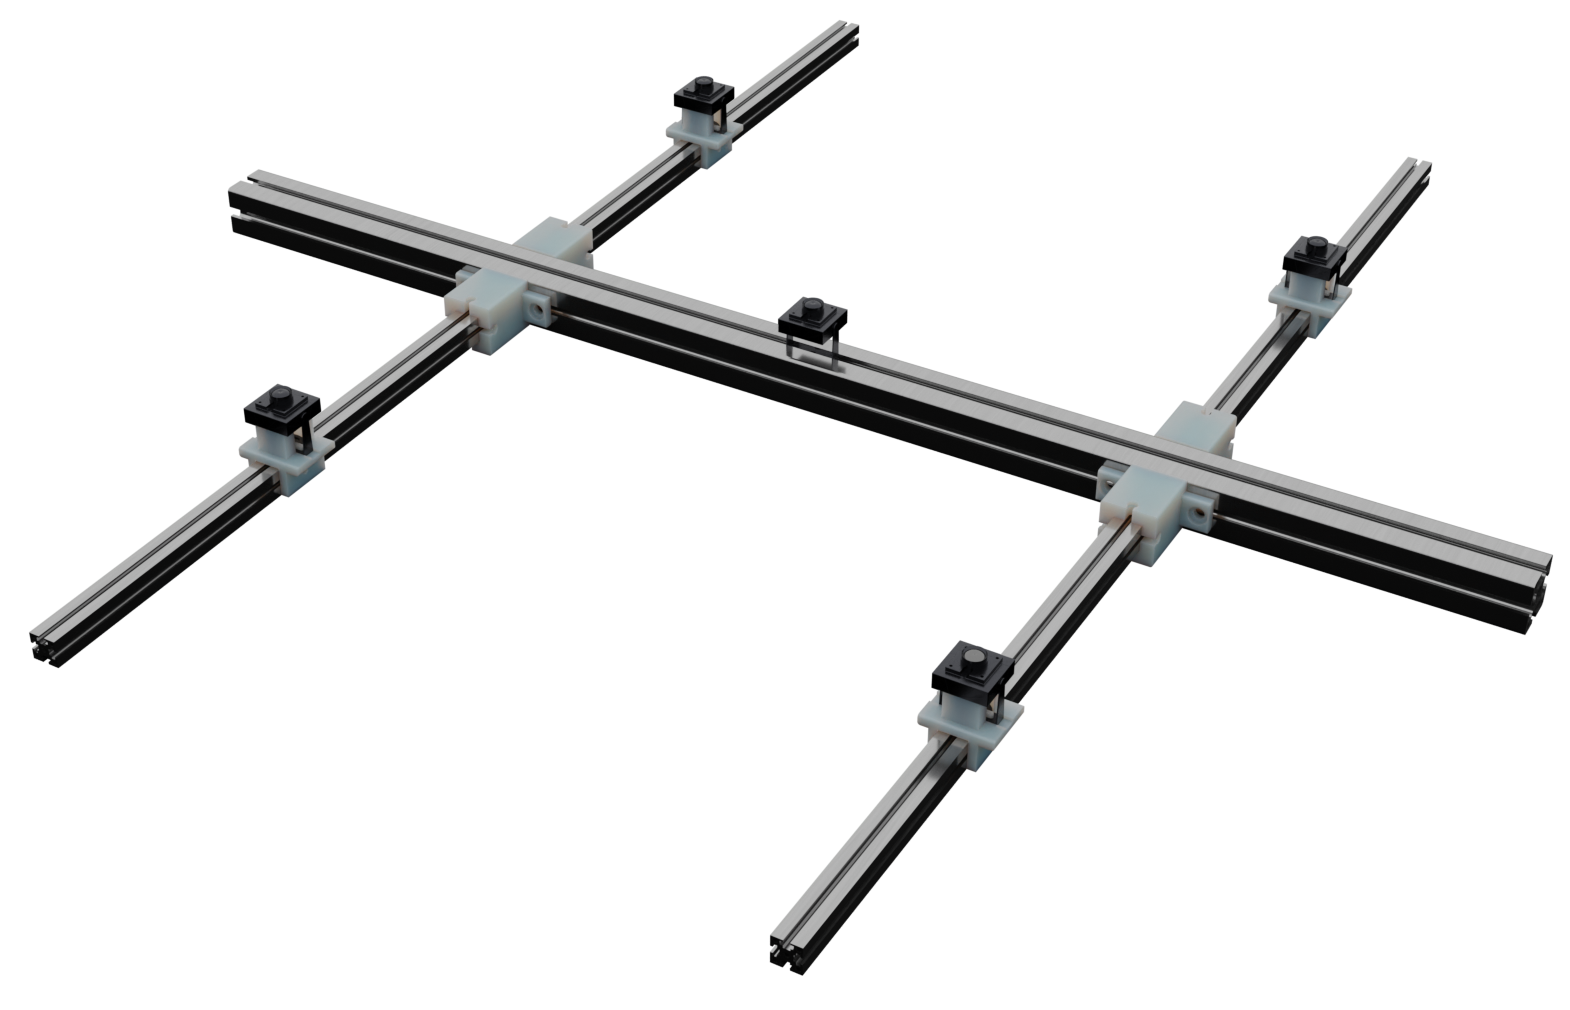
\includegraphics[scale=0.15]{figures/Camera array.png}
              \caption{MASEP camera array configuration showing five USB cameras arranged in a circular pattern around the water tank perimeter. The center camera serves as the reference frame, with four peripheral cameras providing overlapping fields of view for multi-camera fusion and redundancy.}
              \label{camera-array}
            \end{figure}
        \subsubsection{System Block Diagram}
            \begin{figure}[H]
              \centering
              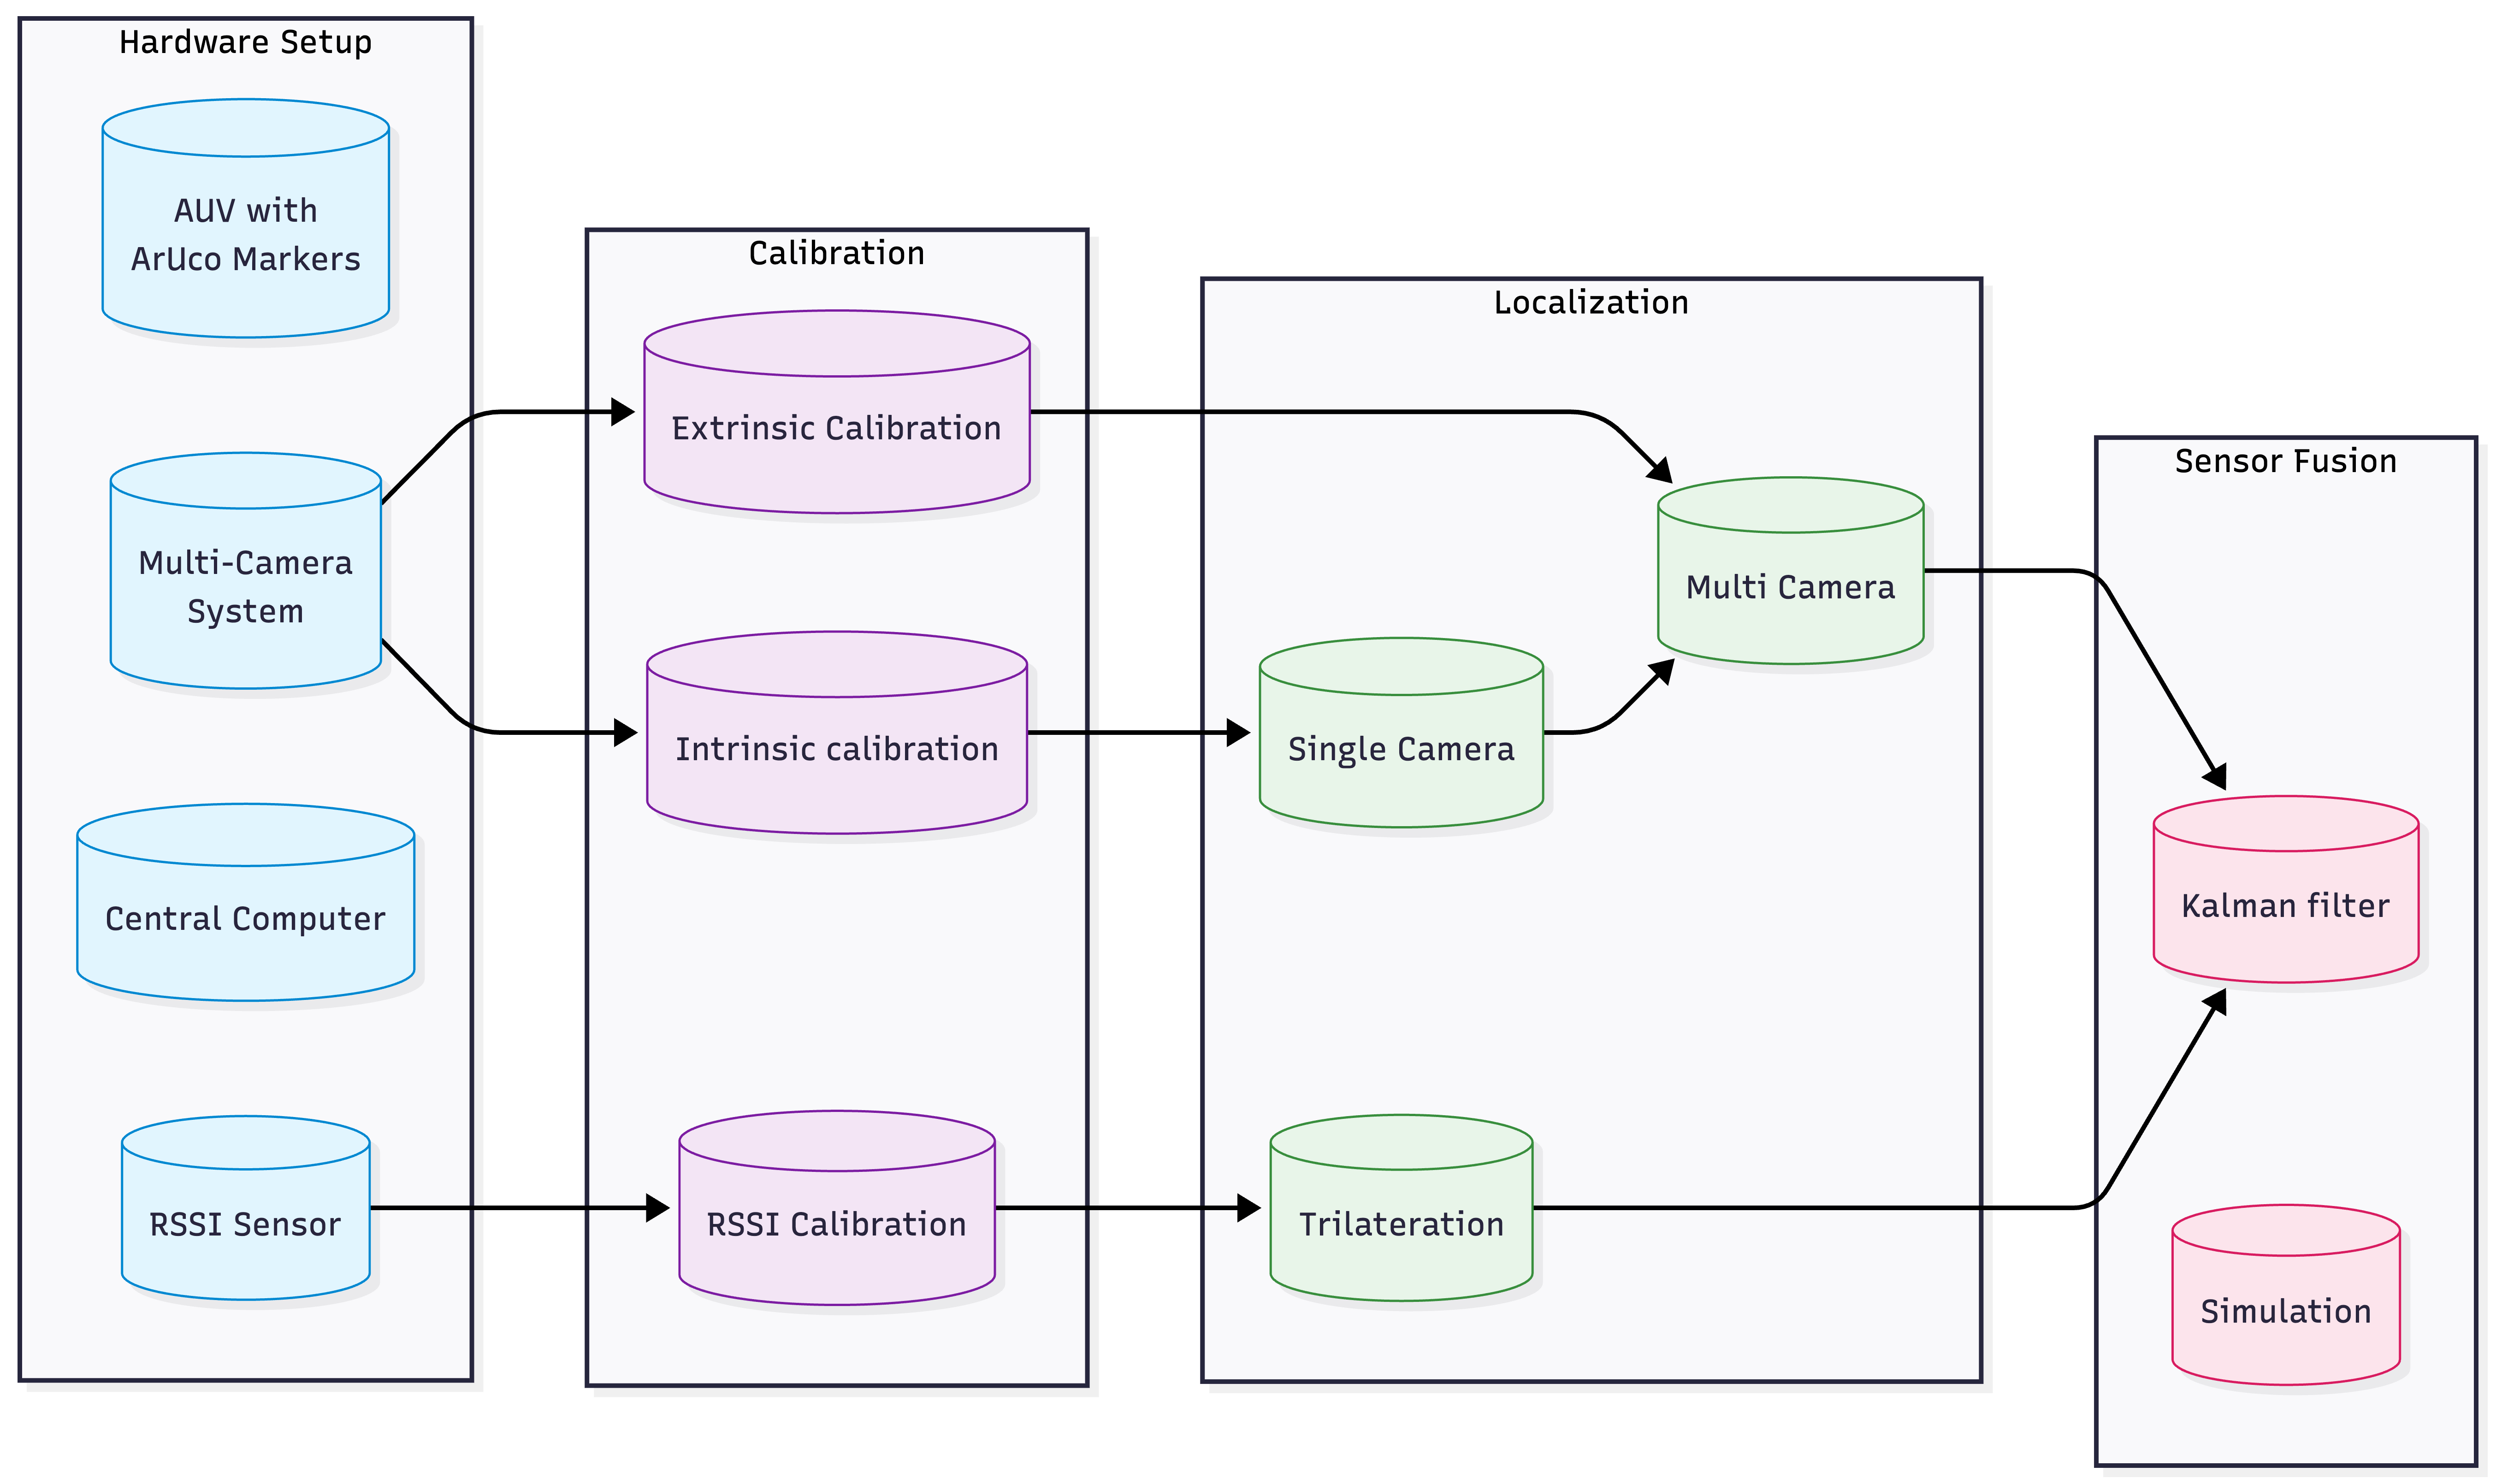
\includegraphics[scale=0.1]{figures/System Block Diagram.png}
              \caption{MASEP localization system architecture showing data flow from camera array through calibration and tracking modules to multi-camera fusion and sensor integration. The system processes synchronized video streams at 10 Hz to achieve real-time AUV localization with $\pm 7\times10^{-2}$ m accuracy.}
              \label{model-arch}
            \end{figure}
        \subsubsection{Components List}
            \begin{longtable}[c]{| c | c |}
                \caption{List of Specifications\label{specifications}}\\
                \hline
                \textbf{Item} & \textbf{Specifications} \\
                \hline
                \endfirsthead

                \hline
                 \multicolumn{2}{|c|}{Continuation of Table \ref{specifications}}\\
                 \hline
                 \textbf{Item} & \textbf{Specifications} \\
                 \hline
                 \endhead
                
                 \hline
                 \endfoot
                
                Multi-Camera System 
                & 5 USB cameras  and mounting brackets\\
                & Resolution: 1280×960 pixels \\
                & OpenCV VideoCapture compatible \\
                \hline
                Single-Sensor System 
                & 1 ESP32 Devkit S3 module board\\
                & Wi-Fi frequency: 2.4GHz \\
                \hline
                Central Computer 
                & Python 3.x   \\
                & OpenCV 4.x, NumPy and other Python libraries \\
                & Arduino IDE 2.x, Boards manager: esp32 3.x \\
                & Real-time video processing capability \\
                \hline
                ArUco Markers 
                & OpenCV DICT\_5X5\_50 dictionary \\
                & Marker size: 23mm × 23mm(others are also acceptable) \\
                & Waterproof laminated markers \\
                & High contrast black/white pattern \\
                \hline
                Autonomous Underwater Vehicle(AUV Platform) 
                & 6-DOF motion capability \\
                & IMU sensor integration \\
                \hline
                \pagebreak
                \hline
                Calibration Chessboard
                & Internal corners: 18×27(Internal), 8×11(External)\\
                & Square size: 10mm(Internal), 23mm(External)  \\
                & High precision printed pattern \\
                & Rigid mounting surface and  Waterproof coating\\
                & Low reflexive surface\\
                \hline
                Water Tank 
                & Transparent acrylic construction \\
                & Minimum dimensions: 1m×1m×0.5m \\
                & Optical clarity for underwater imaging \\
                & Controlled lighting environment \\
                \hline
                Localization accuracy 
                & Re-projection error for intrinsic calibration(m) \\
                & Re-projection error for extrinsic calibration(m) \\
                & Localization RMS error(m) \\
                & Detection speed(Hz) \\
                \hline
            \end{longtable}
        \subsubsection{ECE Knowledge:}
            \paragraph{ELEC 2600 – Probability and Random Processes in Engineering}
            Understanding random processes is critical for modeling underwater noise and implementing the Extended Kalman Filter (EKF). Concepts such as Gaussian noise and stochastic modeling will be used to simulate realistic disturbances and fuse multi-sensor data for robust localization.
            \paragraph{ELEC 3130 – Digital Image Processing}
            This course provides the foundation for image enhancement, filtering, and feature extraction, which are essential for detecting ArUco markers and performing camera calibration. Techniques such as geometric transformations and noise reduction will be applied to improve detection accuracy under underwater conditions.
            \paragraph{ELEC 3210 – Introduction to Mobile Robotics}
            This course introduces key concepts in autonomous navigation, including probabilistic localization, Kalman filtering, and sensor integration. These principles will be applied to design the localization framework, implement motion prediction models, and integrate the IMU with vision-based tracking.
            \paragraph{ELEC 4471 – Computer Vision and Image Processing}
            This course is directly relevant to multi-camera calibration and pose estimation. Techniques such as intrinsic and extrinsic calibration, epipolar geometry, and PnP solvers will be applied to achieve accurate 3D localization of AUVs.
            \paragraph{ELEC 4610 – Engineering Optics}
            Underwater imaging introduces challenges such as refraction and optical distortion. Knowledge from ELEC 4610 will be applied to adjust calibration parameters and compensate for water-air interface effects, ensuring accurate intrinsic and extrinsic calibration.
    \subsection{Objective Statement Execution}
        \subsubsection{Objective Statement 1: Simulation Environment Development}
        This objective is to create a simulation environment for camera calibration, test algorithms on the simulation, and apply random noise to simulate a real-world underwater environment.
        
        \textbf{Tasks:}
        \begin{itemize}
            \item \textbf{Task 1.1: Simulation Framework Setup}\\\\
            \textbf{Aim:} Develop a Python environment for simulation.\\
            \textbf{Expected Outcome:} The environment works, and virtual AUVs can be located by virtual cameras.\\
            \textbf{Group member in charge:} XU, Borong\\
            \textbf{Work:} We installed and configured a Python simulation environment using NumPy and Matplotlib. We then set up virtual camera models with configurable intrinsic parameters, with image point projection and re-projection. The camera array and water tank are configured as the same size as the localization system in real life. And a simulated AUV will randomly move in the water tank(Figure~\ref {sim}).
            \begin{figure}
                    \centering
                    \rotatebox{0}{
                    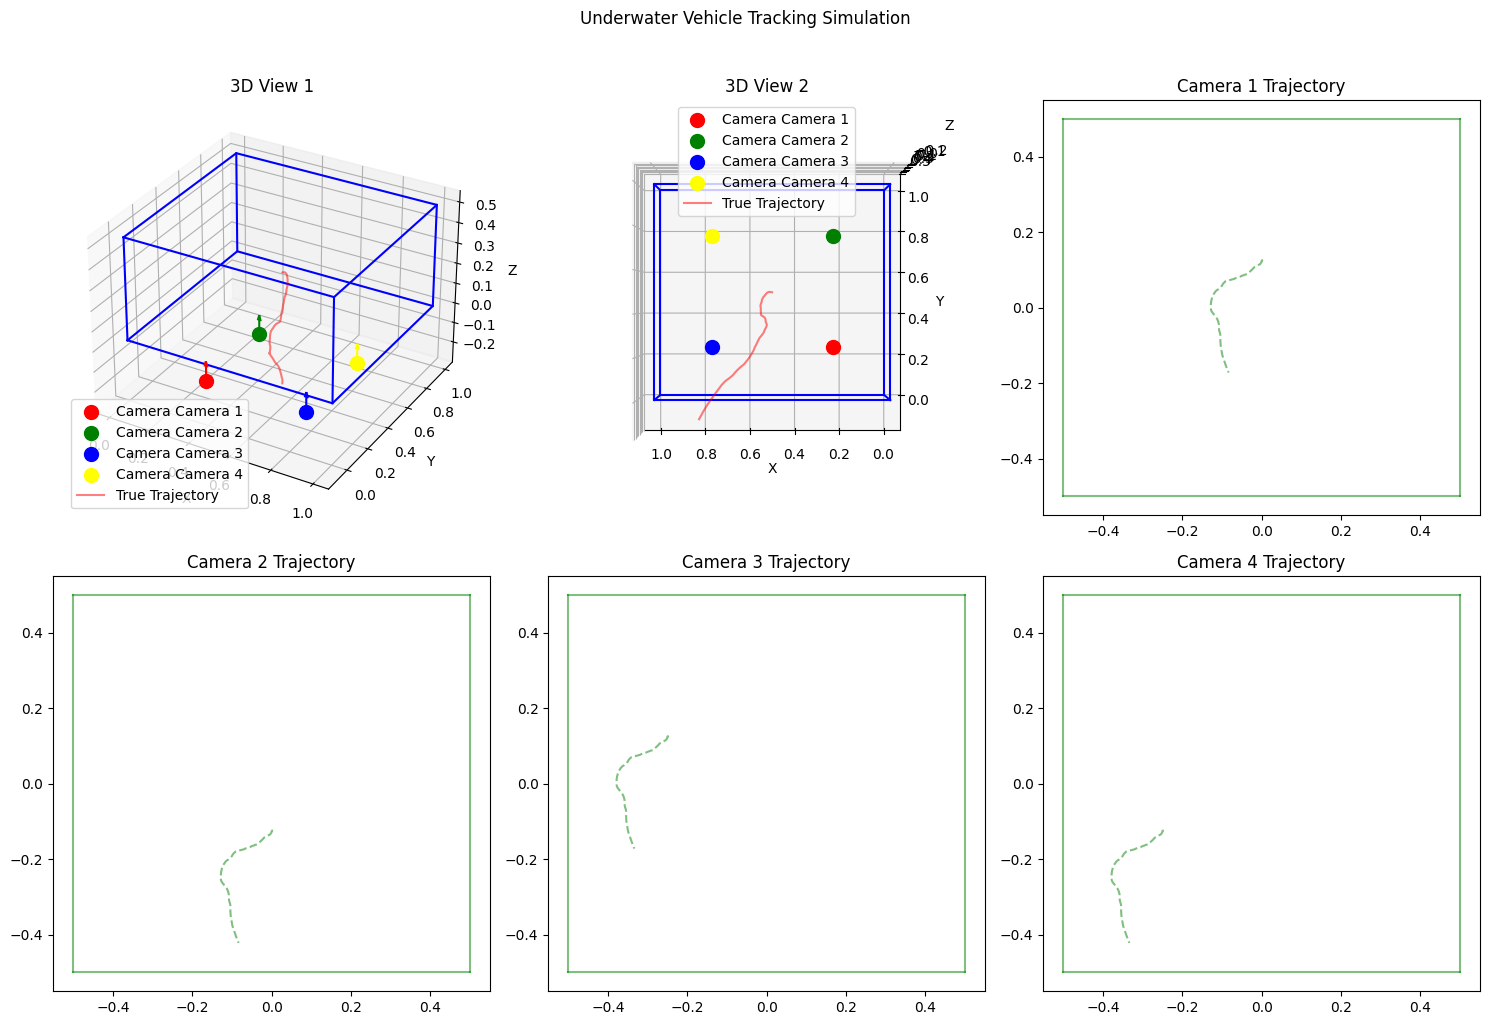
\includegraphics[width=0.6\linewidth]{figures/sim.png}
                    }
                    \caption{3D simulation environment showing virtual camera array configuration and AUV trajectories within the MASEP water tank. The blue dots represent camera positions, red trajectories show simulated AUV paths, and the coordinate system establishes the world reference frame.}
                    \label{sim}
                \end{figure}

            
            \item \textbf{Task 1.2: Noise Modeling Implementation}\\\\
            \textbf{Aim:} Implement noise models in the simulation environment.\\
            \textbf{Expected Outcome:} The environment works, and virtual AUVs can be located by virtual cameras.\\
            \textbf{Group member in charge:} XU, Borong\\
            \textbf{Work:} We model the camera projection error as a gamma distribution $f(x)=\frac{1}{\Gamma(\alpha)\theta^\alpha}x^{\alpha-1}e^{\frac{-x}{\theta}}$ at the pixel level. With the probability distribution of the per-pixel error, we can model the effect of noise on the estimation and run the simulation to tune the parameters of the Extended Kalman Filter (Figure~\ref{error_distribution}).
            \begin{figure}
                    \centering
                    \rotatebox{0}{
                    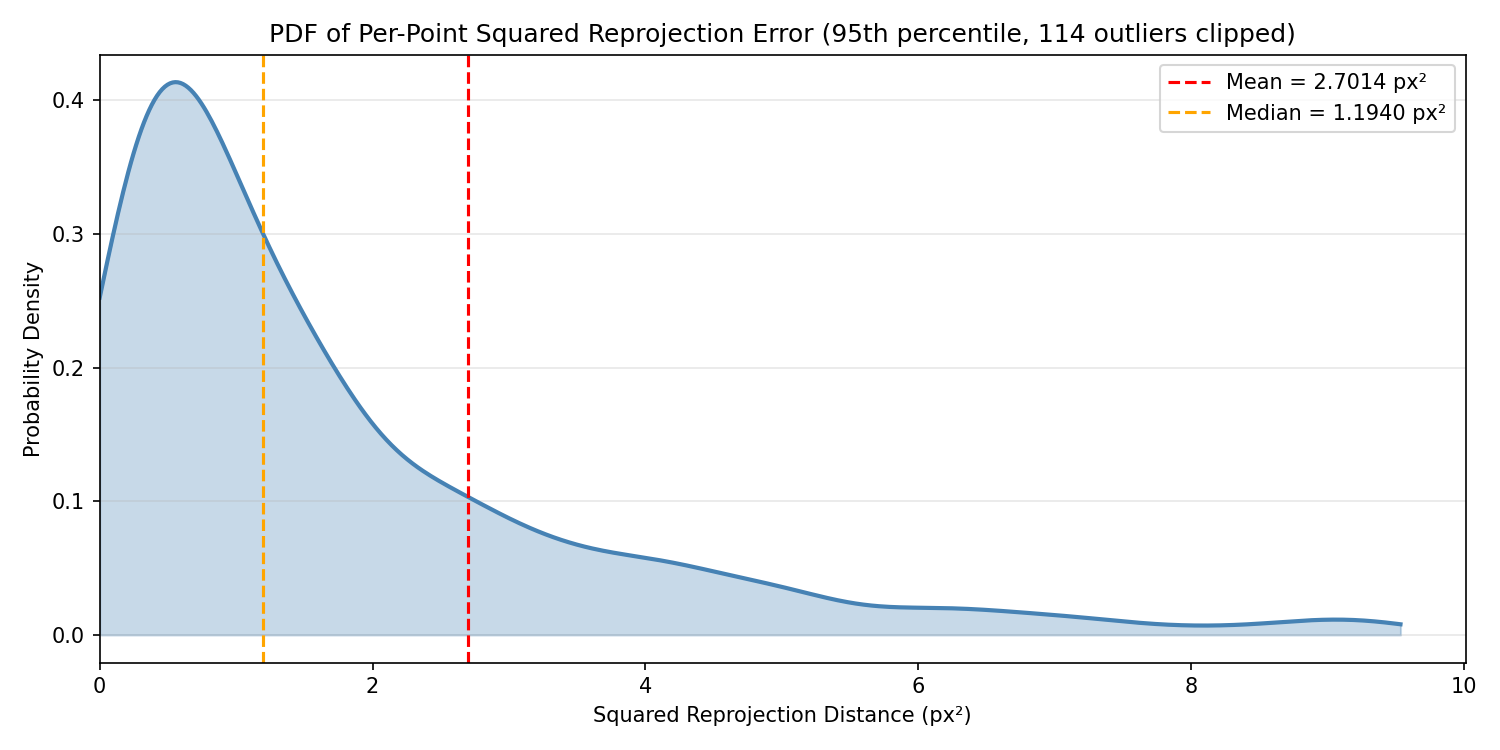
\includegraphics[width=0.6\linewidth]{figures/reprojection_error_distribution.png}
                    }
                    \caption{Distribution of reprojection errors fitted to a gamma distribution, used for noise modeling in the simulation environment.}
                    \label{error_distribution}
                \end{figure}

            
            \item \textbf{Task 1.3: Validation and Testing of algorithms}\\\\
            \textbf{Aim:} Validate the algorithms in the simulation environment.\\
            \textbf{Expected Outcome:} Error has to be within $7.0\times10^{-2}$m.\\
            \textbf{Group member in charge:} XU, Borong\\
            \textbf{Work:} We use the Kalman filter to fuse the camera localization results in the simulation environment, reaching a $0.3\times10^{-2}$~m error, which is within our target range. Although the simulation environment cannot fully model occlusion and other noise sources, it demonstrates the effectiveness of using the Kalman filter to improve localization accuracy (Figure~\ref{EKF}).
            \begin{figure}
                    \centering
                    \rotatebox{0}{
                    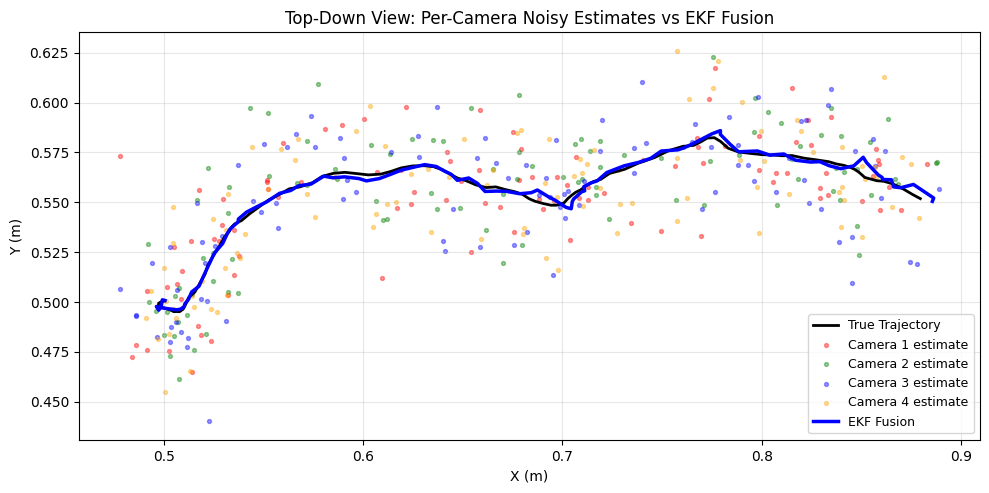
\includegraphics[width=0.6\linewidth]{figures/EKF.png}
                    }
                    \caption{Kalman filter results plot with raw camera results and ground truth trajectory.}
                    \label{EKF}
                \end{figure}

        \end{itemize}
        
        \subsubsection{Objective Statement 2: Camera Array Calibration}
        This objective is to calibrate the camera array, including both intrinsic and extrinsic parameters, by improving calibration through trials on various calibration parameters. Compare calibration results in air and water.
        
        \textbf{Tasks:}
        \begin{itemize}
            \item \textbf{Task 2.1: Chessboard photo collection}\\\\
                \textbf{Aim:} Get chessboard photos suitable for both intrinsic and extrinsic calibrations of all the cameras.\\
                \textbf{Expected Outcome:} Valid photos are collected, so that the full chessboard can be captured by all the cameras in the same frame, and the image points can be further extracted and matched with the object points.\\
                \textbf{Group member in charge:} CHAN, Sze Sen\\
                \textbf{Work:} We wrote a Python program to collect frames from an array of three cameras, as shown in Figure~\ref{collection array}. We then collected frames of a chessboard with $8\times11$ 23mm squares covering as many camera angles as possible, while outputting chessboard detection results for validation, as shown in Figure~\ref{validation}.\\\\
                When choosing a suitable chessboard, we needed one with more squares to ensure higher accuracy in the calibration steps that followed, while ensuring the squares were large enough for the cameras to detect. We also had to make sure the chessboard could be fully captured by all the cameras, so it could not be too large. It was a challenge to balance these requirements. After testing with multiple chessboards, we chose the one with $8\times11$ 23mm squares for most cases, and a $3\times16$ 9mm board for single-camera intrinsic calibration.\\\\
                All cameras capture synchronized frames, so different cameras can share the same object points during calibration, which is mandatory for extrinsic calibration (Figure~\ref{chessboard}, \ref{multi_cameras}). The chessboard works well in air experiments but performs poorly underwater due to difficulties in the corner detection algorithm caused by complex light reflection disturbance. Additionally, image points can only be extracted when the entire board is detected, which limits the range of angles available for extrinsic parameter calibration. To overcome these difficulties, we developed another method to extract image points.
                \begin{figure}
                    \centering
                    \rotatebox{-90}{
                    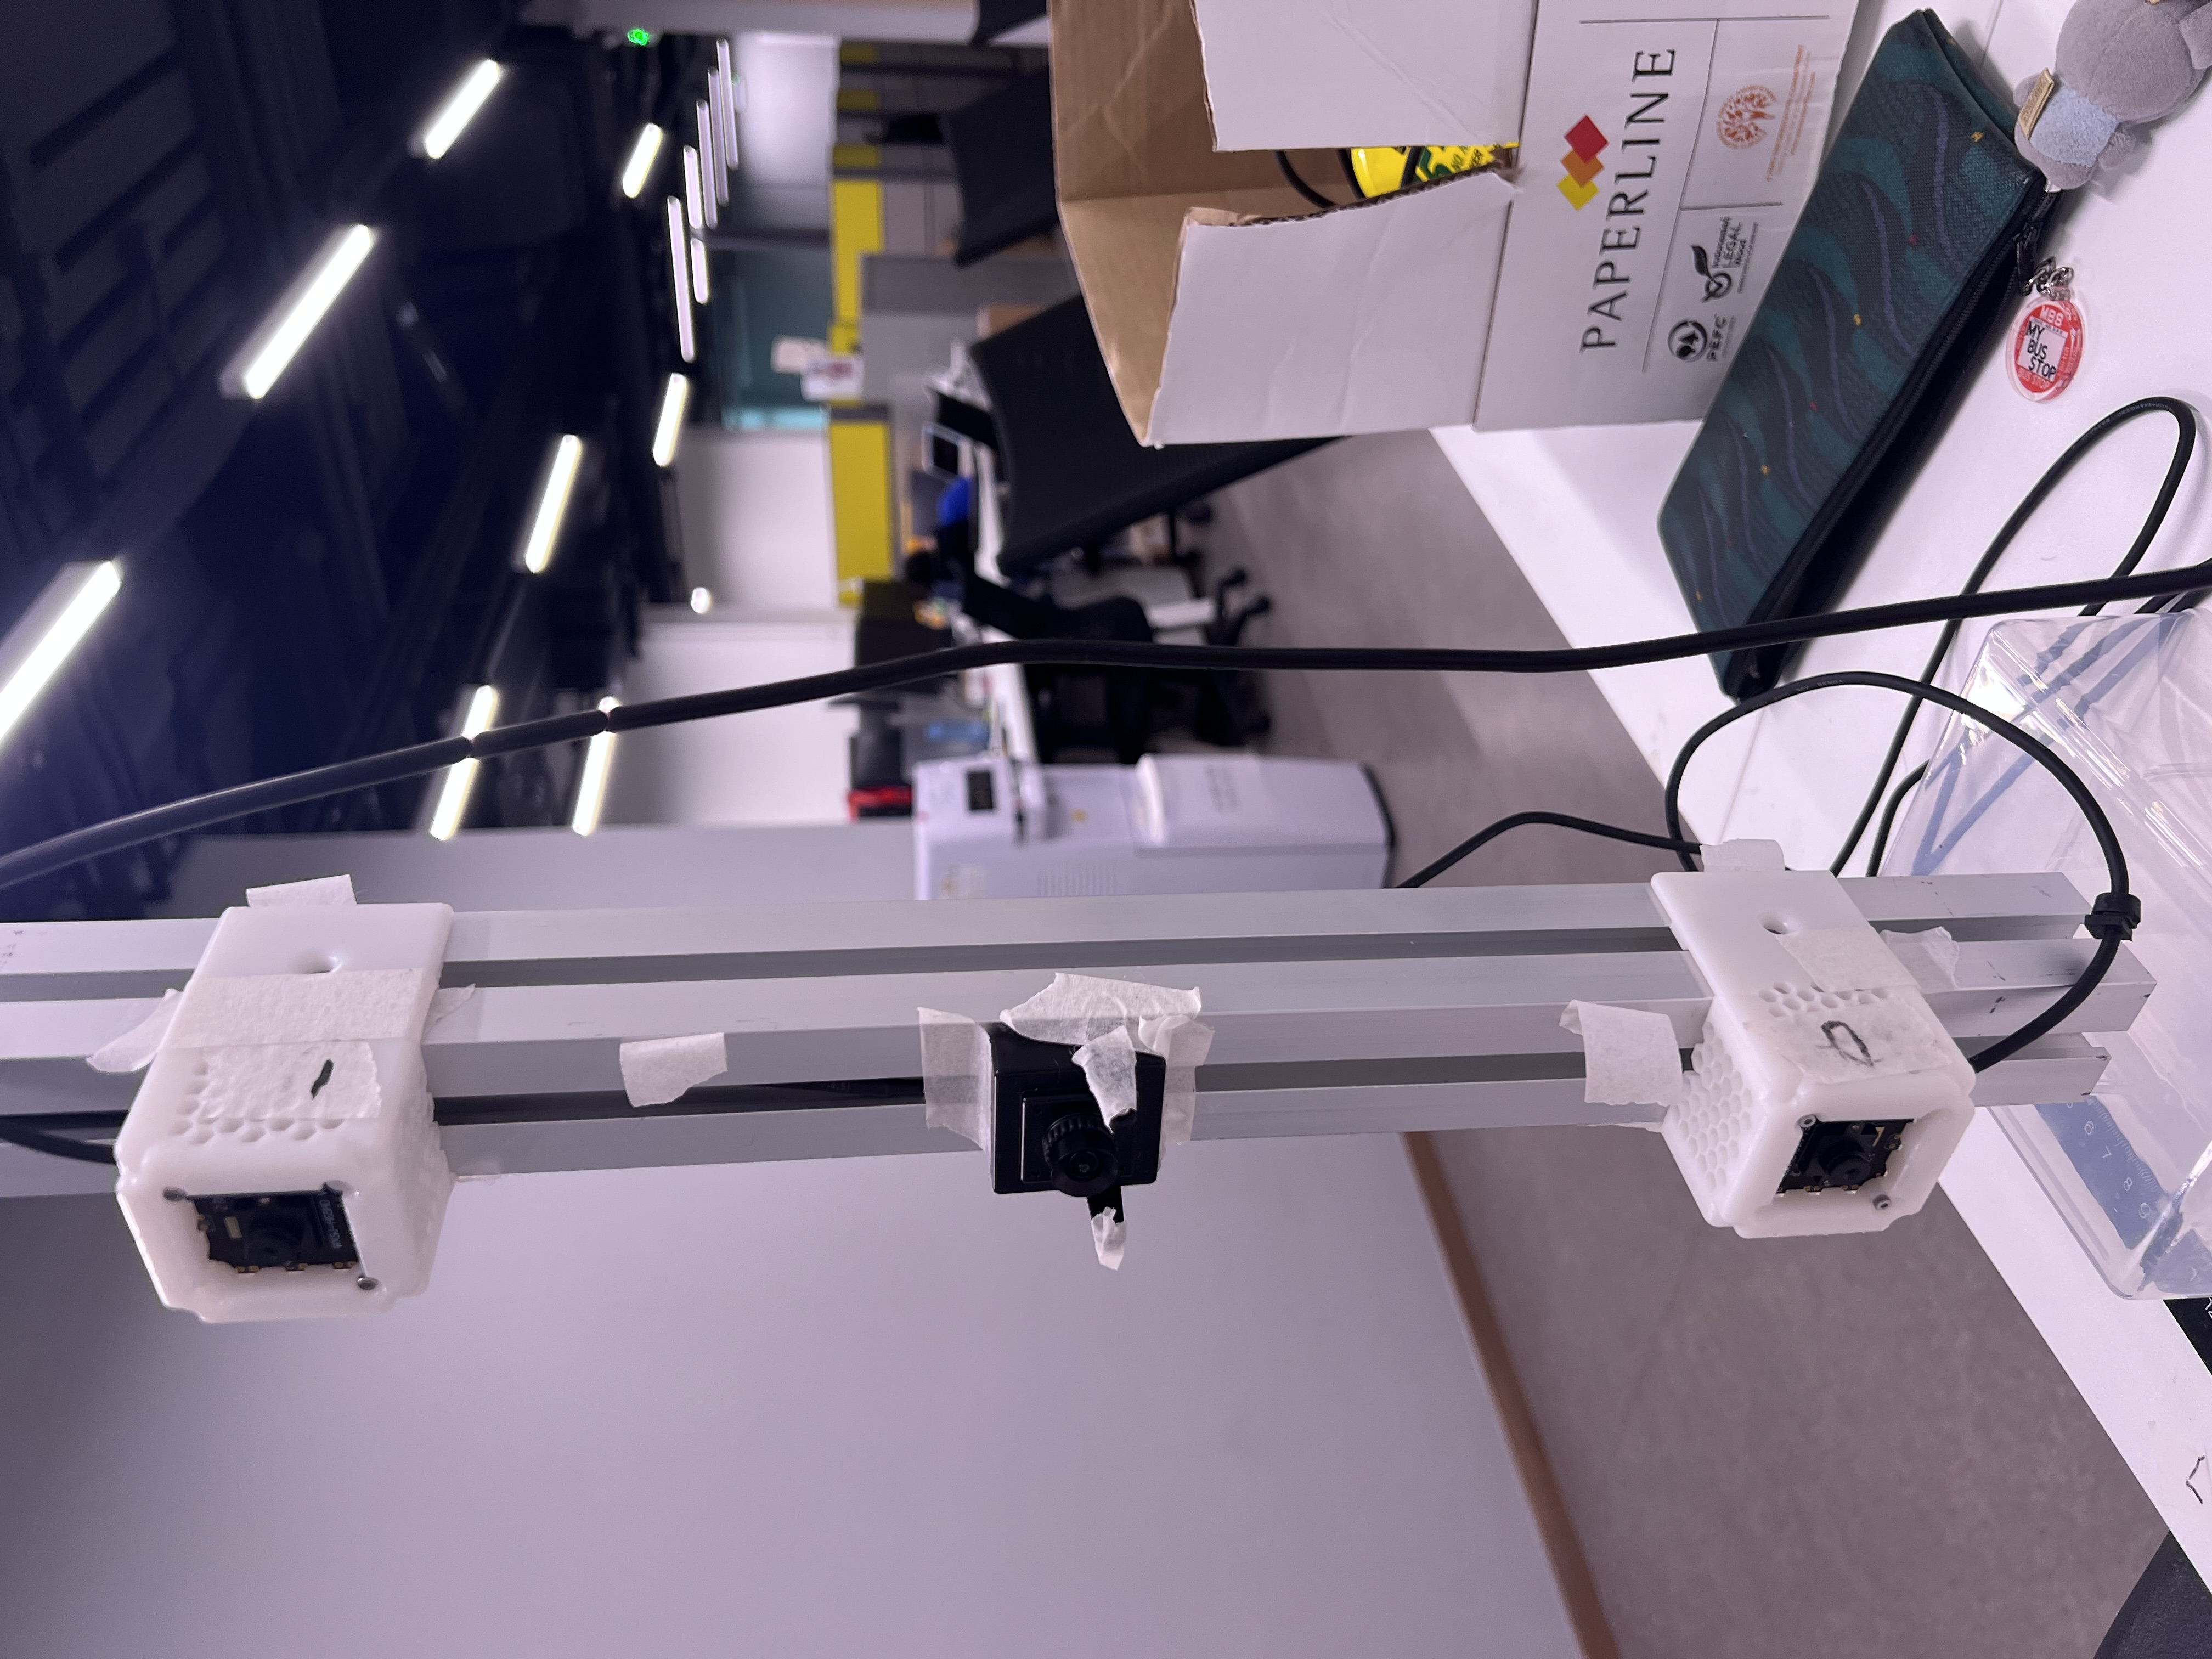
\includegraphics[width=0.6\linewidth]{figures/cameras.jpeg}
                    }
                    \caption{Three-camera setup used for initial chessboard calibration data collection. Cameras are positioned to capture overlapping views of the calibration pattern from multiple angles, ensuring sufficient geometric diversity for robust intrinsic parameter estimation.}
                    \label{collection array}
                \end{figure}
                \begin{figure}
                    \centering
                    \rotatebox{180}{
                    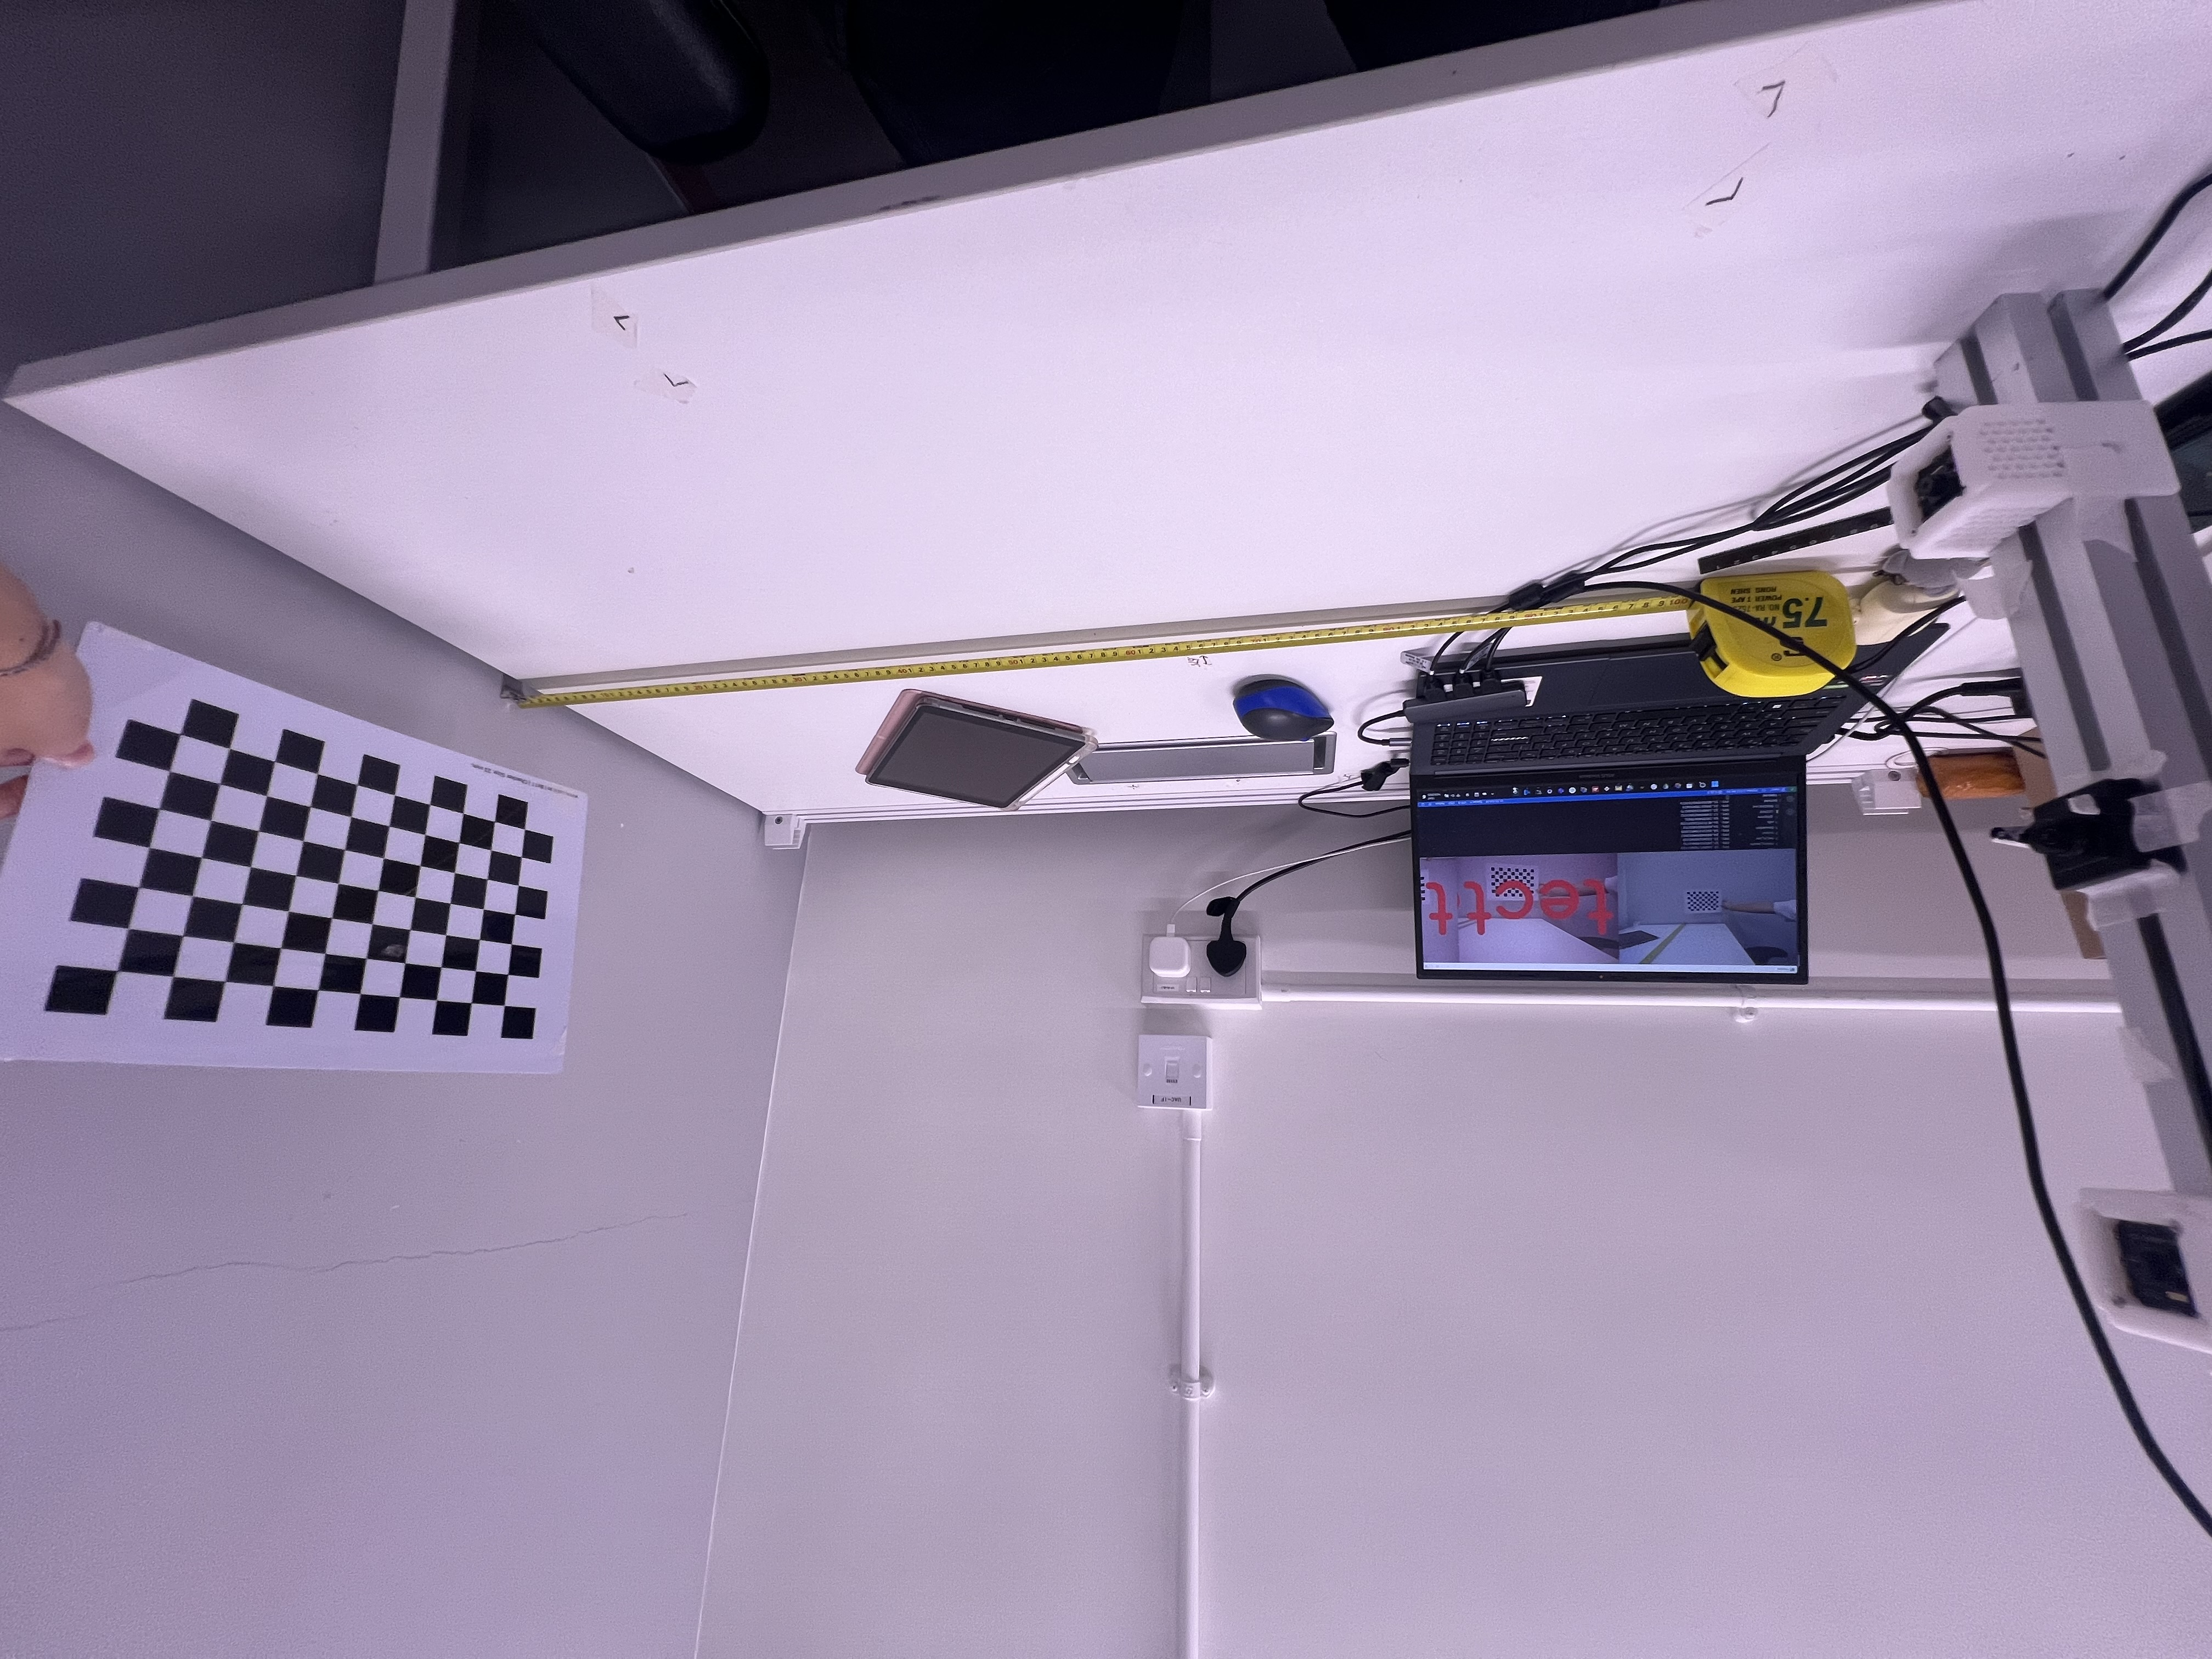
\includegraphics[width=0.6\linewidth]{figures/detected.jpeg}
                    }
                    \caption{Chessboard corner detection validation showing successful identification of 8×11 internal corners. The overlaid grid confirms proper pattern recognition, with corner coordinates used for camera calibration parameter estimation.}
                    \label{validation}
                \end{figure}
                \begin{figure}
                    \centering
                    \rotatebox{0}{
                    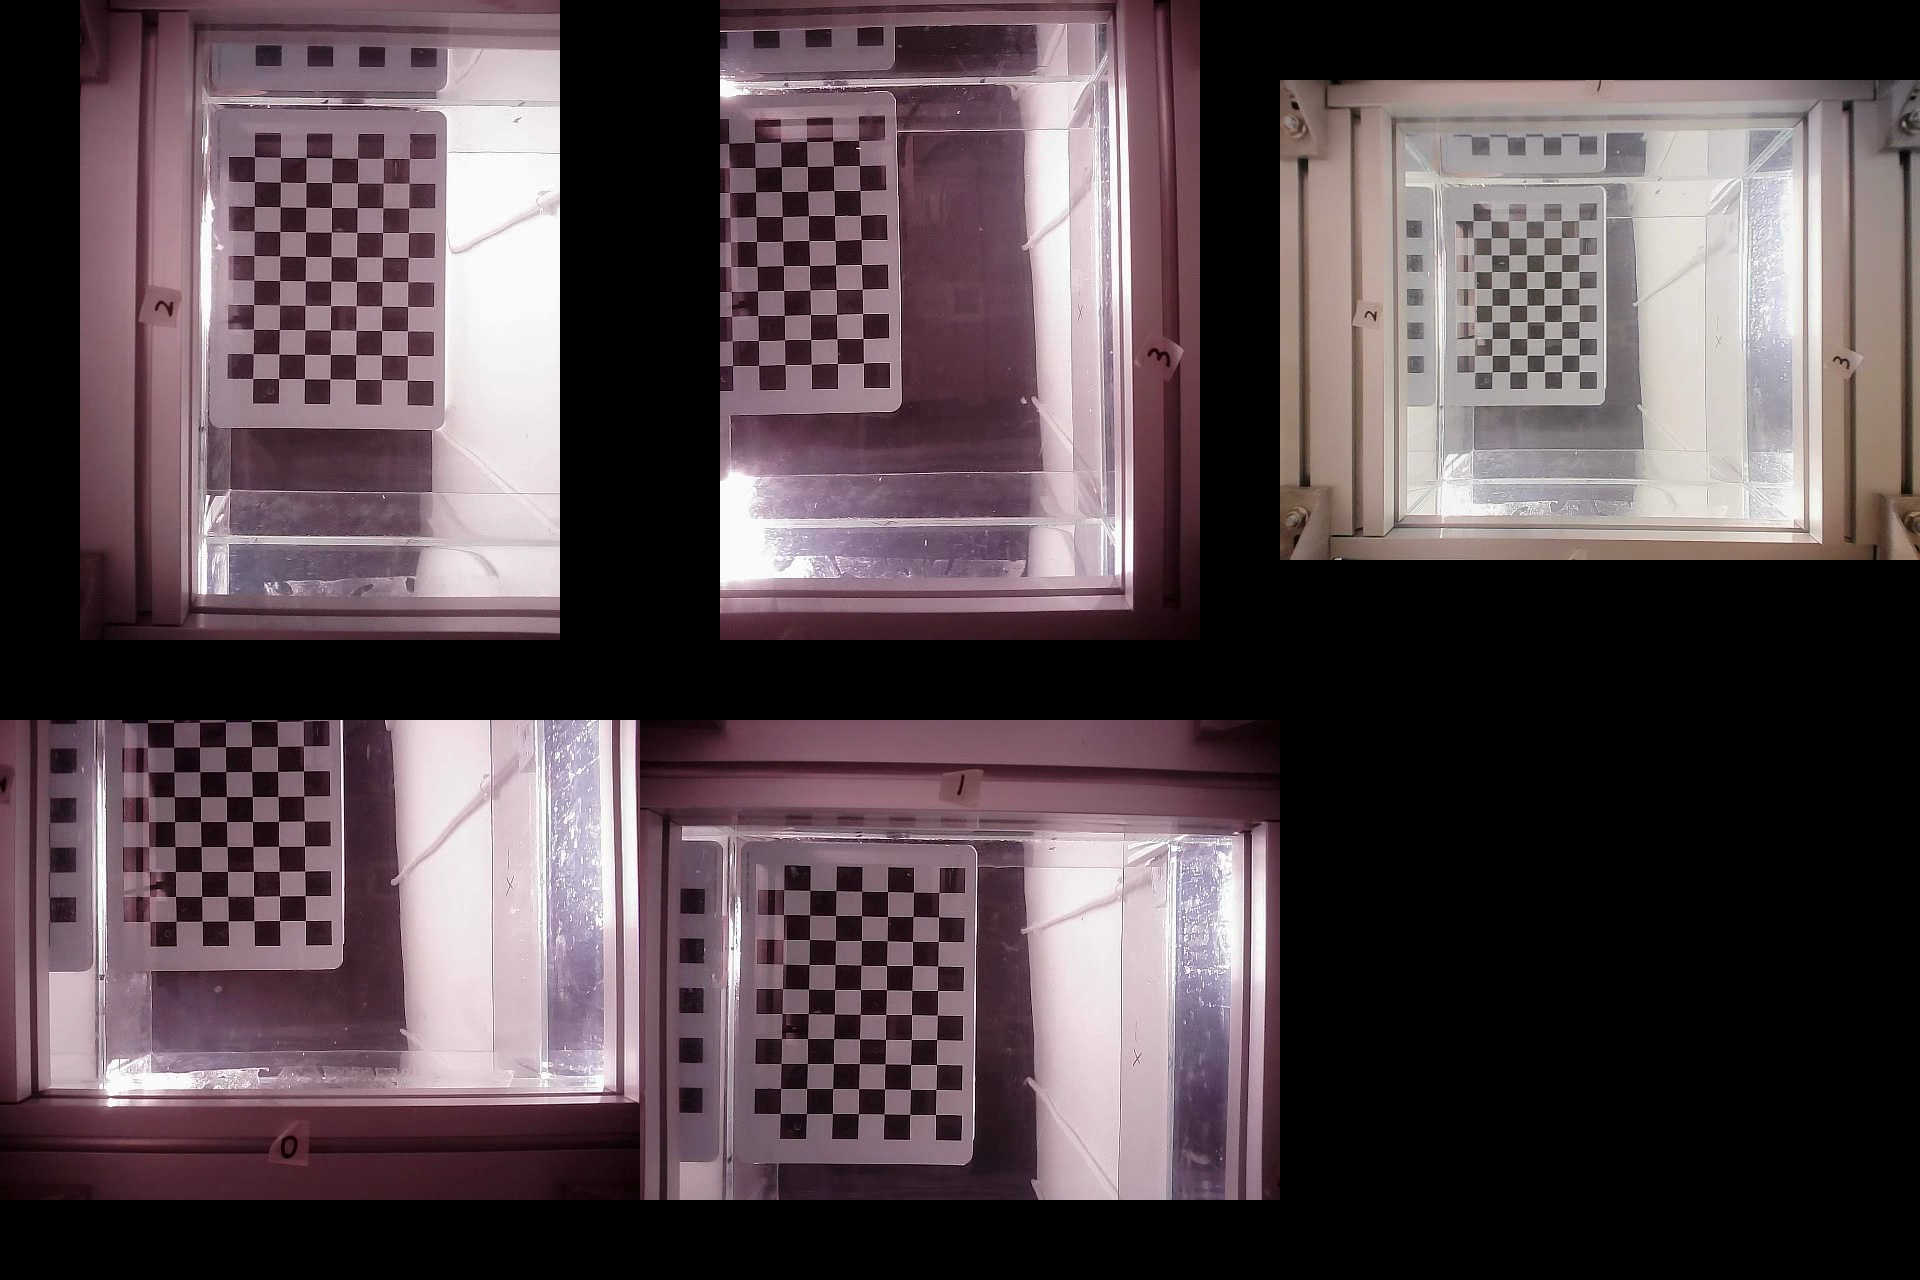
\includegraphics[width=0.6\linewidth]{figures/multi_cameras.jpg}
                    }
                    \caption{Synchronized video frames from five cameras showing simultaneous capture of the chessboard pattern. Time synchronization ensures consistent object points across all camera views, enabling accurate extrinsic parameter calibration between camera coordinate systems.}
                    \label{multi_cameras}
                \end{figure}
                \begin{figure}
                    \centering
                    \rotatebox{0}{
                    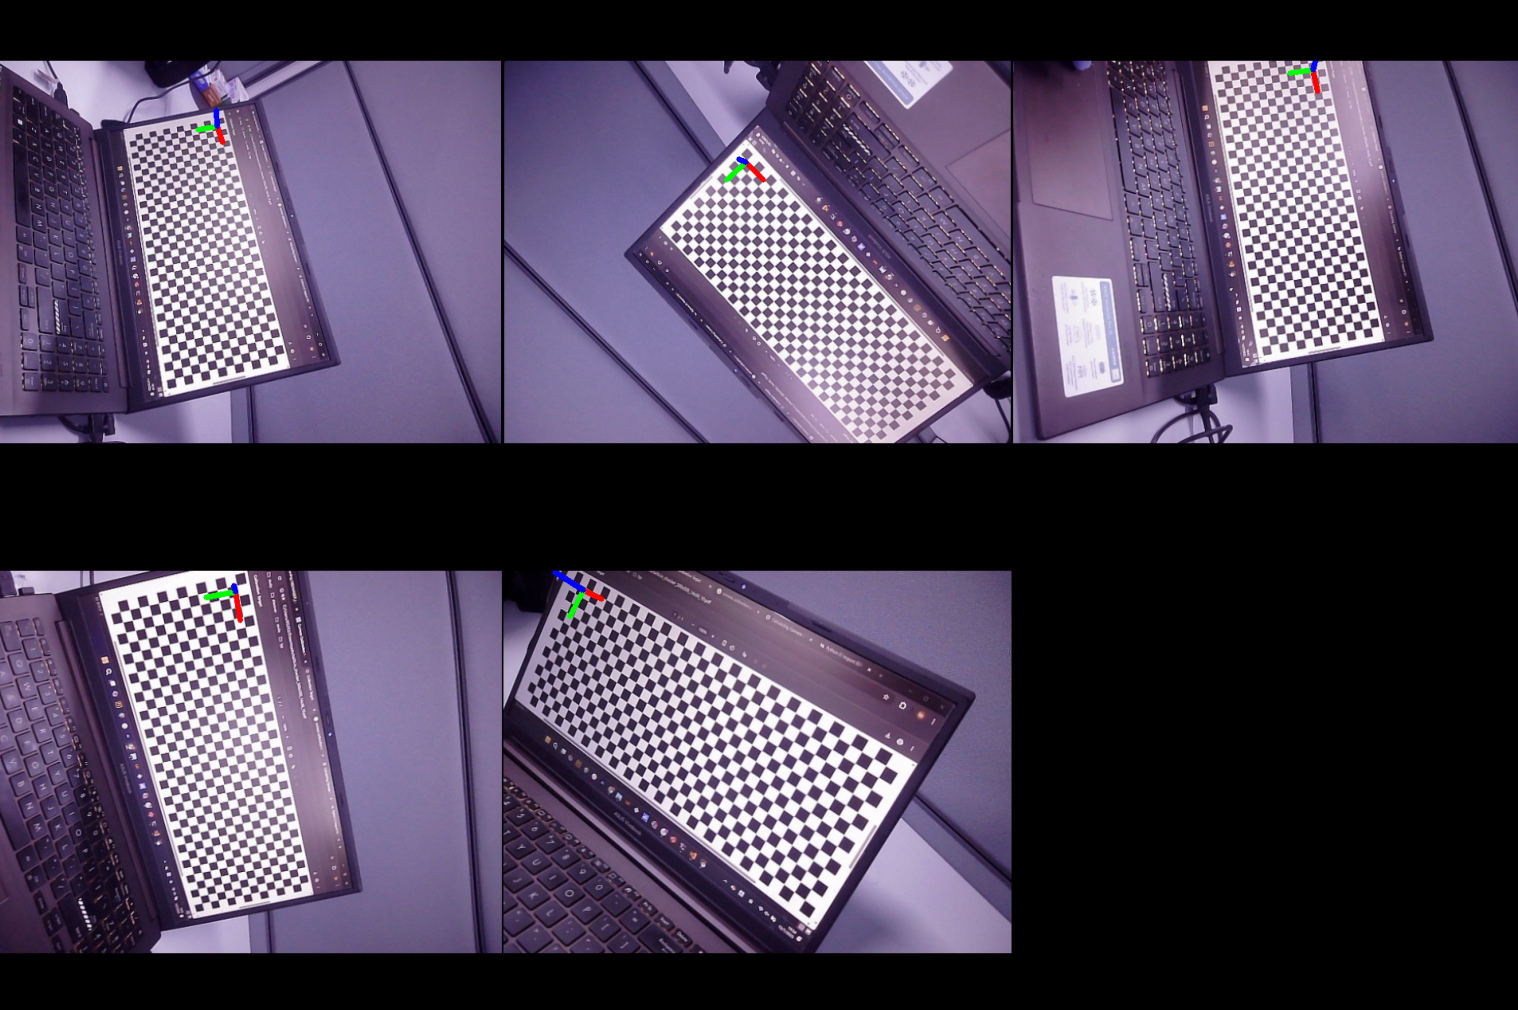
\includegraphics[width=0.6\linewidth]{figures/arrow.png}
                    }
                    \caption{Visualization of detected chessboard corners with overlaid coordinate axes. The red circles mark detected corner positions used for establishing the world coordinate system and computing camera projection matrices.}
                    \label{chessboard}
                \end{figure}

            \item \textbf{Task 2.2: ChArUco photo collection}\\\\
                \textbf{Aim:}  Get ChArUco photos suitable for both intrinsic and extrinsic calibrations of all the cameras and achieve better results under water compared to chess chessboard.\\
                \textbf{Expected Outcome:} Valid photos are collected, so that part of the ChArUco can be captured by all the cameras in the same frame, and at least 6 points of the board can be further extracted and matched with the object points.\\
                \textbf{Group member in charge:} XU, Borong\\
                \textbf{Work:} To overcome the poor performance of the chessboard underwater, we use a different type of calibration board. Similar to Task 2.1, we wrote a Python program to collect frames of a ChArUco board with $8\times11$ 23mm squares covering as many camera angles as possible, while outputting ChArUco detection results for validation, as shown in Figure~\ref{ChArUco}.\\\\
                The ChArUco board is similar to a chessboard but has several ArUco markers embedded inside the pattern. This allows the detection algorithm to extract image points without requiring the entire board to be visible. With this advantage, our experiment demonstrates stable detection underwater, especially for extrinsic calibration.
                \begin{figure}
                    \centering
                    \rotatebox{0}{
                    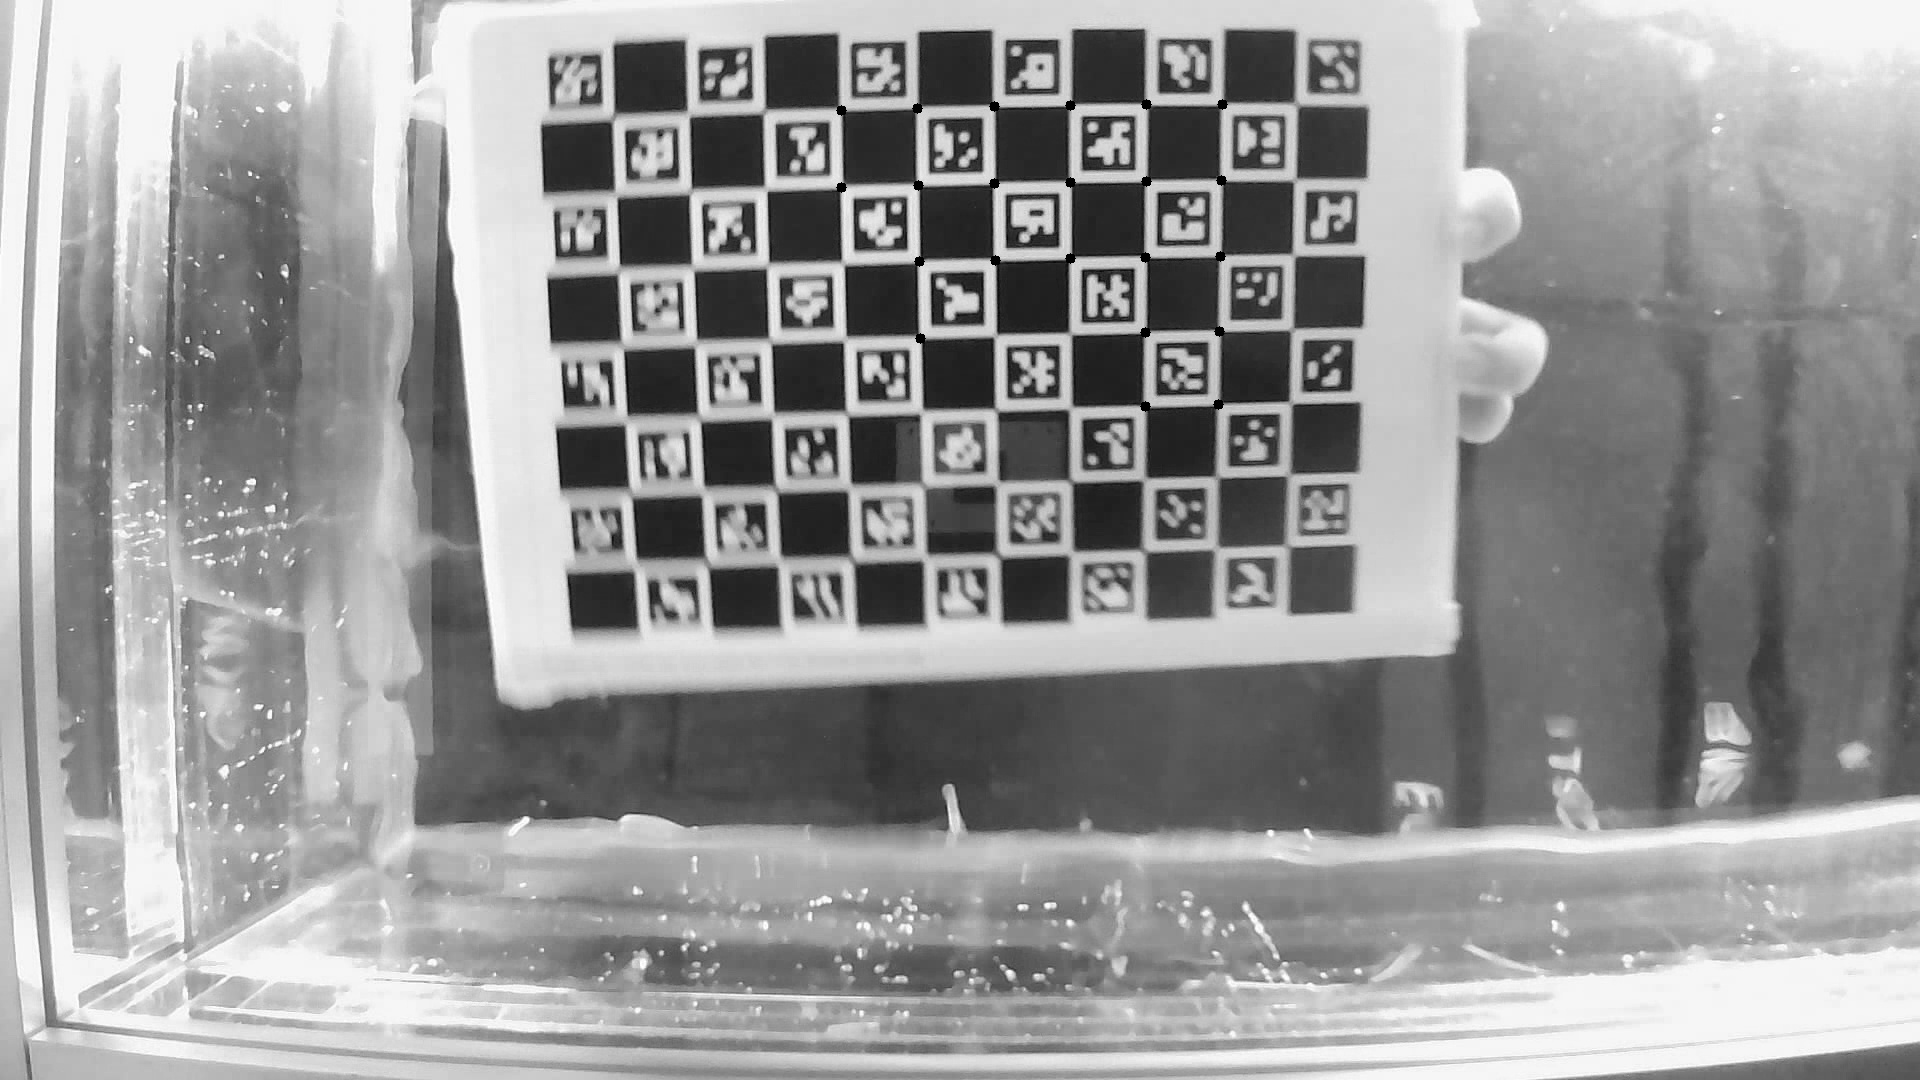
\includegraphics[width=0.6\linewidth]{figures/charuco.jpg}
                    }
                    \caption{ChArUco calibration board with detected corner points marked in green. The embedded ArUco markers enable robust underwater detection even when only partial board segments are visible, overcoming limitations of traditional chessboard patterns in refractive environments.}
                    \label{ChArUco}
                \end{figure}

            
            \item \textbf{Task 2.3: Intrinsic Parameter Calibration}\\\\
            \textbf{Aim:} Calibrate the intrinsic parameters of all the cameras.\\
            \textbf{Expected Outcome:} Error has to be within $7.0\times10^{-2}$m.\\
            \textbf{Group member in charge:} Both members\\
            \textbf{Work:} We wrote an algorithm for the intrinsic calibration of the cameras first. Then we input the collected chessboard photos, and the algorithm outputs focal length ($f_x$, $f_y$), principal point ($c_x$, $c_y$), and distortion coefficients for each of the 5 USB cameras(Equation~\ref{int_param}). \\\\
            \begin{equation}
            P_0
            = \begin{bmatrix}x_0 \\ y_0 \\ z\end{bmatrix}
            =
            \begin{bmatrix}
            f_x & 0 & c_x & 0 \\
            0 & f_y & c_y & 0 \\
            0 & 0 & 1 & 0
            \end{bmatrix}
            \begin{bmatrix}x \\ y \\ z \\ 1\end{bmatrix}
            = MP
            \label{int_param}
            \end{equation}
            where $P_0$ is the projected 2D image point, $M$ is the camera intrinsic matrix with focal lengths $f_x$, $f_y$ and principal point coordinates $c_x$, $c_y$, and $P$ is the 3D world point in homogeneous coordinates.
            After that, reprojection error analysis was used to validate calibration quality. Recently, the error is $7.1\times10^{-2}$m, which is close to but still does not meet our expected outcome.\\\\
            
            At first, we got the value of error significantly different from the requirement. We were using videos with a total length of 3 minutes, and each camera had around 40 valid captures on average at that time. We found that the amount of input might not be enough, so we recorded more videos with a total length of 8 minutes. As a result, around 90 valid captures were received on average from each camera, which reduced the error and got closer to the requirement.\\\\
            The distortion parameter included in the intrinsic parameter can undistort the image for further application(Figure~\ref{undistrot}). The performance of the undistortion algorithm can shape the detection accuracy of our system under complex light environments (e.g., with underwater light refraction).

            \begin{figure}
                    \centering
                    \rotatebox{0}{
                    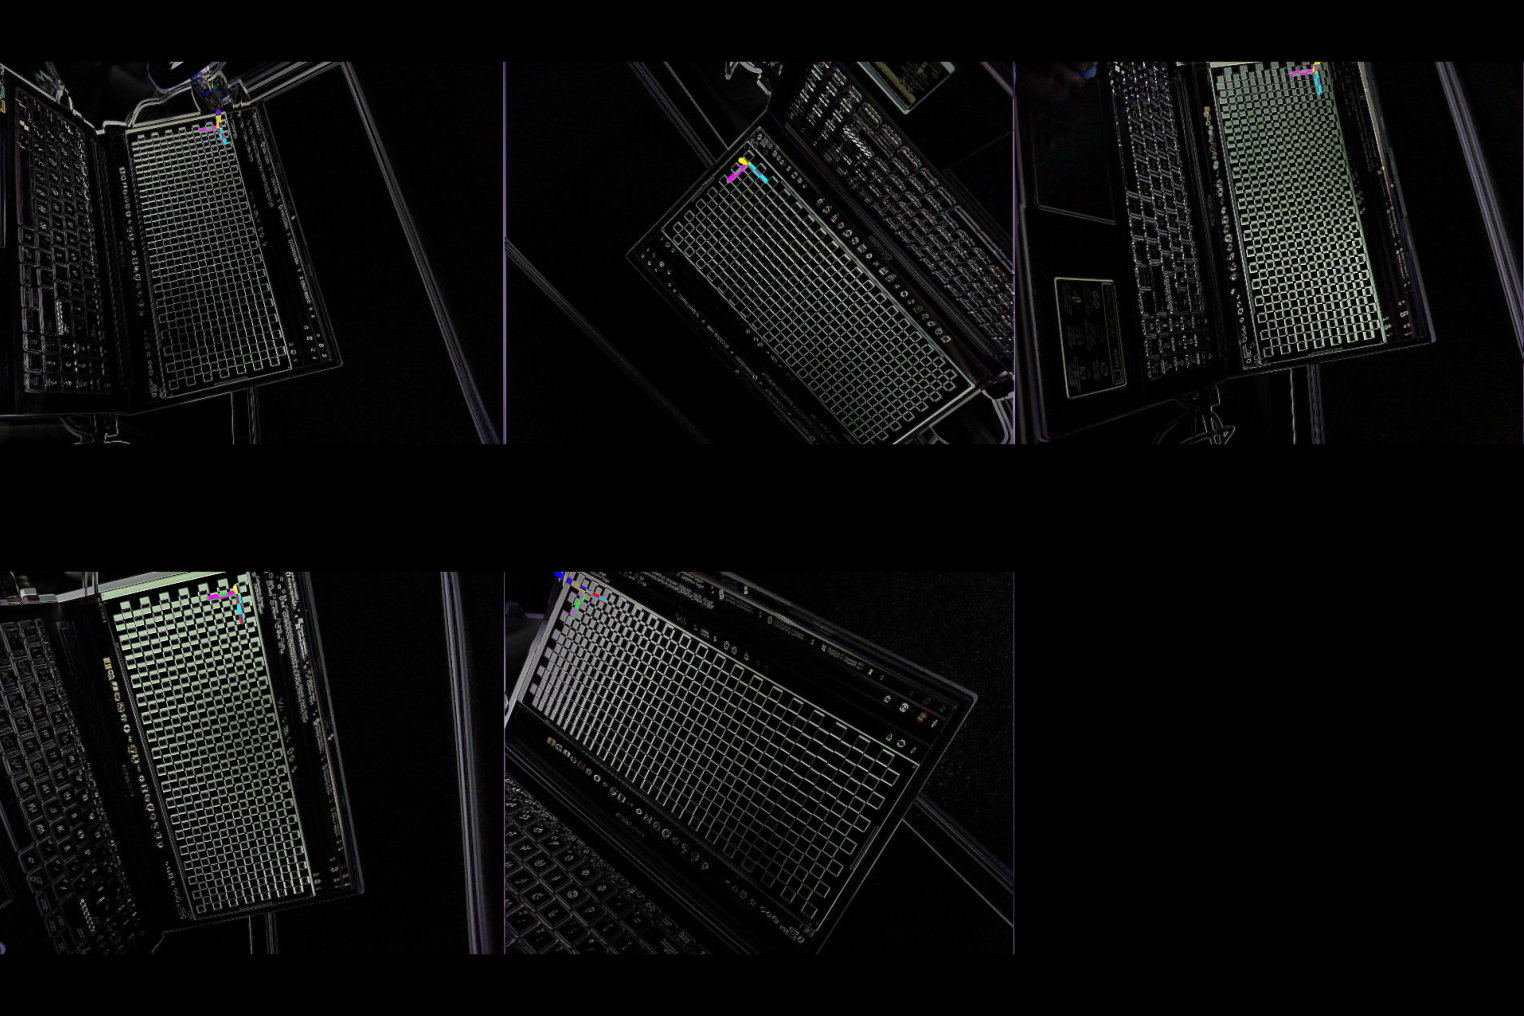
\includegraphics[width=0.6\linewidth]{figures/undistort.png}
                    }
                    \caption{Comparison of distorted (left) and undistorted (right) images showing barrel distortion correction using intrinsic calibration parameters. The radial distortion coefficients compensate for lens imperfections, ensuring accurate marker detection and pose estimation.}
                    \label{undistrot}
            \end{figure}
            
            \item \textbf{Task 2.4: Extrinsic Parameter Calibration}\\\\
            \textbf{Aim:} Calibrate the extrinsic parameters of all the cameras.\\
            \textbf{Expected Outcome:} Error has to be within $2.0\times10^{-2}$m.\\
            \textbf{Group member in charge:} XU, Borong\\\
            \textbf{Work:} We wrote an algorithm using stereo calibration techniques to determine relative camera positions and orientations between the center wide-angle camera and the other side cameras. Then we input the collected chessboard photos, and the algorithm outputs homogeneous transformation matrices between cameras. A world coordinate system was established with the center camera as the reference frame, and reprojection error analysis was also used in this step to validate calibration quality. We also roughly validated the extrinsic calibration results by visualizing the relative positions between the cameras (Figure~\ref{ext_result}), which matches our physical measurements of the camera array.\\\\
            \begin{equation}
            \begin{aligned}
                T &= \argmin_T||P_B - (P_A + T)||^2\\
                R & = \argmin_R||P_B - (RP_A + T)||^2\\
            \end{aligned}
            \label{ext_goal}
            \end{equation}
            \begin{figure}
                    \centering
                    \rotatebox{0}{
                    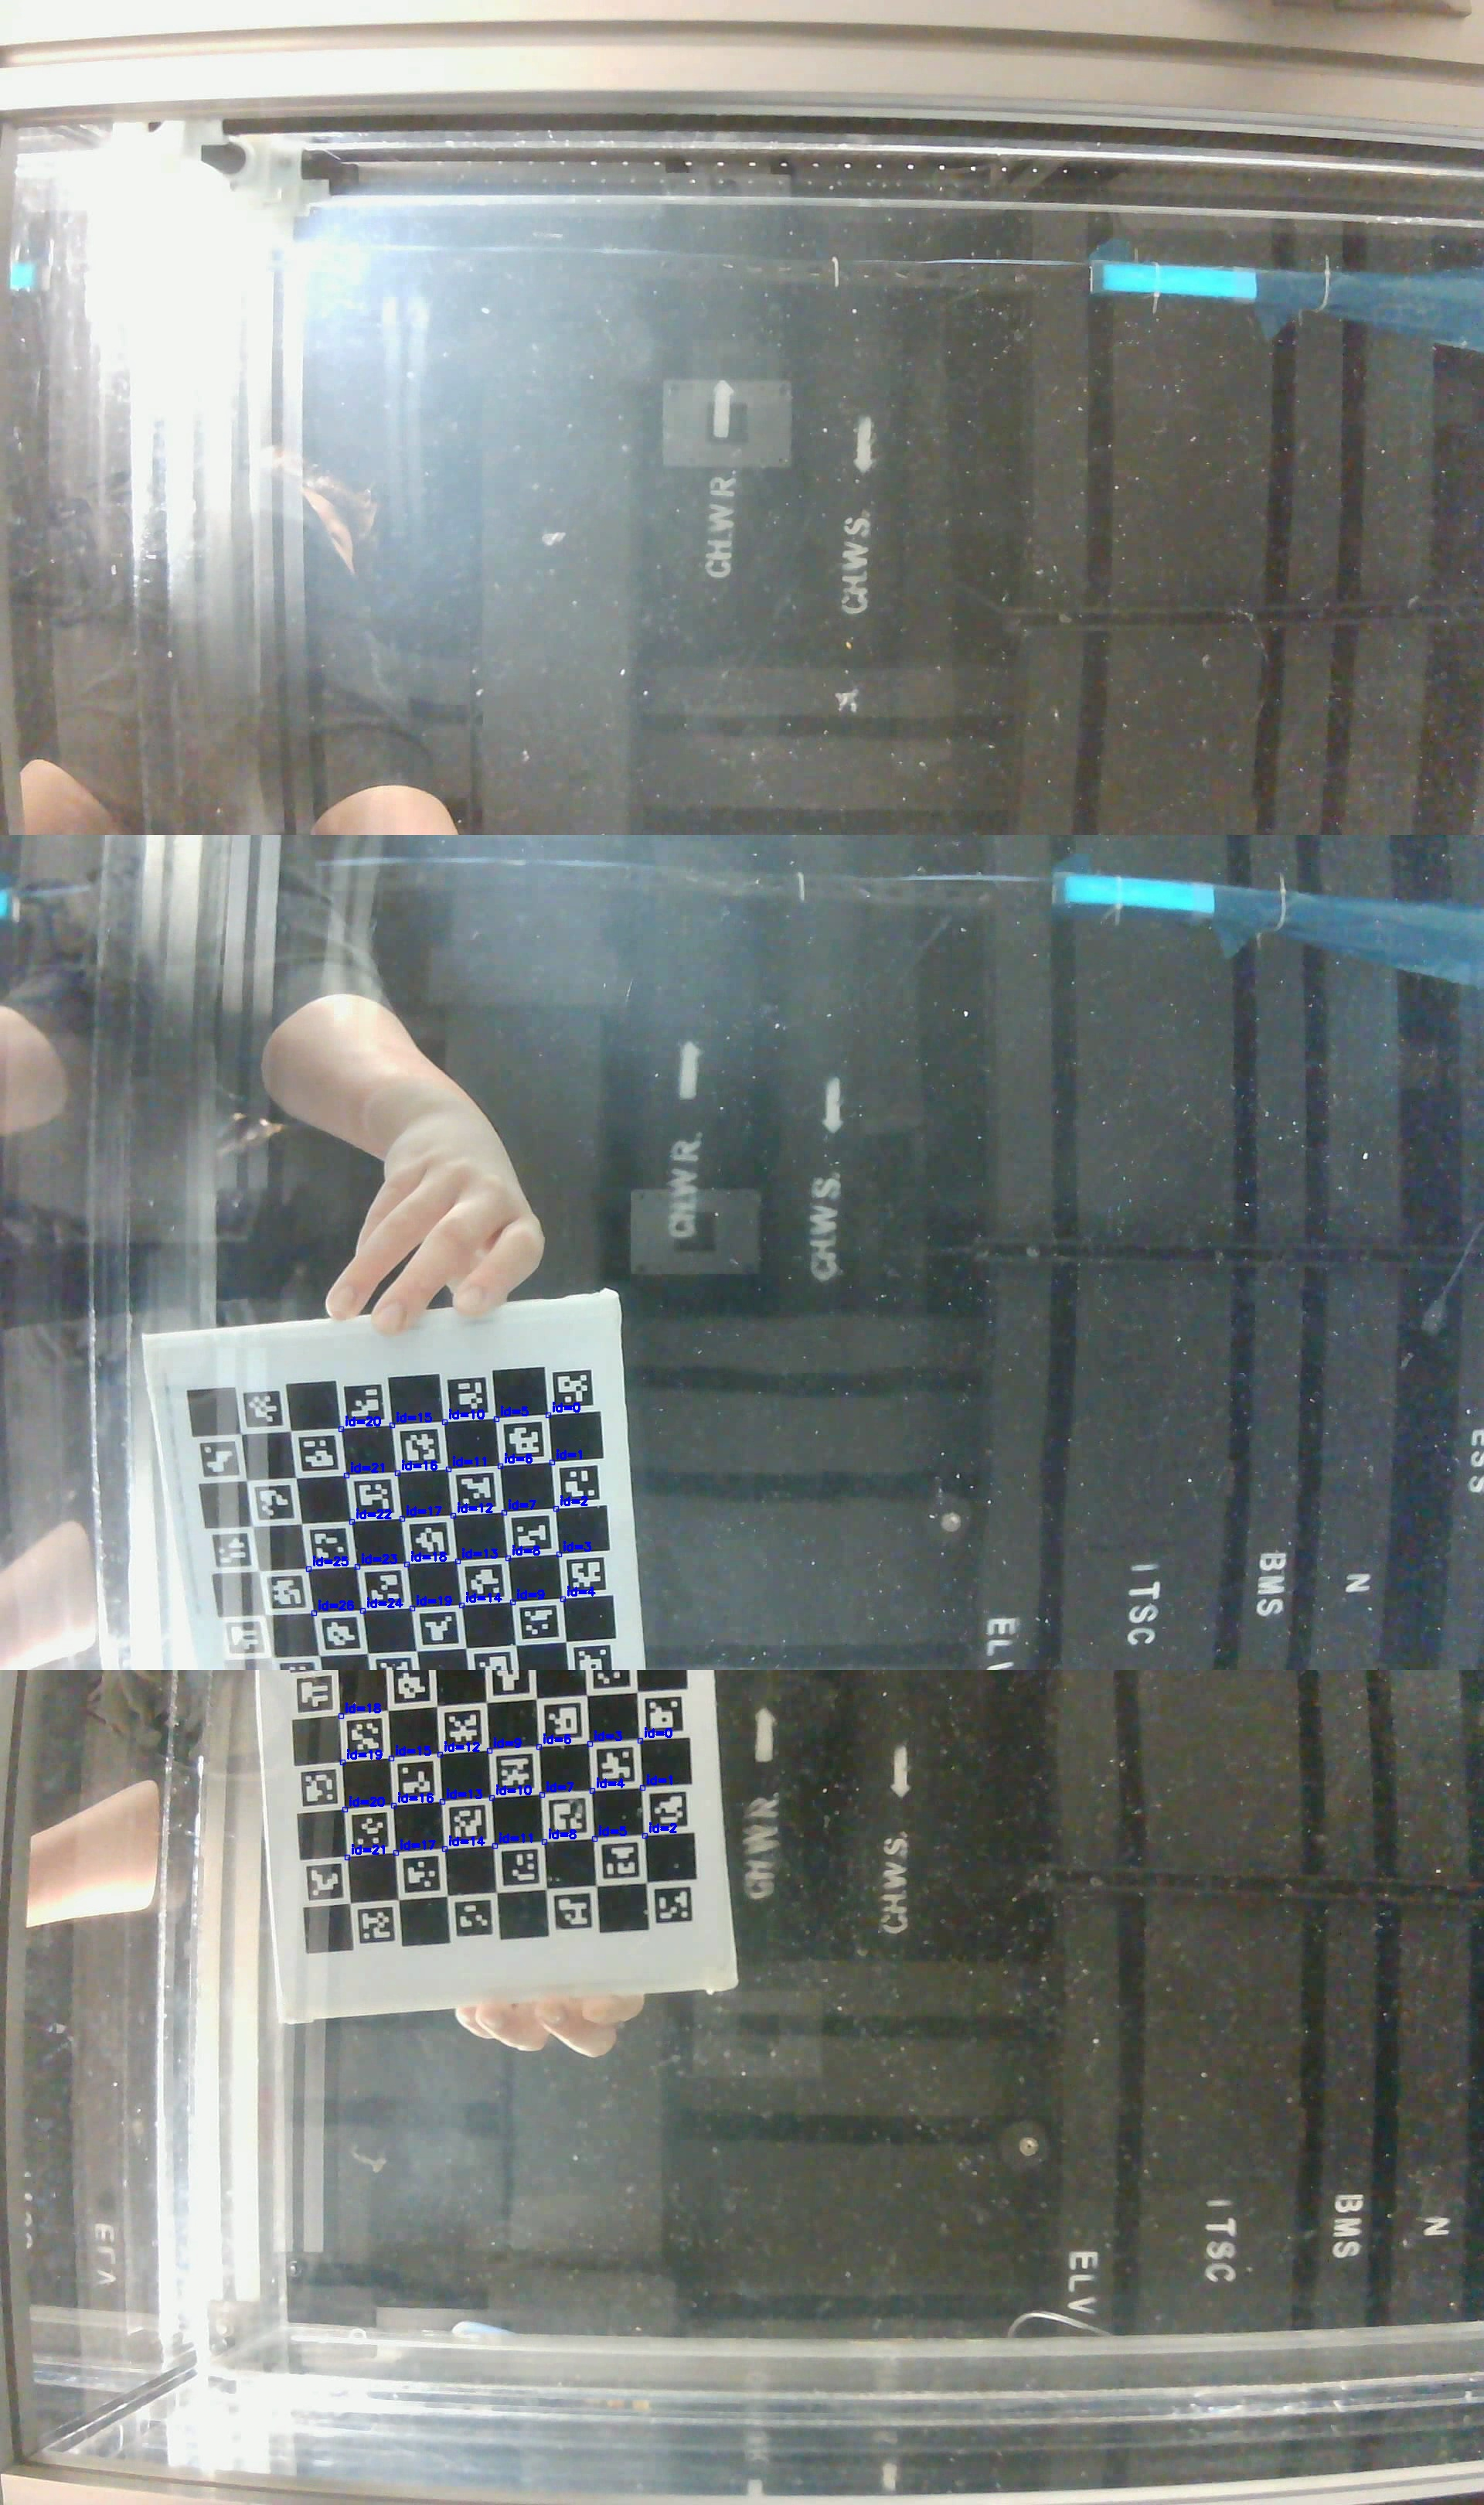
\includegraphics[width=0.6\linewidth]{figures/charuco_capture.jpg}
                    }
                    \caption{Capture of a ChArUco board in the cross section between two cameras.}
                    \label{charuco_capture}
            \end{figure}
            In the underwater setting, the field of view of each camera is insufficient to capture the entire chessboard in two camera frames simultaneously, making the traditional extrinsic calibration method inadequate. We propose a new method using the ChArUco board to calibrate the camera extrinsic parameters (Figure~\ref{charuco_capture}). This method utilizes PnP solvers to find each camera's relative transformation to the ChArUco calibration board, producing pairs of camera locations. With the camera point correspondences, we can solve the transformation between cameras (Equation~\ref{ext_goal}), where $T$ is the optimal translation vector and $R$ is the optimal rotation matrix that minimize the Euclidean distance between corresponding 3D points $P_A$ and $P_B$ in different camera coordinate systems.

            Similar to intrinsic calibration, initial extrinsic calibration results showed higher errors due to insufficient calibration data. Increasing the number of valid captures reduced the transformation error and improved calibration accuracy.

            \begin{figure}
                    \centering
                    \rotatebox{0}{
                    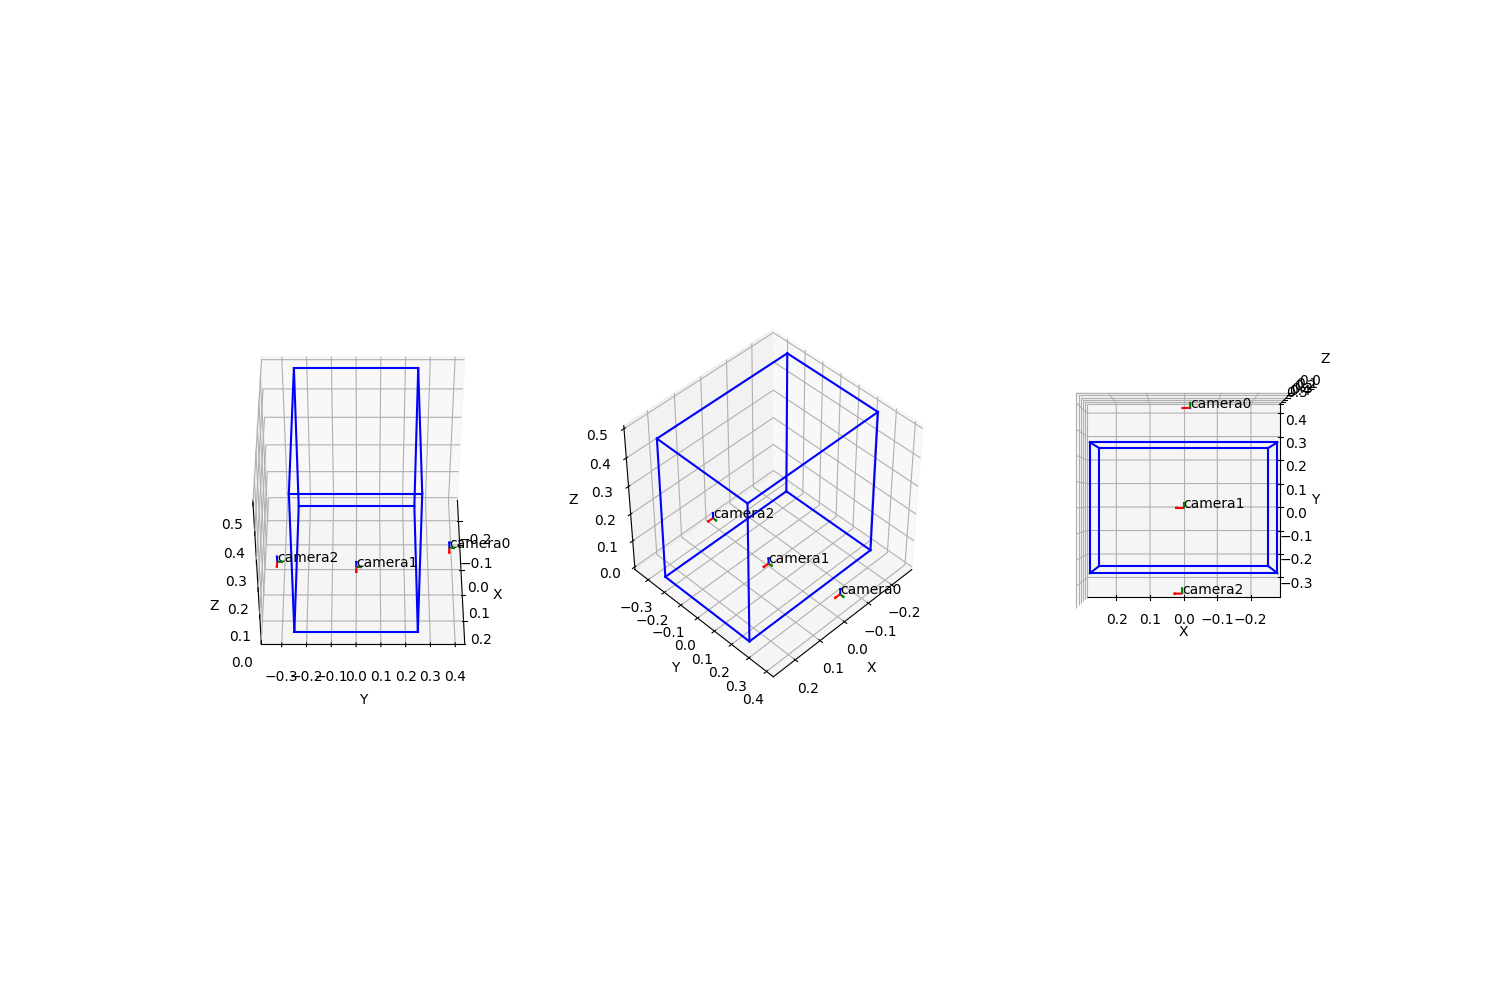
\includegraphics[width=0.6\linewidth]{figures/visualize_ext.png}
                    }
                    \caption{3D visualization of calibrated camera positions and orientations showing the extrinsic calibration results. The coordinate frames represent each camera's pose relative to the world coordinate system, with transformation matrices enabling consistent multi-camera localization.}
                    \label{ext_result}
            \end{figure}
            
            \item \textbf{Task 2.5: Underwater Calibration Adjustment}\\\\
            \textbf{Aim:} Find the differences in calibration parameters in air and water.\\
            \textbf{Expected Outcome:} Get the correction factor of calibration parameters from air to water.\\
            \textbf{Group member in charge:} XU, Borong\\\
            \textbf{Work:} We repeated intrinsic calibration underwater and discovered that the calibration results failed in underwater environments. This could be due to light refraction when crossing different media. \\
            To test the effectiveness of the intrinsic calibration results, we use the extrinsic calibration results to compare the localization between different cameras. Since the extrinsic parameters consist of transformations between cameras, they are not affected by light refraction. Once the extrinsic parameters are confirmed effective in air, we can use them to validate the intrinsic parameters produced by our method.\\
            The cross-medium light refraction invalidates the pinhole camera assumption, and the traditional polynomial distortion model is insufficient to estimate the distortion. Therefore, we propose a new method for underwater distortion calibration.\\\\
            Our new method calibrates the camera parameter $K$ and distortion model $D$ separately. We model the distortion parameter $D$ as a vector field. We first apply the OpenCV calibration program with the assumption of no distortion to obtain the intrinsic parameter $K$, and using this $K$ matrix, we normalize the object points and use the undistorted reprojected image points as ground truth for the distortion parameters. Then, we calibrate the distortion parameters using gradient descent with PyTorch. Using the new distortion model, we undistort the image points and recalibrate the intrinsic parameter $K$.\\\
            \begin{algorithm}
            \caption{Separate K and Distortion Calibration}\label{alg:distortion_calibration}
            \begin{algorithmic}
            \Require Object points $\{\mathbf{Q}_i\}$, observed image points $\{\mathbf{p}_i\}$, image size
            \Ensure Camera matrix $K$, distortion model $D$
            
            \State \textbf{Step 1: Initial K calibration}
            \State $K, \{R_j, \mathbf{t}_j\} \gets \texttt{calibrateCamera}(\{\mathbf{Q}_i\}, \{\mathbf{p}_i\}, \text{dist}=\mathbf{0})$
            
            \State \textbf{Step 2: Compute reprojected ground truth}
            \For{each view $j$}
                \State $\hat{\mathbf{p}}_j \gets K [R_j \mid \mathbf{t}_j] \, \mathbf{Q}_j$ \Comment{Undistorted ground truth}
            \EndFor
            
            \State \textbf{Step 3: Train distortion model}
            \State Normalize: $\mathbf{x}_d \gets K^{-1} \mathbf{p}$, \quad $\mathbf{x}_t \gets K^{-1} \hat{\mathbf{p}}$
            \State Split $\{(\mathbf{x}_d, \mathbf{x}_t)\}$ into $\mathcal{T}_{\text{train}}$ (80\%) and $\mathcal{T}_{\text{val}}$ (20\%)
            \State Initialize distortion model $D_\theta$
            \For{epoch $= 1$ \textbf{to} $N_{\text{epochs}}$}
                \State $\mathcal{L}_{\text{train}} \gets \frac{1}{|\mathcal{T}_{\text{train}}|} \sum_{(\mathbf{x}_d, \mathbf{x}_t) \in \mathcal{T}_{\text{train}}} \| D_\theta(\mathbf{x}_d) - \mathbf{x}_t \|^2$
                \State $\theta \gets \theta - \eta \nabla_\theta \mathcal{L}_{\text{train}}$
                \State $\mathcal{L}_{\text{val}} \gets \frac{1}{|\mathcal{T}_{\text{val}}|} \sum_{(\mathbf{x}_d, \mathbf{x}_t) \in \mathcal{T}_{\text{val}}} \| D_\theta(\mathbf{x}_d) - \mathbf{x}_t \|^2$
                \If{$\mathcal{L}_{\text{val}} < \mathcal{L}_{\text{val}}^*$}
                    \State $\theta^* \gets \theta$ \Comment{Keep best model}
                \EndIf
            \EndFor
            \State $D \gets D_{\theta^*}$
            
            \end{algorithmic}
            \end{algorithm}

            To reduce the effect of overfitting on the model training, we apply a train validation split of 8:2, and use the model with best performance on the validation set as our final model of distortion.
            For the model of the vector field, we apply a traditional polynomial distortion with radial and tangential components (Equation~\ref{polynomial}), as well as a Multi-Layer Perceptron (MLP) model with tanh activation function to model the nonlinear relationship. The results can be found in Figure~\ref{int_results}.  
            
            \begin{equation}
            \begin{aligned}
            r^2 &= x^2 + y^2 \\
            x' &= x\underbrace{(1 + k_1 r^2 + k_2 r^4 + k_3 r^6)}_{\text{radial}} + \underbrace{2p_1 xy + p_2(r^2 + 2x^2)}_{\text{tangential}} \\
            y' &= y\underbrace{(1 + k_1 r^2 + k_2 r^4 + k_3 r^6)}_{\text{radial}} + \underbrace{p_1(r^2 + 2y^2) + 2p_2 xy}_{\text{tangential}}
            \end{aligned}
            \label{polynomial}
            \end{equation}
            
            \begin{figure}
                    \centering
                    \rotatebox{0}{
                    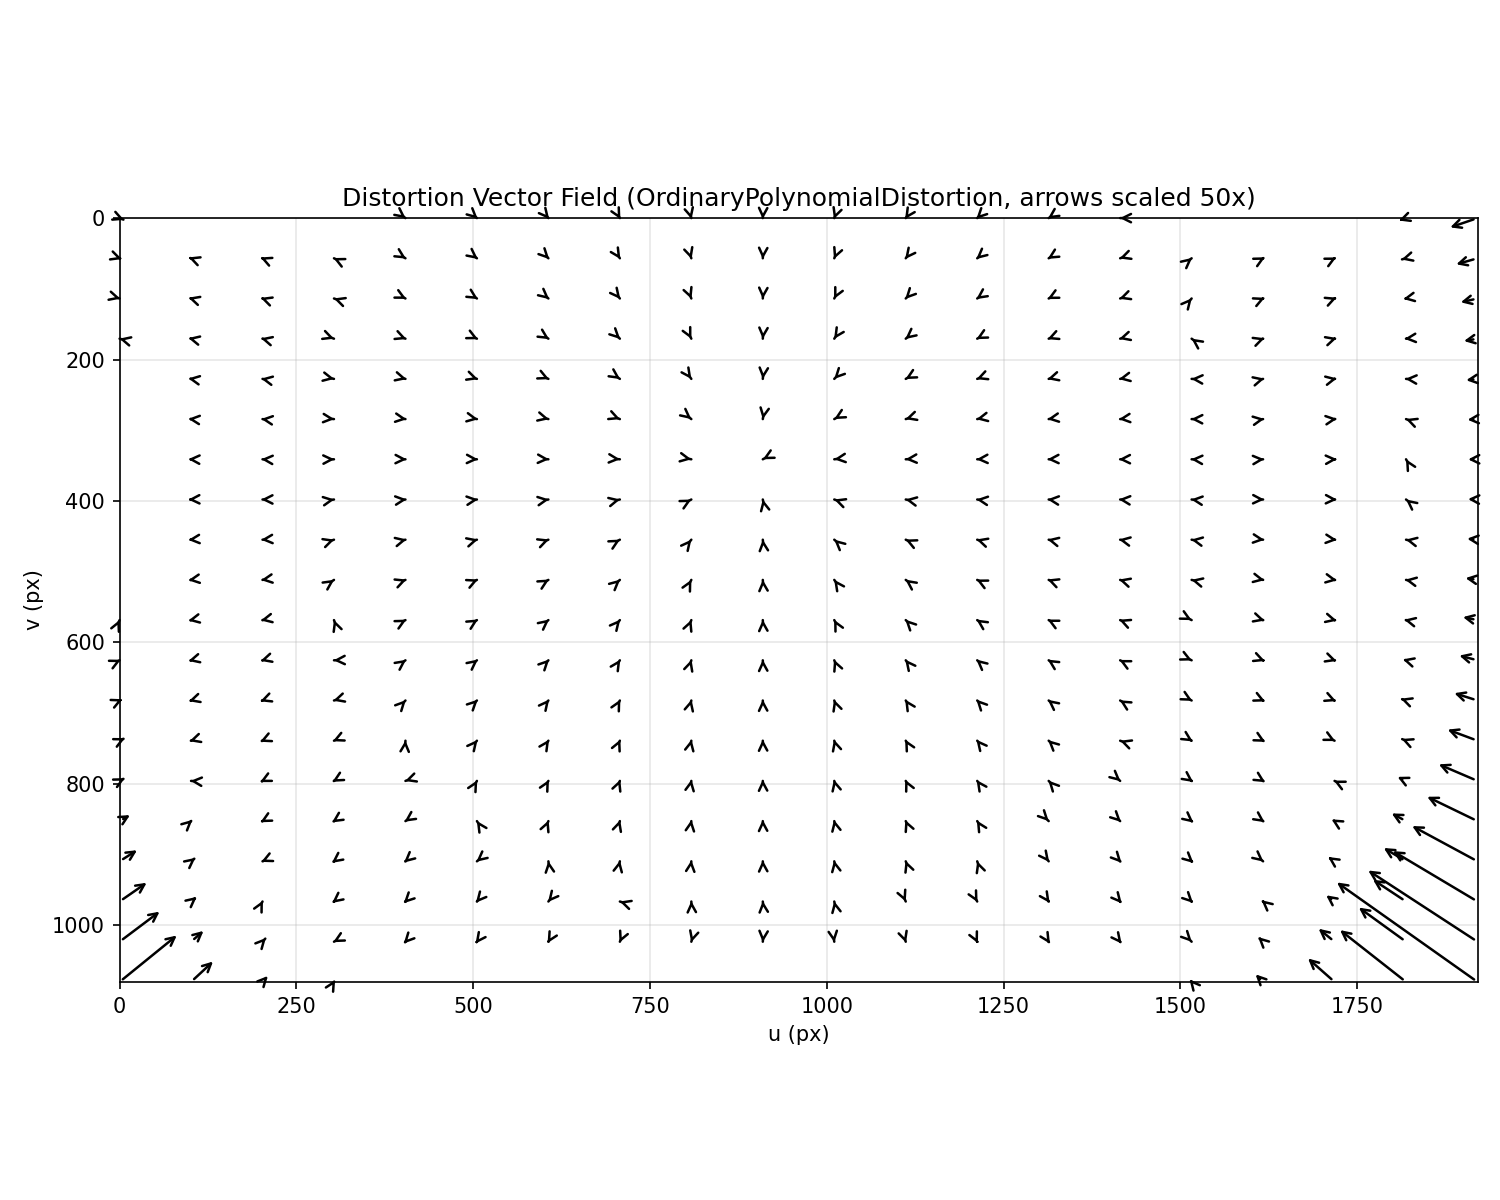
\includegraphics[width=0.6\linewidth]{figures/distortion_field.png}
                    }
                    \caption{Vector field of the camera distortion.}
                    \label{distortion_field}
            \end{figure}
            
            \begin{figure}
                    \centering
                    \rotatebox{0}{
                    
\includegraphics[width=0.6\linewidth]{figures/Placeholder.png}
                    }
                    \caption{Comparison of different method of intrinsic calibration with localization error between cameras with groundtruth extrinsic parameter.}
                    \label{int_results}
            \end{figure}

        \end{itemize}
        
        \subsubsection{Objective Statement 3: ArUco Tracking Implementation}
        The objective is to develop a tracking program based on ArUco marks for AUVs, controlling positional accuracy within $\pm 7\times 10^{-2}$ m and achieving a detection speed of at least 10Hz.
        
        \textbf{Tasks:}
        \begin{itemize}
            \item \textbf{Task 3.1: ArUco Localization Algorithm}\\\\
            \textbf{Aim:} Track ArUco markers of the AUVs.\\
            \textbf{Expected Outcome:} All the AUVs in the water tank can be tracked.\\
            \textbf{Group member in charge:} Both members\\
            \textbf{Work:} We wrote a Python program to implement real-time ArUco marker detection using OpenCV's ArUco module with the DICT\_5X5\_50 dictionary. Robust localization was achieved under varying lighting conditions. When capturing chessboard photos, we also recorded frames of an ArUco marker appearing at five fixed points and moving horizontally along a track (Figure~\ref{aruco test}) to test the algorithm. The algorithm visualized the coordinate axes of the marker and output the frame points associated with it.\\\\
            Before recording those frames, we planned the range of marker locations to be 2~m with 0.5~m between each fixed point. However, the table in the laboratory was not large enough for cameras to capture the marker across such a range. Therefore, the range was narrowed to 0.5~m with 0.125~m between each fixed point. We did not have any rails to move the marker in a straight line, but we found two straight grooves next to the table. We placed the tablet displaying the marker into the groove, which saved time and unnecessary expense.
            \begin{figure}
                \centering
                \rotatebox{-90}{
                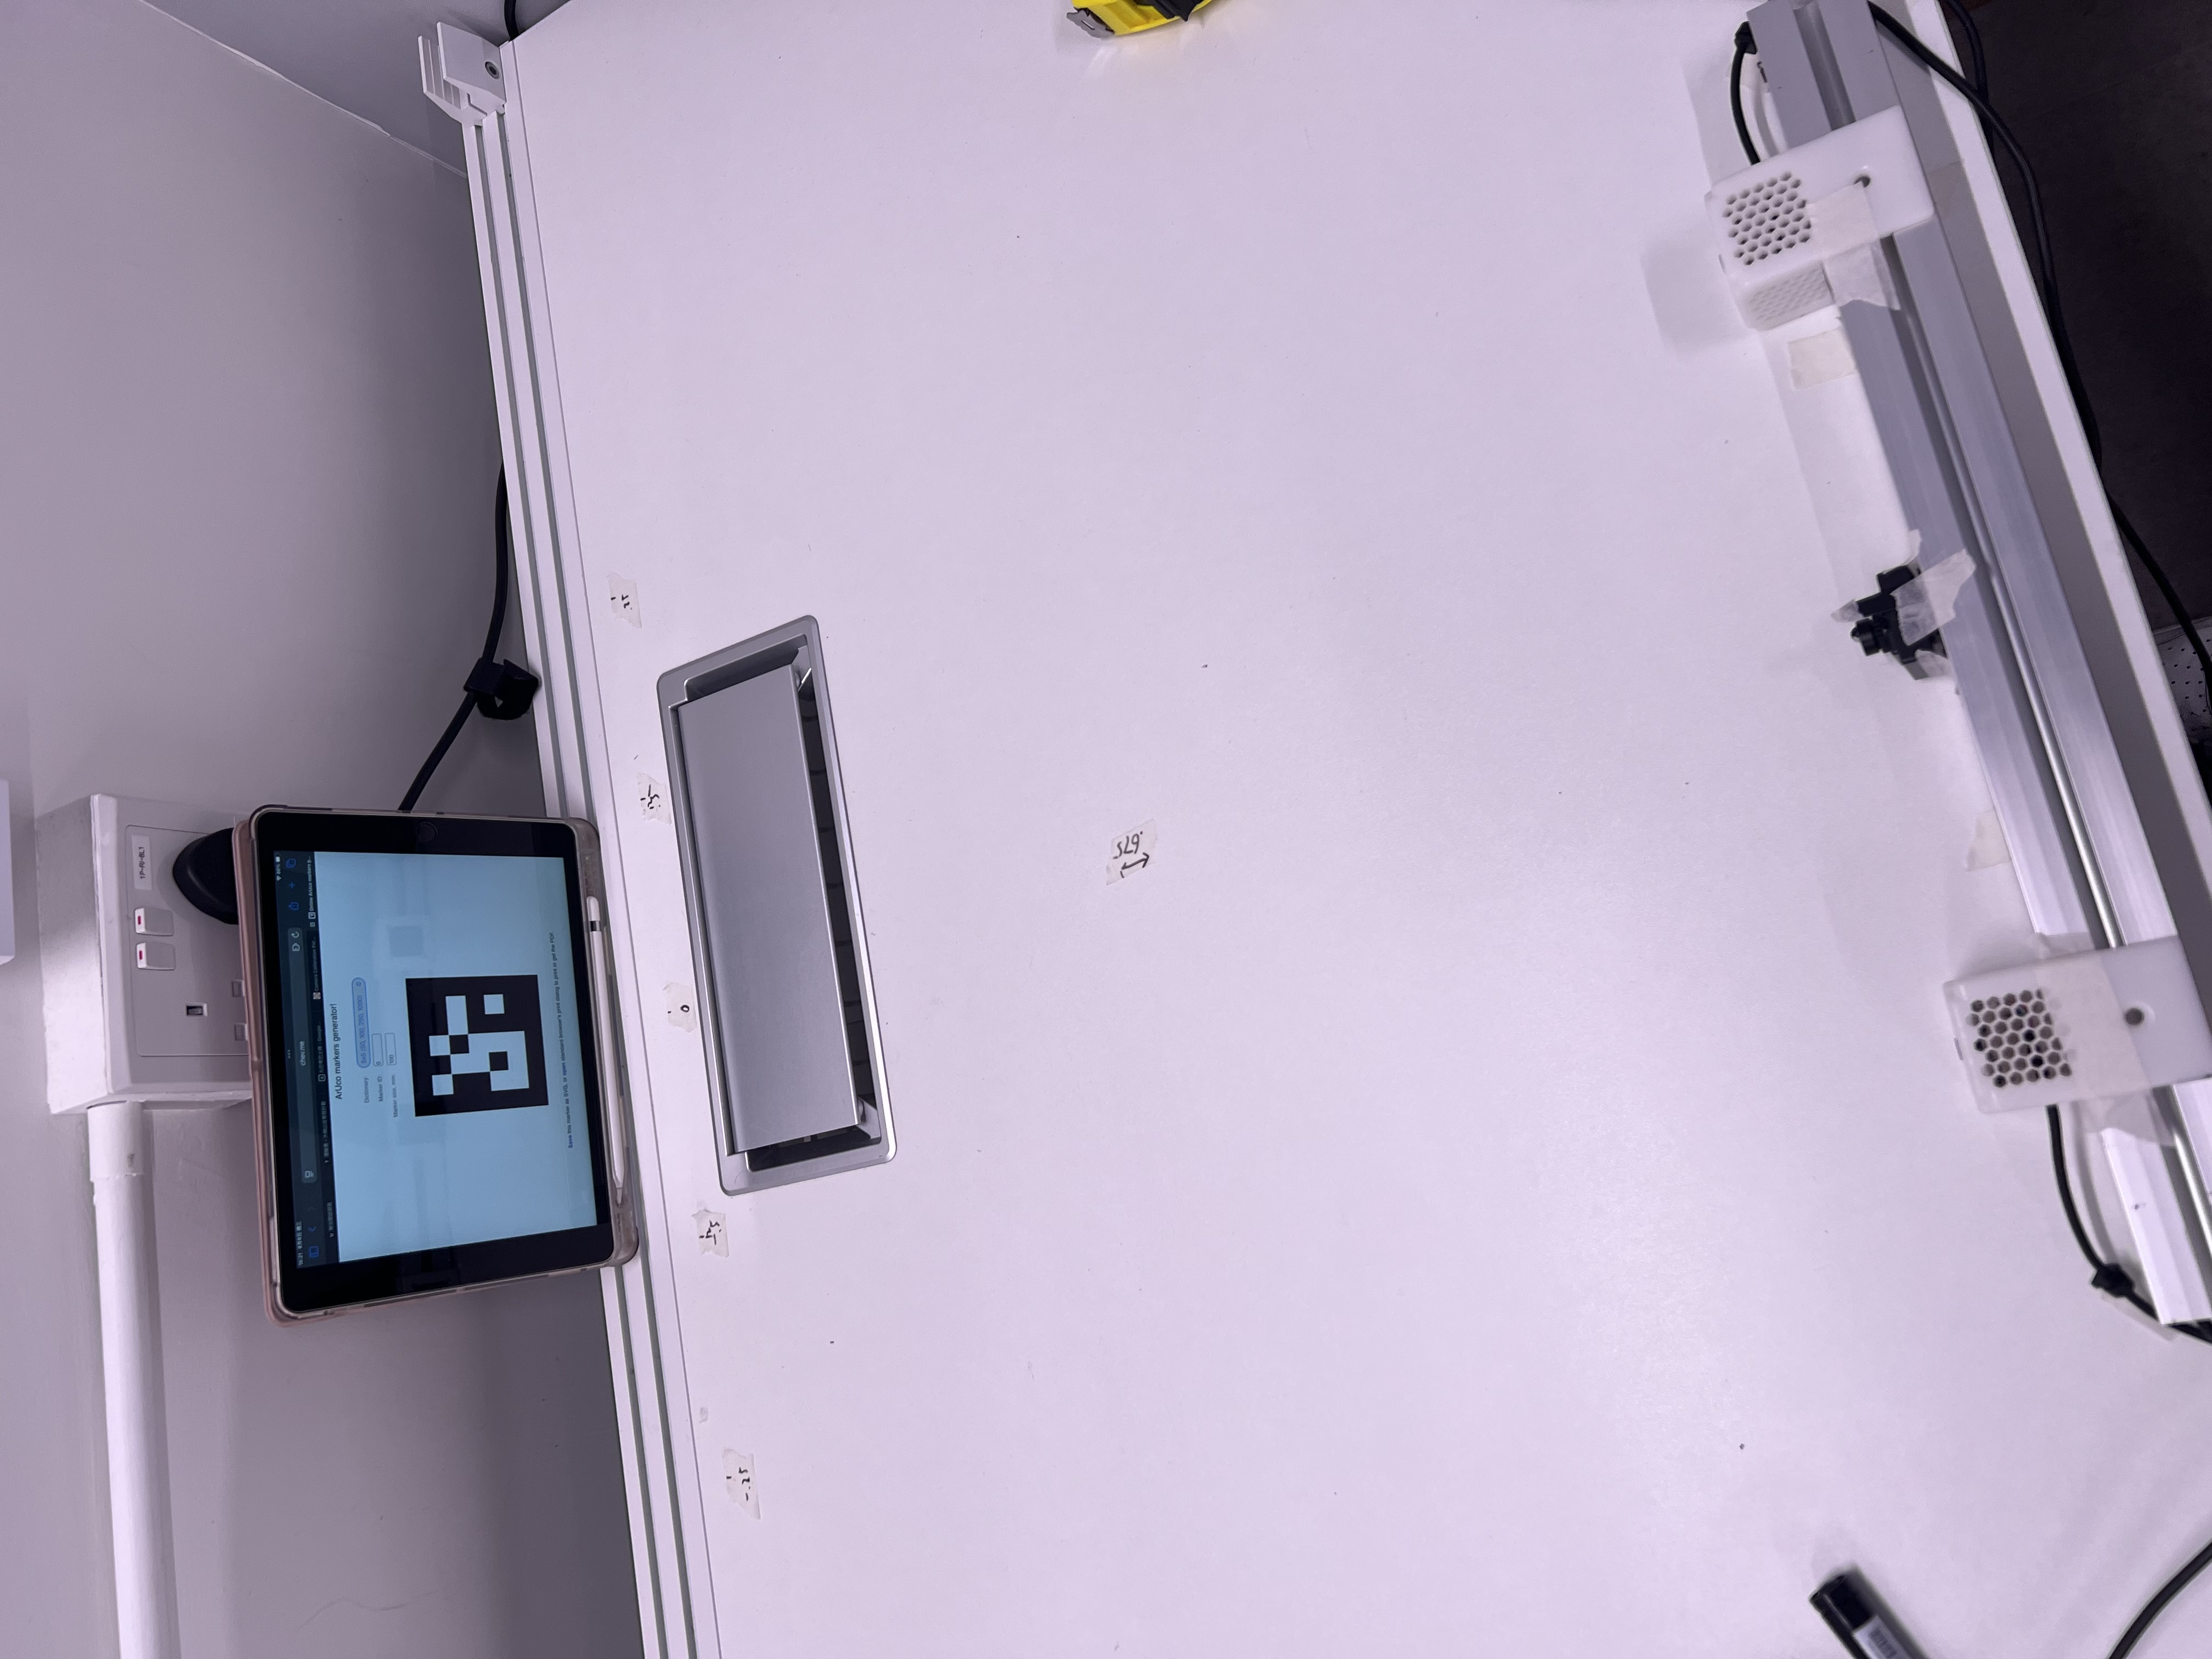
\includegraphics[width=0.6\linewidth]{figures/aruco test.jpeg}
                }
                    \caption{ArUco marker tracking test setup showing marker movement along a linear path. The coordinate axes overlaid on the marker demonstrate successful pose estimation, with position data collected at 0.125m intervals for localization accuracy validation.}
                    \label{aruco test}
            \end{figure}

            
            \item \textbf{Task 3.2: Multi-Camera Fusion}\\\\
            \textbf{Aim:} Combine detections of the ArUco markers from multiple cameras.\\
            \textbf{Expected Outcome:} The ArUco markers can be located according to detections from multiple cameras.\\
            \textbf{Group member in charge:} XU, Borong\\
            \textbf{Work:} We wrote an algorithm to combine detections from multiple cameras. Weighted averaging was implemented based on detection confidence and viewing angle. The algorithm also handles occlusions and marker visibility transitions between cameras by estimating the AUV's position from previous frames.\\\\


            \begin{figure}
                    \centering
                    \rotatebox{0}{
                    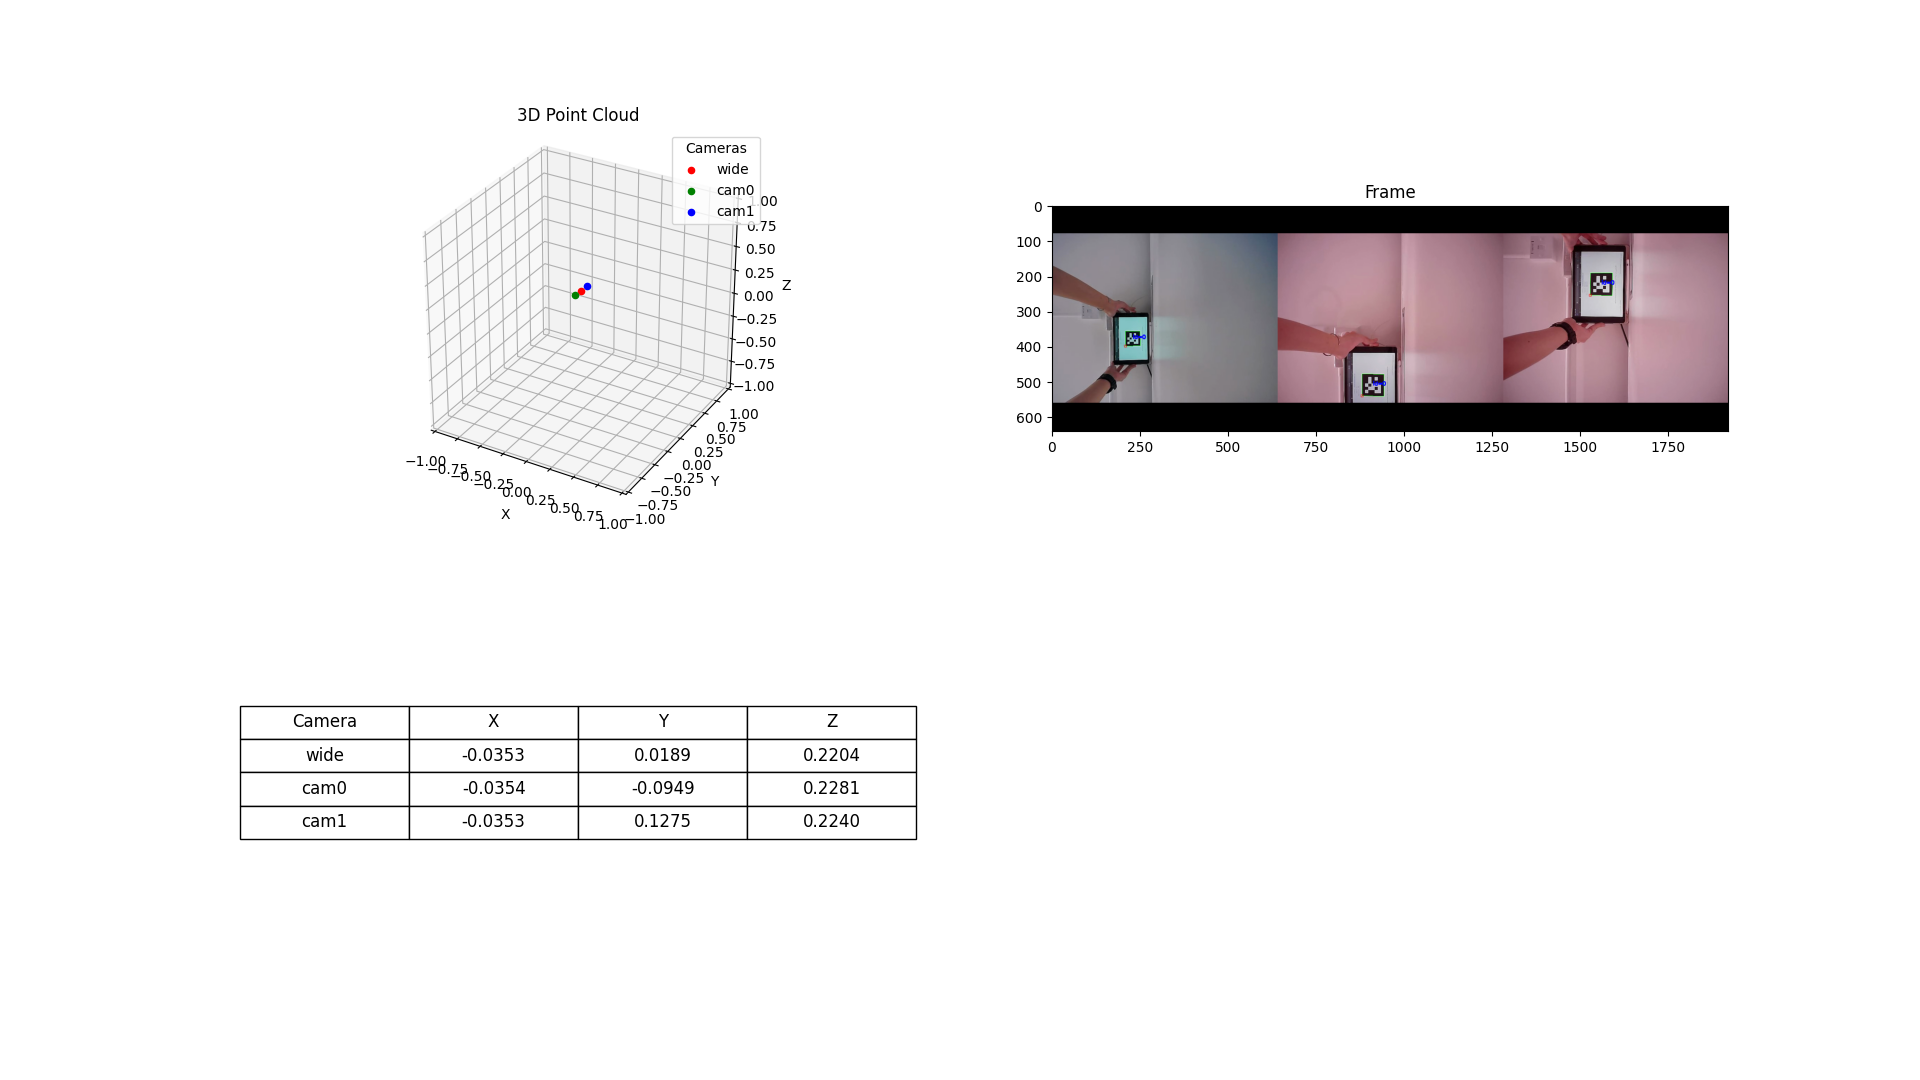
\includegraphics[width=0.6\linewidth]{figures/share_local.png}
                    }
                    \caption{Comparison of localization results from multiple cameras viewing the same ArUco marker. The scatter plot shows position estimates in the xy-plane, highlighting inconsistencies between camera coordinate systems before extrinsic calibration and fusion.}
                    \label{share_local}
                \end{figure}
            \begin{figure}
                    \centering
                    \rotatebox{0}{
                    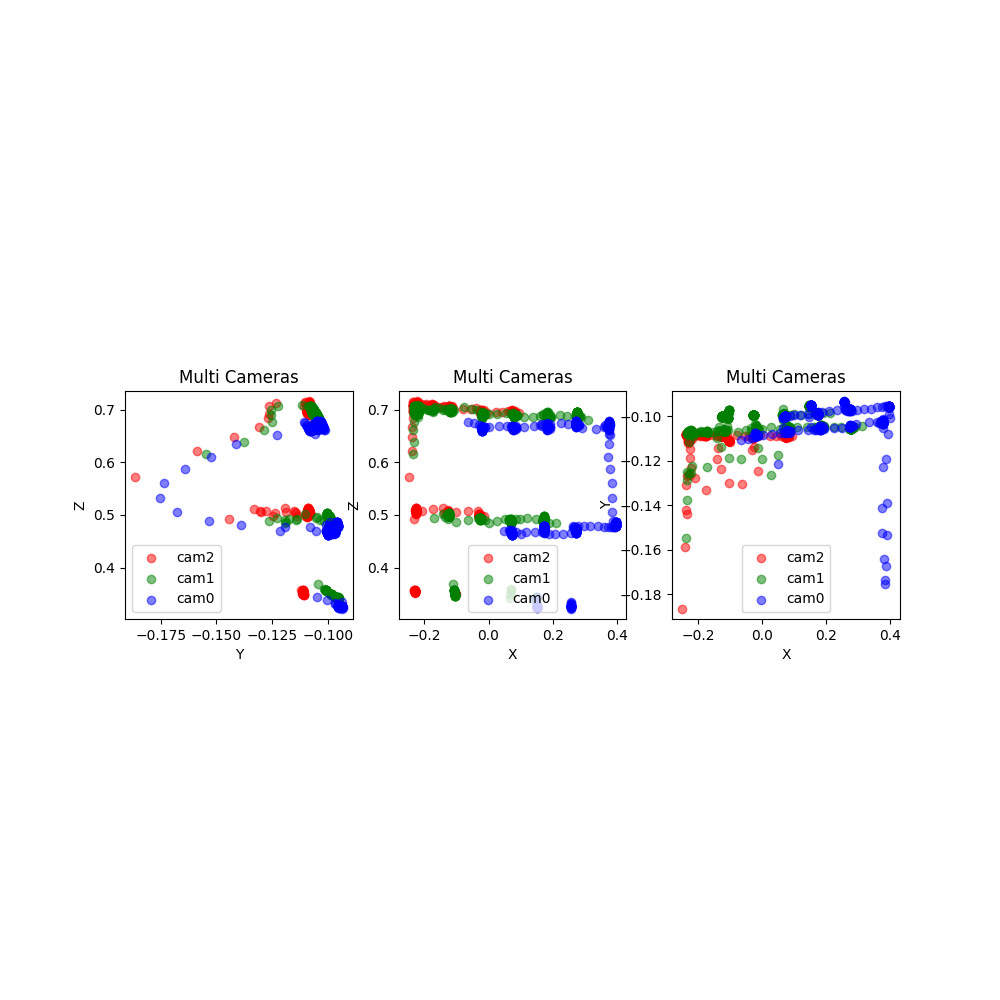
\includegraphics[width=0.6\linewidth]{figures/air_tracking.png}
                    }
                    \caption{ArUco marker trajectory tracking in air showing consistent localization performance. The smooth path (blue line) with minimal scatter demonstrates accurate pose estimation without refractive distortion effects.}
                    \label{air_tracking}
            \end{figure}
            \begin{figure}
                    \centering
                    \rotatebox{0}{
                    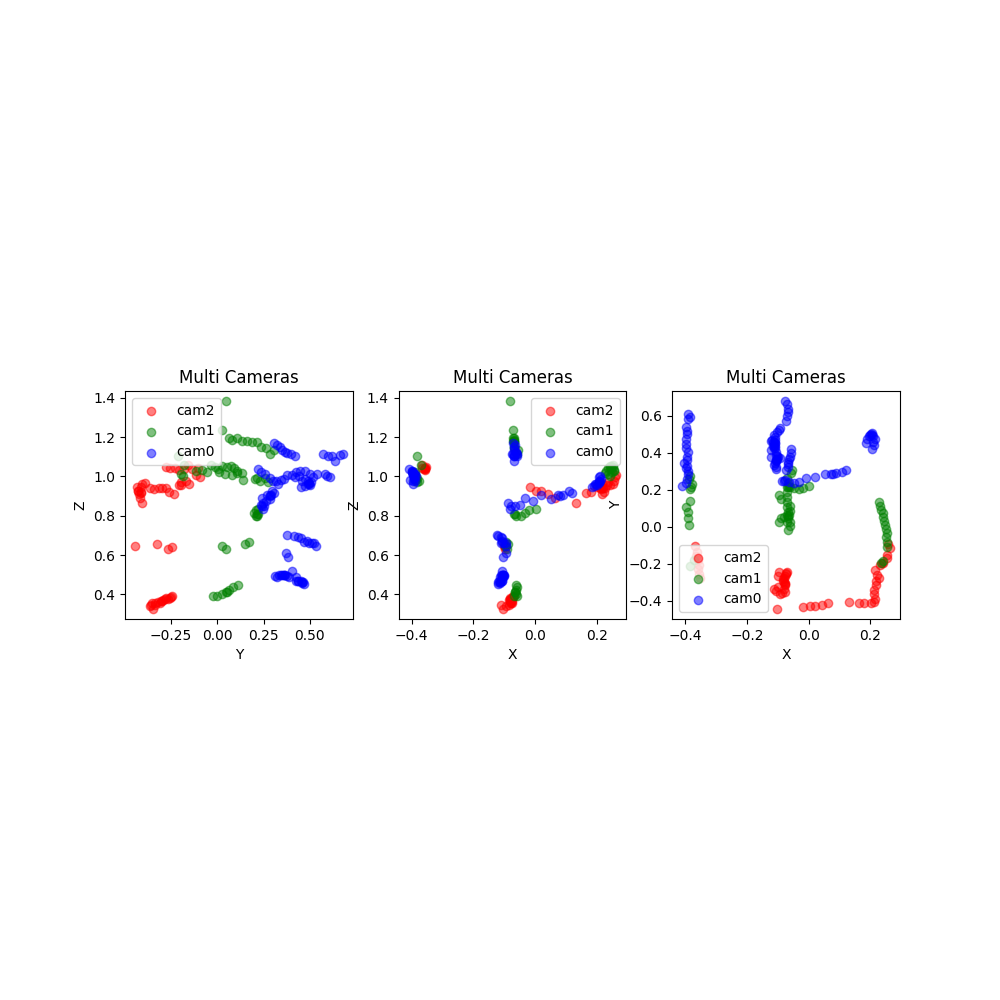
\includegraphics[width=0.6\linewidth]{figures/water_tracking.png}
                    }
                    \caption{ArUco marker trajectory tracking underwater with the same distortion parameter in air. Showing increased localization variability due to refraction effects. The scattered position estimates highlight the need for refraction-corrected calibration parameters and robust multi-camera fusion algorithms.}
                    \label{water_tracking}
            \end{figure}
            
            % \item \textbf{Task 3.3: AUV localization and results validation}\\\\
            % \textbf{Aim:} Get locations of AUVs and validate the results.\\
            % \textbf{Expected Outcome:} Localize at least 3 AUVs with positional accuracy within $\pm 7\times 10^ {- 2} $ m and achieve a detection speed of at least 10Hz.\\
            % \textbf{Group member in charge:} Both members\\
            % \textbf{Work:} Yet to start: Depending on Tasks 3.2.

        \end{itemize}

        \subsubsection{Objective Statement 4: RSSI localization Implementation}
        The objective is to utilize RSSI localization to get the coordinates of the AUVs for comparing with the results from optical localization.

        \textbf{Tasks:}
        \begin{itemize}
            \item \textbf{Task 4.1: RSSI Calibration}\\\\
            \textbf{Aim:} Map the received signal strength to the distance between the RSSI sensor and the target device.\\
            \textbf{Expected Outcome:} Error has to be within $7.0\times10^{-2}$m.\\
            \textbf{Group member in charge:} CHAN, Sze Sen\\
            \textbf{Work:} We wrote an algorithm in Arduino IDE to get the received signal strength from the target device using an ESP32 Devkit S3 module board. In the experiment, the distance between the board and the target device is measured, and the algorithm records the mean signal strength at certain distances. \\\\

            \item \textbf{Task 4.2: AUV localization with RSSI}\\\\
            \textbf{Aim:} Get locations of AUVs by RSSI localization.\\
            \textbf{Expected Outcome:} Localize at least 3 AUVs with positional accuracy within $\pm 7\times 10^ {- 2} $ m and achieve a detection speed of at least 10Hz.\\
            \textbf{Group member in charge:} CHAN, Sze Sen\\
            \textbf{Work:} \\\\
        \end{itemize}

        % \subsubsection{Objective Statement 5: Sensor Fusion Implementation}
        % The objective is to utilize a sensor fusion algorithm to combine the results from different cameras and RSSI localization.
        
        % \textbf{Tasks:}
        % \begin{itemize}
        %     \item \textbf{Task 5.1: Extended Kalman Filter Implementation}\\\\
        %     \textbf{Aim:} Implement the Extended Kalman Filter to combine the results of different cameras and RSSI localization.\\
        %     \textbf{Expected Outcome:} All results are well combined.\\
        %     \textbf{Group member in charge:} XU, Borong\\
        %     \textbf{Work:} Yet to start: Depending on Tasks 3.
        %     %\begin{itemize}
        %     %    \item Group member in charge: XU, Borong
        %     %    \item Task description: Design and implement an Extended Kalman Filter for asynchronous sensor fusion. Calculate the AUV velocity based on the camera-based localization. Combine vision-based position estimates from different cameras in a prediction-update framework. Tune filter parameters for optimal performance.
        %     %    \item Yet to start: Depending on Tasks 1.3, 3.3.
        %     %\end{itemize}
        % \end{itemize}

    \subsection{Main Objective Evaluation \& Discussion}

\section{Conclusion}
\TODO{}

% References
\newpage
\addcontentsline{toc}{section}{References}
    \bibliographystyle{IEEEtran}
    \bibliography{Bib}

% Appendices
\newpage
\section*{Appendices}
\addcontentsline{toc}{section}{Appendices}
    \subsection*{Appendix A - Project Schedule} 
    \addcontentsline{toc}{subsection}{Appendix A - Project Schedule}
        \newpage
        \centering
        \begin{adjustbox}{max width=\textheight, angle=90}
        \begin{tabular}{|p{3cm}|p{3cm}|p{1.5cm}|p{0.75cm}|p{0.75cm}|p{0.75cm}|p{0.75cm}|p{0.75cm}|p{0.75cm}|p{0.75cm}|p{0.75cm}|p{0.75cm}|p{0.9cm}|p{0.9cm}|p{0.9cm}|p{0.9cm}|p{0.9cm}|p{0.9cm}|p{0.9cm}|p{0.9cm}|}
        \hline
        Objective statements& Task & Group Member in charge & WK1 28/7 & WK2 4/8 & WK3 11/8 & WK4 18/8 & WK5 25/8 & WK6 1/9 & WK7 8/9 & WK8 15/9 & WK9 22/9 & WK10 29/9 & WK11 6/10 & WK12 13/10 & WK13 20/10 & WK14 27/10 & WK15 3/11 & WK16 10/11 & WK17 17/11 \\
        \hline
         Simulation Environment Development&&&\cellcolor{blue!20}&\cellcolor{blue!20}&  &  &  &  &  &  &  &  &  &  &  &\cellcolor{blue!20}&\cellcolor{blue!20}&\cellcolor{blue!20}&\cellcolor{blue!20}\\
        \hline
         &Simulation Framework Setup  &XU, Borong&\cellcolor{yellow!20}&\cellcolor{yellow!20}&  &  &  &  &  &  &  &  &  &  &  &\cellcolor{yellow!20}&\cellcolor{yellow!20}&  &  \\
        \hline
         &Noise Modeling Implementation  &XU, Borong&  &  &  &  &  &  &  &  &  &  &  &  &  &\cellcolor{yellow!20}&\cellcolor{yellow!20}&&  \\
        \hline
         &Validation and Testing of algorithms&XU, Borong&  &  &  &  & &  &  &  &  &  &  &  &  &\cellcolor{yellow!20}&\cellcolor{yellow!20}&\cellcolor{yellow!20}&\cellcolor{yellow!20}\\
        \hline
         Camera Array Calibration&  &  &  &\cellcolor{blue!20}&\cellcolor{blue!20}&\cellcolor{blue!20}&\cellcolor{blue!20}&\cellcolor{blue!20}&\cellcolor{blue!20}&\cellcolor{blue!20}&\cellcolor{blue!20}&\cellcolor{blue!20}&\cellcolor{blue!20}&\cellcolor{blue!20}&\cellcolor{blue!20}&\cellcolor{blue!20}&\cellcolor{blue!20}&\cellcolor{blue!20}&\cellcolor{blue!20}\\
        \hline
         & Chessboard photo collection&CHAN, Sze Sen&  &\cellcolor{yellow!20}&\cellcolor{yellow!20}&&&&  &  &  &  &\cellcolor{yellow!20}&\cellcolor{yellow!20}&  &  &  &  &  \\
        \hline
         &Intrinsic Parameter Calibration&Both&  &  &\cellcolor{yellow!20}&\cellcolor{yellow!20}&\cellcolor{yellow!20}&\cellcolor{yellow!20}&&&&  &  &\cellcolor{yellow!20}&\cellcolor{yellow!20}&  &  &  &  \\
        \hline
         &Extrinsic Parameter Calibration&Both&  &  &  &  &  &\cellcolor{yellow!20}&\cellcolor{yellow!20}&\cellcolor{yellow!20}&  &  &  &  &\cellcolor{yellow!20}&\cellcolor{yellow!20}&  &  &  \\
        \hline
         &Underwater Calibration Adjustment&Both&  &  &  &  &  &  &  &  &\cellcolor{yellow!20}&\cellcolor{yellow!20}&  &  &  &  &\cellcolor{yellow!20}&\cellcolor{yellow!20}&\cellcolor{yellow!20}\\
         \hline
         ArUco Tracking Implementation&  &  &  &  &\cellcolor{blue!20}&\cellcolor{blue!20}&\cellcolor{blue!20}&\cellcolor{blue!20}&  &  &  &\cellcolor{blue!20}&\cellcolor{blue!20}&\cellcolor{blue!20}&\cellcolor{blue!20}&\cellcolor{blue!20}&\cellcolor{blue!20}&\cellcolor{blue!20}&\cellcolor{blue!20} \\
         \hline
         & ArUco Localization Algorithm&Both&  &  &\cellcolor{yellow!20}&\cellcolor{yellow!20}&\cellcolor{yellow!20}&\cellcolor{yellow!20}&  &  &  &\cellcolor{yellow!20}&\cellcolor{yellow!20}&  &  &  &  &  &  \\
         \hline
         &Multi-Camera Fusion&XU, Borong&  &  &  &  &  &  &  &  &  &  &\cellcolor{yellow!20}&\cellcolor{yellow!20}&\cellcolor{yellow!20}&\cellcolor{yellow!20}&  &  &  \\
         \hline
         &AUV localization and results validation&Both&  &  &  &  &  &  &  &  &  &  &  &  &  &  &\cellcolor{yellow!20}&\cellcolor{yellow!20}&\cellcolor{yellow!20}\\
         \hline
         Sensor Fusion Implementation&  &  &  &  &  &  &  &  &  &  &  &  & &\cellcolor{blue!20}&\cellcolor{blue!20}&\cellcolor{blue!20}&\cellcolor{blue!20}&\cellcolor{blue!20}&\cellcolor{blue!20}\\
         \hline
         &Extended Kalman Filter Implementation&XU, Borong&  &  &  &  &  &  &  &  &  &  &  &\cellcolor{yellow!20}&\cellcolor{yellow!20}&\cellcolor{yellow!20}&\cellcolor{yellow!20}&\cellcolor{yellow!20}&\cellcolor{yellow!20}\\
        \hline
        \end{tabular}
        \end{adjustbox}
        \label{tab:placeholder}
    \subsection*{Appendix B - Budget} 
    \addcontentsline{toc}{subsection}{Appendix B - Budget}
        \begin{longtable}[c]{| l | c | c |}
            \caption{List of budget\label{budget}}\\ 
            \hline
            \textbf{Items} & \textbf{Quantity} & \textbf{Cost per each (RMB\textyen)}\\
            \hline
            WXSJ-H65HD V01 camera & 4 & \textyen 112\\
            \hline
            S-YUE 7730V1 camera & 1 & \textyen 108\\
            \hline
            UGREEN CM475 USB-C adapter & 1 & \textyen 169\\
            \hline
            3D printed Camera holder & 4 & \textyen 0*\\
            \hline
            ESP32-S3-WROOM-1 module board & 1 & \textyen 0*\\
            \hline
            3D printed ESP32 holder & 1 & \textyen 0*\\
            \hline
            M8 Screws 5pc & 4 & \textyen 2.19\\
            \hline
            M8 T-Nut 10pc & 2 & \textyen 1.6\\
            \hline
            M3 Screws and nuts 50pc & 1 & \textyen 2.77\\
            \hline
            Aluminum extrusions 2020 1000mm& 10 & \textyen 38.75\\
            \hline
            Aluminum extrusions 4040 1000mm& 10 & \textyen 62.75\\
            \hline
            Calibration boards & 5 & \textyen 0*\\
            \hline
            \textbf{Contingency Budget (15\%)} & & \textyen 212.81\\
            \hline
            \textbf{Total (including contingency)} & & \textyen 1631.54\\
            \hline
        \end{longtable}

        \textbf{Budget Justification:}
        \begin{itemize}
            \item \textbf{No-cost items (*):} 3D printed camera holders and calibration boards are provided by HKUST's Center for Engineering Education and Research Innovation (CEERI) through existing laboratory resources. This allocation supports academic research initiatives without additional expenditure, enabling access to professional-grade prototyping facilities.
            \item \textbf{Camera selection:} Five cameras (4× WXSJ-H65HD + 1× S-YUE) provide optimal cost-performance ratio at ¥110/camera average, offering 1280×960 resolution with OpenCV compatibility for real-time processing at 10 Hz.
            \item \textbf{Contingency allocation:} 15\% contingency (¥212.81) covers potential hardware failures, additional calibration materials, or unexpected software licensing costs, ensuring project completion within budget constraints.
            \item \textbf{Cost optimization:} Total budget of ¥1418.73 represents significant savings compared to commercial AUV localization systems (typically ¥10,000+), achieving research-grade precision at educational price points while maintaining scalability for future multi-AUV experiments.
        \end{itemize}
    \newpage
    \subsection*{Appendix C - Meeting minutes}
    \addcontentsline{toc}{subsection}{Appendix C - Meeting minutes}
    % fake minutes summarising what we're gonna do 
    \paragraph{Meeting 1}
    \begin{itemize}
        \item Date: 8/7/2025
        \item Time: 18:00
        \item Location: Zoom meeting
        \item Attendees: CHAN, Sze Sen, XU, Borong
        \item Absent: None
        \item Minutes taken by: CHAN, Sze Sen
        \begin{itemize}
            \item Prof. Huan YIN introduces the background information of this project 
            \item We start planning the main objectives
            \item Prof. YIN also states some goals we have to achieve, and can challenge
            \item Primary Goals:
            \begin{itemize}
                \item Find the x-y coordinates of AUV
                \item Find the z coordinates of AUV
                \item Find the velocity of the AUV
            \end{itemize}
            \item Challenges:
            \begin{itemize}
                \item Solve the location shift between cameras during localization
                \item Localize the AUV with a single camera
                \item Scan the AUV when part of the ArUco tag has been blocked
            \end{itemize}
        \end{itemize}
    \end{itemize}
    \begin{longtable}[c]{| l | l | l |}
        \caption{Action Items for Next Meeting\label{next meeting 1}}\\ 
        \hline
        \textbf{Action Item to be completed} & \textbf{By when} & \textbf{By whom}\\
        \hline
        Visit CKSRI for setup inspection & 13/7 & CHAN, Sze Sen\\
        \hline
        Simulation Framework Setup & 31/7 & XU, Borong\\
        \hline
        Literature reviews on different localization methods & 31/7 & All\\
        \hline
    \end{longtable}
    \begin{itemize}
        \item Next Meeting: 5/8/2025, 19:30, Zoom meeting
    \end{itemize}
    \newpage
    \paragraph{Meeting 2}
    \begin{itemize}
        \item Date: 5/8/2025
        \item Time: 19:30
        \item Location: Zoom meeting
        \item Attendees: CHAN, Sze Sen, XU, Borong
        \item Absent: None
        \item Minutes taken by: CHAN, Sze Sen
        \begin{itemize}
            \item We come up with all the main objectives of the project
            \item We all agree to use 5 cameras for localization, and to try applying IMU odometry as a challenge part later for the project
            \item We plan the experiment of camera calibration and ArUco markers localization
            \item The experiment will be held on 6/8 and 14/8, CHAN, Sze Sen will go to CKSRI for the hardware part, while XU, Borong will work on the software part online
            \item Prof. YIN suggests the settings for capturing images of ArUco markers localization
        \end{itemize}
    \end{itemize}
    \begin{longtable}[c]{| l | l | l | l |}
        \caption{Action Items from the Previous Meeting\label{previous meeting 2}}\\ 
        \hline
        \textbf{Action Item to be completed} & \textbf{By when} & \textbf{By whom} & \textbf{Status}\\
        \hline
        Visit CKSRI for setup inspection & 13/7 & CHAN, Sze Sen & Completed\\
        \hline
        Simulation Framework Setup & 31/7 & XU, Borong & Completed\\
        \hline
        Literature reviews on other localization methods & 31/7 & All & Completed\\
        \hline
    \end{longtable}
    \begin{longtable}[c]{| l | l | l |}
        \caption{Action Items for Next Meeting\label{next meeting 2}}\\ 
        \hline
        \textbf{Action Item to be completed} & \textbf{By when} & \textbf{By whom}\\
        \hline
        Image collection & 14/8 & CHAN, Sze Sen\\
        \hline
        Algorithms for intrinsic and extrinsic calibrations & 14/8 & XU, Borong\\
        \hline
        ArUco localization algorithm & 22/8 & All\\
        \hline
    \end{longtable}
    \begin{itemize}
        \item Next Meeting: 2/9/2025, 14:30, HKUST CKSRI
    \end{itemize}
    \newpage
    \paragraph{Meeting 3}
    \begin{itemize}
        \item Date: 2/9/2025
        \item Time: 14:30
        \item Location: HKUST CKSRI
        \item Attendees: CHAN, Sze Sen, XU, Borong
        \item Absent: None
        \item Minutes taken by: CHAN, Sze Sen
        \begin{itemize}
            \item The errors of intrinsic and extrinsic calibrations are $\pm 7.1\times 10^ {- 2} $ m and $\pm 2.2\times 10^ {- 2} $ m
            \item Prof. YIN suggests reduce the errors within $\pm2\times 10^ {- 2} $ m
            \item We plan to continue the lab experiment after finishing the proposal report
            \item Prof. YIN also suggests several papers that could be referred to in the proposal report
        \end{itemize}
    \end{itemize}
    \begin{longtable}[c]{| l | l | l | l |}
        \caption{Action Items from the Previous Meeting\label{previous meeting 3}}\\ 
        \hline
        \textbf{Action Item to be completed} & \textbf{By when} & \textbf{By whom} & \textbf{Status}\\
        \hline
        Image collection & 14/8 & CHAN, Sze Sen & Completed\\
        \hline
        Algorithms for intrinsic and extrinsic calibrations & 14/8 & XU, Borong & Completed\\
        \hline
        ArUco localization algorithm & 22/8 & All & Completed\\
        \hline
    \end{longtable}
    \begin{longtable}[c]{| l | l | l |}
        \caption{Action Items for Next Meeting\label{next meeting 3}}\\ 
        \hline
        \textbf{Action Item to be completed} & \textbf{By when} & \textbf{By whom}\\
        \hline
        Proposal Report Introduction & 26/9 & CHAN, Sze Sen\\
        \hline
        Proposal Report Methodology & 26/9 & XU, Borong\\
        \hline
        Finalize the proposal report & 29/9 & All\\
        \hline
    \end{longtable}
    \begin{itemize}
        \item Next Meeting: 8/10/2025, 14:30, HKUST CKSRI
    \end{itemize}
    \newpage
    \paragraph{Meeting 4}
    \begin{itemize}
        \item Date: 8/10/2025
        \item Time: 14:30
        \item Location: HKUST CKSRI
        \item Attendees: CHAN, Sze Sen, XU, Borong
        \item Absent: None
        \item Minutes taken by: XU, Borong
        \begin{itemize}
            \item We completed calibration of the camera's intrinsic parameters for single-camera localization in air, designing and mounting the camera array under the experimental water tank
            \item We also designed a new method for camera calibration using ChArUco boards to improve the accuracy of cross-camera views
            \item We are now facing difficulties with the theoretical model of multi-camera calibration, which requires further literature review, and the gap between in-air and underwater cross-medium environments needs validation through underwater experiments
            \item Prof. YIN provides feedback on refining the calibration approach,  suggested additional references for modeling cross-medium distortion, and also suggested implying RSSI localization as an assisting method
            \item We all agree to explore RSSI as an assisting localization method, model cross-medium light refraction, and conduct initial underwater experiments
        \end{itemize}
    \end{itemize}
    \begin{longtable}[c]{|l|l|l|l|}
        \caption{Action Items from the Previous Meeting}\\
        \hline
        \textbf{Action Item to be completed} & \textbf{By when} & \textbf{By whom} & \textbf{Status} \\
        \hline
        \endhead
        Proposal Report Introduction & 26/9 & CHAN, Sze Sen & Completed \\
        \hline
        Proposal Report Methodology & 26/9 & XU, Borong & Completed \\
        \hline
        Finalize the proposal report & 29/9 & All & Completed \\
        \hline
    \end{longtable}
    \begin{longtable}[c]{|l|l|l|}
        \caption{Action Items for Next Meeting}\\
        \hline
        \textbf{Action Item to be completed} & \textbf{By when} & \textbf{By whom} \\
        \hline
        \endhead
        Literature review on RSSI for localization & 22/10 & CHAN, Sze Sen \\
        \hline
        Develop algorithm for cross-medium light refraction modeling & 22/10 & XU, Borong \\
        \hline
        Prepare and conduct initial underwater experiments & 29/10 & All \\
        \hline
    \end{longtable}
    \begin{itemize}
        \item Next Meeting: 5/11/2025, 14:30, HKUST CKSRI
    \end{itemize}
    \newpage
    \paragraph{Meeting 5}
    \begin{itemize}
        \item Date: 5/11/2025
        \item Time: 14:30
        \item Location: HKUST CKSRI
        \item Attendees: CHAN, Sze Sen, XU, Borong
        \item Absent: None
        \item Minutes taken by: XU, Borong
        \begin{itemize}
            \item We completed calibration of the camera's intrinsic parameters for single-camera localization in both air and underwater, calibration of extrinsic parameters for the new camera array and mounting under the water tank
            \item We also developed and implemented algorithms to localize ArUco marks
            \item The literature review on the implementation of RSSI as an assisting localization method was conducted
            \item We are now facing difficulties with underwater experiments, which reveal a gap between in-air and underwater intrinsic calibration, and a suitable Python environment for the RSSI system requires further research
            \item Prof. YIN provides feedback on addressing the calibration gap through additional modeling and suggested references for RSSI implementation and Python environments
            \item We all agree to investigate RSSI implementation through further literature reviews, use mathematical models to optimize non-linear point projection from 2D to 3D, conduct more underwater experiments, and develop a Python environment showing the relationship between signal strength and AUV position
        \end{itemize}
    \end{itemize}
    
    \begin{longtable}[c]{|l|l|l|l|}
        \caption{Action Items from the Previous Meeting}\\
        \hline
        \textbf{Action Item to be completed} & \textbf{By when} & \textbf{By whom} & \textbf{Status} \\
        \hline
        \endhead
        Literature review on RSSI for localization & 22/10 & CHAN, Sze Sen & Completed \\
        \hline
        Develop algorithm for cross-medium light refraction modeling & 22/10 & XU, Borong & Completed \\
        \hline
        Prepare and conduct initial underwater experiments & 29/10 & All & Completed \\
        \hline
    \end{longtable}
    \begin{longtable}[c]{|l|l|l|}
        \caption{Action Items for Next Meeting}\\
        \hline
        \textbf{Action Item to be completed} & \textbf{By when} & \textbf{By whom} \\
        \hline
        \endhead
        Investigate implementation of RSSI through literature reviews & 20/11 & CHAN, Sze Sen \\
        \hline
        Use mathematical models to optimize non-linear point projection & 20/11 & XU, Borong \\
        \hline
        Conduct more underwater experiments to test the algorithm & 27/11 & All \\
        \hline
        Develop Python environment for signal strength and AUV position & 27/11 & All \\
        \hline
    \end{longtable}
    \begin{itemize}
    \item Next Meeting: 3/12/2025, 14:30, HKUST CKSRI
    \end{itemize}
    \newpage
    \paragraph{Meeting 6}
    \begin{itemize}
        \item Date: 3/12/2025
        \item Time: 14:30
        \item Location: HKUST CKSRI
        \item Attendees: CHAN, Sze Sen, XU, Borong
        \item Absent: None
        \item Minutes taken by: CHAN, Sze Sen
        \begin{itemize}
            \item The development of the Python environment for signal strength and AUV position is still in progress since further investigation on the module board given by Prof. YIN is required
            \item Prof. YIN mentions that he would leave HKUST, so the supervisor of this project would be changed to Prof. Fumin ZHANG
            \item We plan to continue the lab experiment after finishing the progress report and midterm poster
            \item Prof. YIN suggests that we should include more about the gaps of traditional localization methods and our plan for the remaining parts of this project in the progress report, and add more images instead of much text to draw attention in the midterm poster
        \end{itemize}
    \end{itemize}
    
    \begin{longtable}[c]{|l|l|l|l|}
        \caption{Action Items from the Previous Meeting}\\
        \hline
        \textbf{Action Item to be completed} & \textbf{By when} & \textbf{By whom} & \textbf{Status} \\
        \hline
        \endhead
        Investigate implementation of RSSI through literature reviews & 20/11 & CHAN, Sze Sen & Completed\\
        \hline
        Use mathematical models to optimize non-linear point projection & 20/11 & XU, Borong & Completed\\
        \hline
        Conduct more underwater experiments to test the algorithm & 27/11 & All & Completed\\
        \hline
        Develop Python environment for signal strength and AUV position & 27/11 & All & In progress\\
        \hline
    \end{longtable}
    \begin{longtable}[c]{|l|l|l|}
        \caption{Action Items for Next Meeting}\\
        \hline
        \textbf{Action Item to be completed} & \textbf{By when} & \textbf{By whom} \\
        \hline
        \endhead
        Progress Report Objective Statement Execution & 2/1 & CHAN, Sze Sen \\
        \hline
        Progress Report Inroduction and Methodology Overview  & 2/1 & XU, Borong \\
        \hline
        Midterm Postser & 8/1 & All \\
        \hline
        Finalize the Progress Report & 9/1 & All \\
        \hline
    \end{longtable}
    \begin{itemize}
    \item Next Meeting: 13/1/2026, 15:00, HKUST CKSRI
    \end{itemize}
    \newpage
    \paragraph{Meeting 7}
    \begin{itemize}
        \item Date: 13/1/2026
        \item Time: 15:00
        \item Location: HKUST CKSRI
        \item Attendees: CHAN, Sze Sen, XU, Borong
        \item Absent: None
        \item Minutes taken by: CHAN, Sze Sen
        \begin{itemize}
            \item We discuss our division of work for the presentation in the midterm progress day on 23/1: CHAN, Sze Sen present the overview and objectives part; XU, Borong present the methodology and progress part
            \item Prof. ZHANG suggests to use Arduino environment instead of Python for RSSI localization 
            \item We plan to test the reception of the signal strength of the ESP32 board with a simple algorithm in the Arduino environment, which only prints out the RSSI values of the target device
            \item Prof. ZHANG also suggests that we can use a device such as a phone as a target device for reception testing
        \end{itemize}
    \end{itemize}
    
    \begin{longtable}[c]{|l|l|l|l|}
        \caption{Action Items from the Previous Meeting}\\
        \hline
        \textbf{Action Item to be completed} & \textbf{By when} & \textbf{By whom} & \textbf{Status} \\
        \hline
        \endhead
        Progress Report Objective Statement Execution & 2/1 & CHAN, Sze Sen & Completed \\
        \hline
        Progress Report Inroduction and Methodology Overview  & 2/1 & XU, Borong & Completed \\
        \hline
        Midterm Postser & 8/1 & All & Completed \\
        \hline
        Finalize the Progress Report & 9/1 & All & Completed \\
        \hline
    \end{longtable}
    \begin{longtable}[c]{|l|l|l|}
        \caption{Action Items for Next Meeting}\\
        \hline
        \textbf{Action Item to be completed} & \textbf{By when} & \textbf{By whom} \\
        \hline
        \endhead
        Preparation of Midterm Progress Day & 23/1 & All \\
        \hline
        Testing of reception of the signal strength of the ESP32 board & 2/2 & XU, Borong \\
        \hline
        Develop Arduino environment for signal strength and AUV position & 11/2 & CHAN, Sze Sen \\
        \hline
    \end{longtable}
    \begin{itemize}
    \item Next Meeting: 11/2/2026, 14:00, HKUST CKSRI
    \end{itemize}
    \newpage
    \newpage
    \paragraph{Meeting 8}
    \begin{itemize}
        \item Date: 11/2/2026
        \item Time: 15:00
        \item Location: HKUST CKSRI
        \item Attendees: CHAN, Sze Sen, XU, Borong
        \item Absent: None
        \item Minutes taken by: XU, Borong
        \begin{itemize}
            \item We designed an RSSI localization method and investigated the relationship between RSSI value and the distance between the target device and signal sensor.
            \item We also investigated the calibration algorithm in OpenCV to apply the non-linear calibration.
            \item We are now facing difficulties with significant errors in distance estimation, the signal from the target device is unstable, and the OpenCV calibration algorithm requires major modification for the non-linear calibration.
            \item Prof. ZHANG provides feedback on improving RSSI data collection setup and signal stability, and suggested further detailed analysis of OpenCV non-linear calibration algorithms.
            \item We all agree to increase the amount and range of signal data collection, conduct more reviews on the causes of signal instability, perform future investigations and detailed analyses of OpenCV camera calibration algorithms, and combine the non-linear calibration algorithm with the localization algorithm.
        \end{itemize}
    \end{itemize}
    
    \begin{longtable}[c]{|l|l|l|l|}
        \caption{Action Items from the Previous Meeting}\\
        \hline
        \textbf{Action Item to be completed} & \textbf{By when} & \textbf{By whom} & \textbf{Status} \\
        \hline
        \endhead
        Preparation of Midterm Progress Day & 23/1 & All & Completed \\
        \hline
        Testing of reception of the signal strength of the ESP32 board & 2/2 & XU, Borong & Completed \\
        \hline
        Develop Arduino environment for signal strength and AUV position & 11/2 & CHAN, Sze Sen & Completed \\
        \hline
    \end{longtable}
    
    \begin{longtable}[c]{|l|l|l|}
        \caption{Action Items for Next Meeting}\\
        \hline
        \textbf{Action Item to be completed} & \textbf{By when} & \textbf{By whom} \\
        \hline
        \endhead
        Increase the amount and range of signal data collection & 25/2 & CHAN, Sze Sen \\
        \hline
        More review on the causes of signal instability & 25/2 & XU, Borong \\
        \hline
        Detailed analysis of OpenCV camera calibration algorithms & 1/3 & All \\
        \hline
        Combine the non-linear calibration algorithm with the localization algorithm & 1/3 & All \\
        \hline
    \end{longtable}
    
    \begin{itemize}
        \item Next Meeting: 24/3/2026, 16:30, HKUST CKSRI
    \end{itemize}
    \newpage
    \subsection*{Appendix D - Group Members’ Contribution}
    \addcontentsline{toc}{subsection}{Appendix D - Group Members’ Contribution}

    \paragraph{Individual Contributions:}
    \begin{itemize}
        \item \textbf{XU, Borong:} Led algorithmic development including simulation framework, camera calibration, ArUco tracking, mechanical structure design, and sensor fusion implementation. Contributed significantly to technical documentation and mathematical derivations. 
        \newpage
        \item \textbf{CHAN, Sze Sen:} 
        I was responsible for hardware integration. To do this, I visited the HKUST CKSRI lab at the beginning of the project to inspect everything initially and ensure that the five-camera array was mounted correctly under the water tank we were using for our experiment, so that the overlapping fields of view from the cameras could provide optimal coverage. 

        For Objective 1, I contributed to system specification and validation testing of the Python simulation environment for camera calibration.
    
        For Objective 2, I had to collect a large amount of data by capturing hundreds of chessboards and images in both air and underwater for camera calibration. I tried different pattern sizes and detection algorithms for the corners of these patterns to get the best results and minimize reprojection errors. For the experimental setup, I prepared and participated in initial and follow-up underwater tests, addressing challenges such as refraction distortions by validating air-water calibration gaps through hands-on trials and adjusting camera positions for better accuracy.

        For Objective 3, I also helped with validating the system by testing the ArUco marker detection in real-life scenarios. I found problems with how it worked on cameras and optimized the performance in order to achieve 10Hz detection speed.
    
        I led the documentation writing of this project. I prepared most of the meeting minutes and attached them to the report to fulfil the requirement. I prepared the introduction part of the proposal report. In this part, I stated the engineering problem of traditional localization methods. I also made literature reviews on existing solutions, including acoustic localization, magnetic localization, and optical localization. In the progress report, I added details of the objective statement execution part, including images and stating the process and challenges of the tasks. For both reports, I have to ensure that they meet all the requirements of the guidelines, and the format of writing from both members is unified. I also designed the midterm poster by including the main points of the progress report and figures we obtained during the experiment.
    
        I coordinated laboratory resources by scheduling lab access, procuring components like cameras and adapters within budget, and ensuring proper experimental procedures, such as safety protocols during water tank operations.
    
        Throughout, because of the suggestion from Prof. YIN, I conducted literature reviews on alternative localization methods, including RSSI as an assisting technique, investigating its implementation through further readings and suggesting integrations to enhance optical tracking robustness under occlusions. This practical focus complemented the algorithmic work, bridging simulation to real-world validation.
        %Managed hardware integration, data collection, and experimental setup. Led documentation efforts and contributed to system validation. Coordinated laboratory resources and ensured proper experimental procedures.
    \end{itemize}

    \newpage
    \subsection*{Appendix E - Deviation from the proposal and progress report and supporting reason}
    \addcontentsline{toc}{subsection}{Appendix E - Deviation from the proposal and progress report and supporting reason}
    \begin{flushleft} At the beginning, we try to apply optical localization only to localize the AUVs. However, once we try in the lab environment with less light, the accuracy of optical localization is limited. Therefore, we find RSSI localization as an assistant to overcome an insufficient light environment. 
    \end{flushleft}
    \newpage
    \subsection*{Appendix F - Monthly Reports}
    \addcontentsline{toc}{subsection}{Appendix F - Monthly Reports}
    \begin{figure}
        \centering
        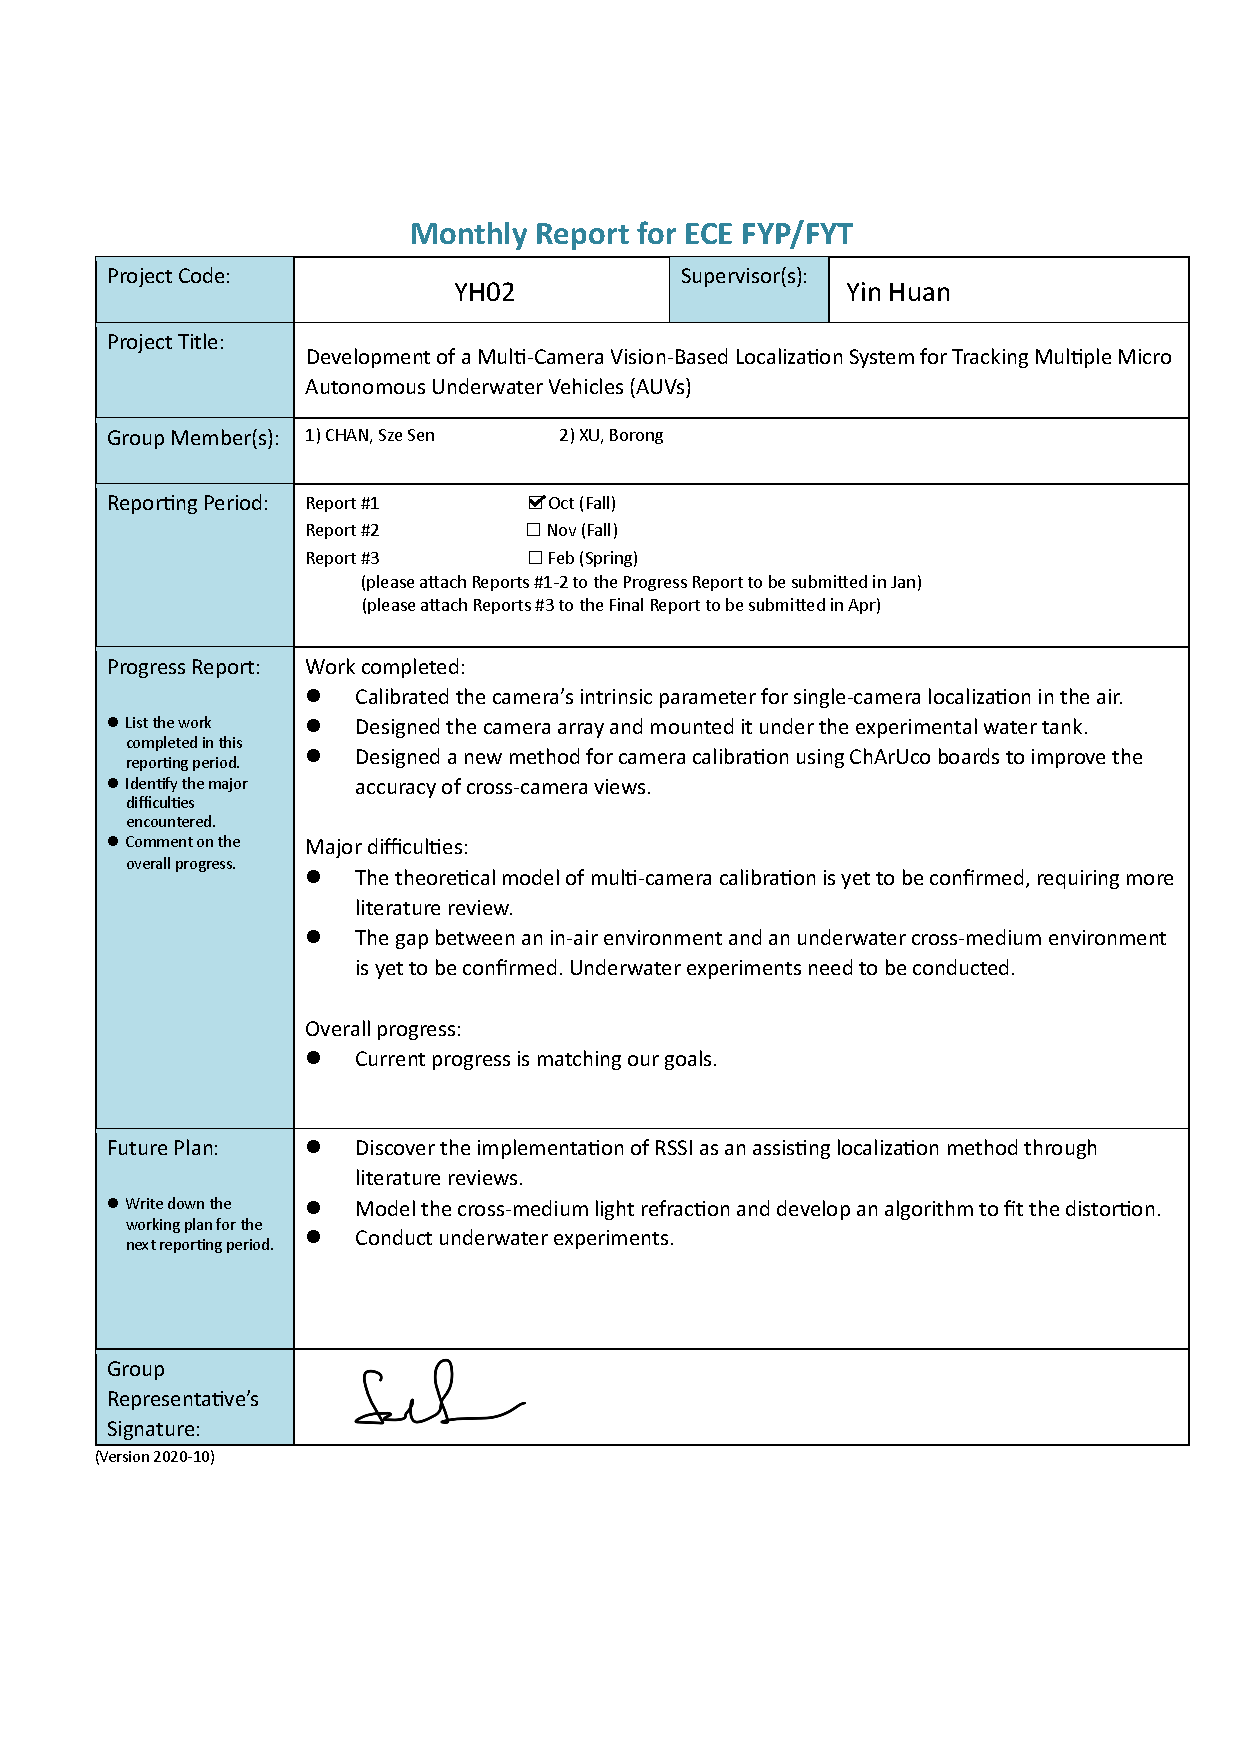
\includegraphics[width=1\linewidth]{monthly report/79_YH02a-25_MonReport1_01.pdf}
    \end{figure}
    \begin{figure}
        \centering
        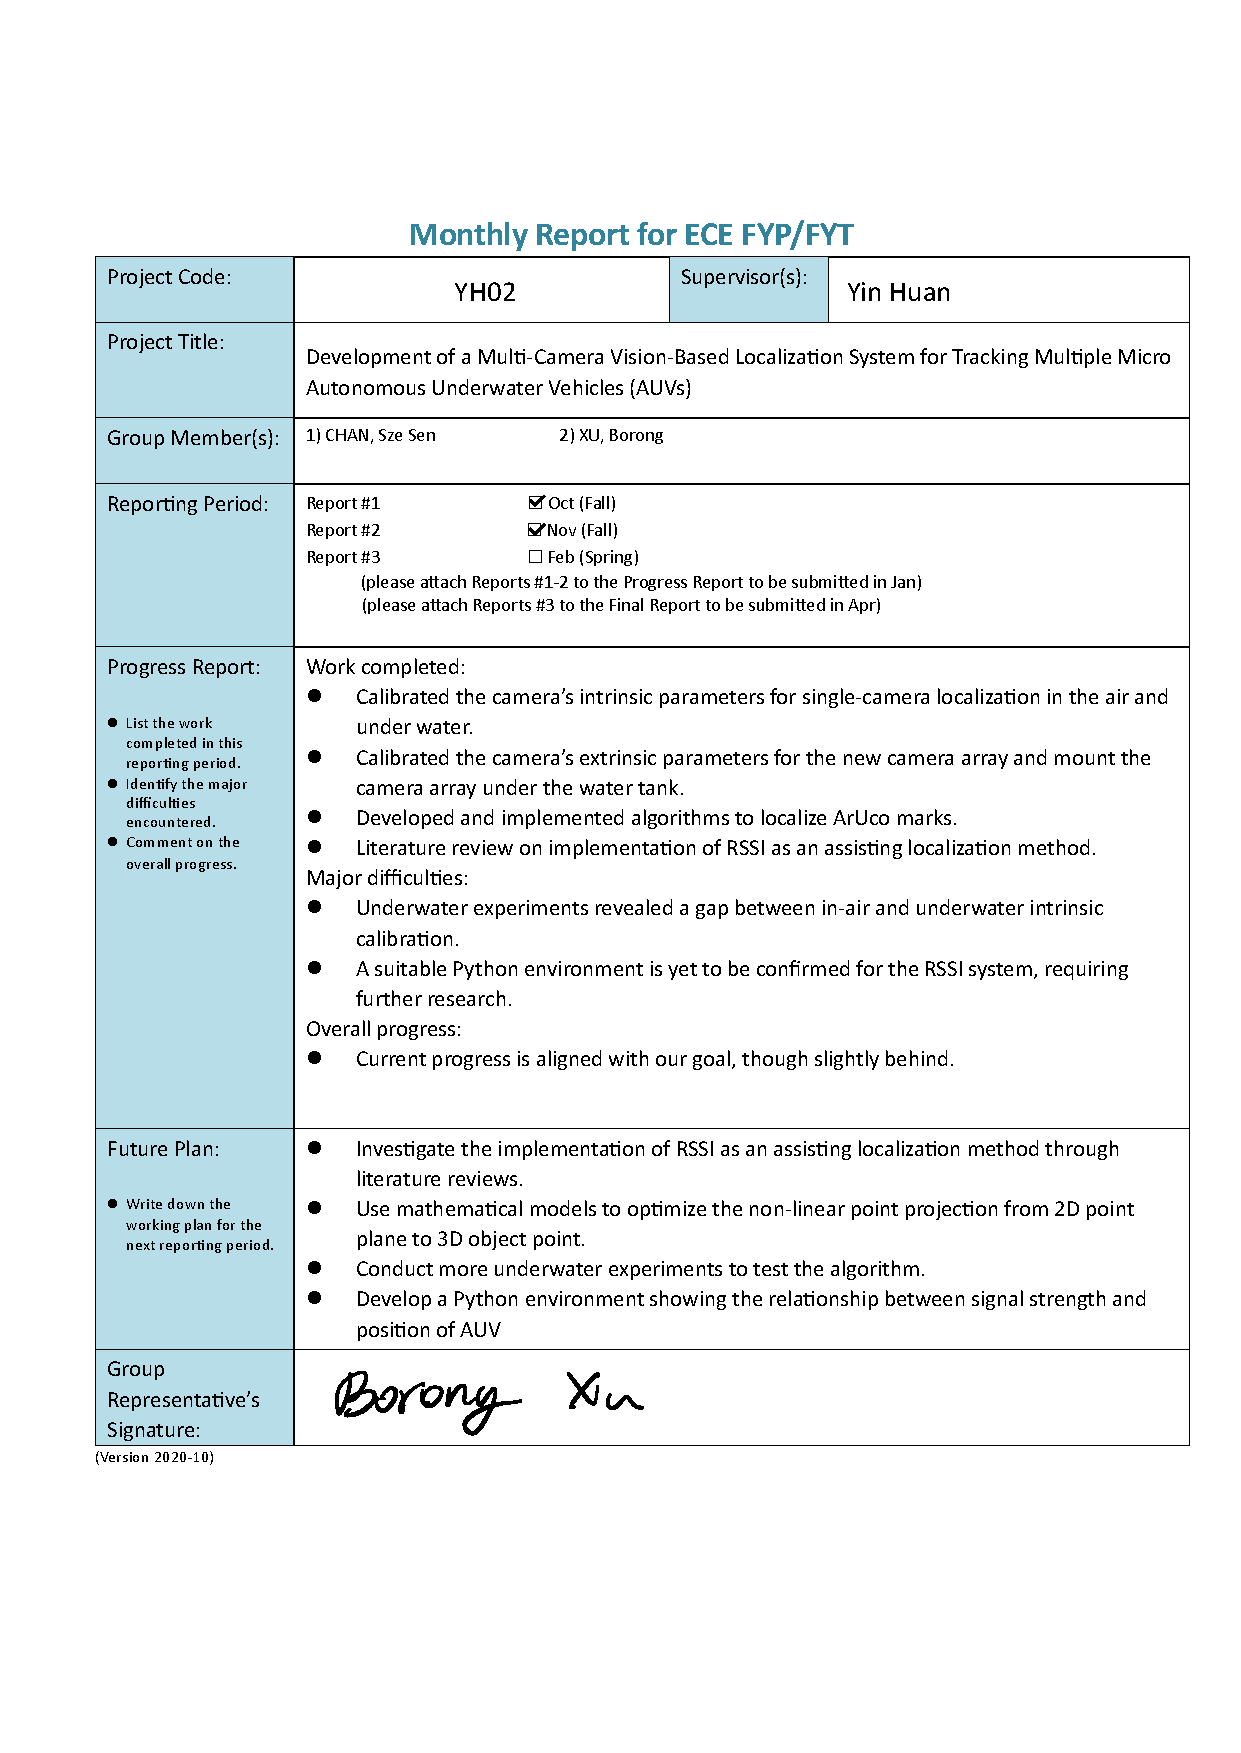
\includegraphics[width=1\linewidth]{monthly report/79_YH02a-25_MonReport2_01.pdf}
    \end{figure}
    \begin{figure}
        \centering
        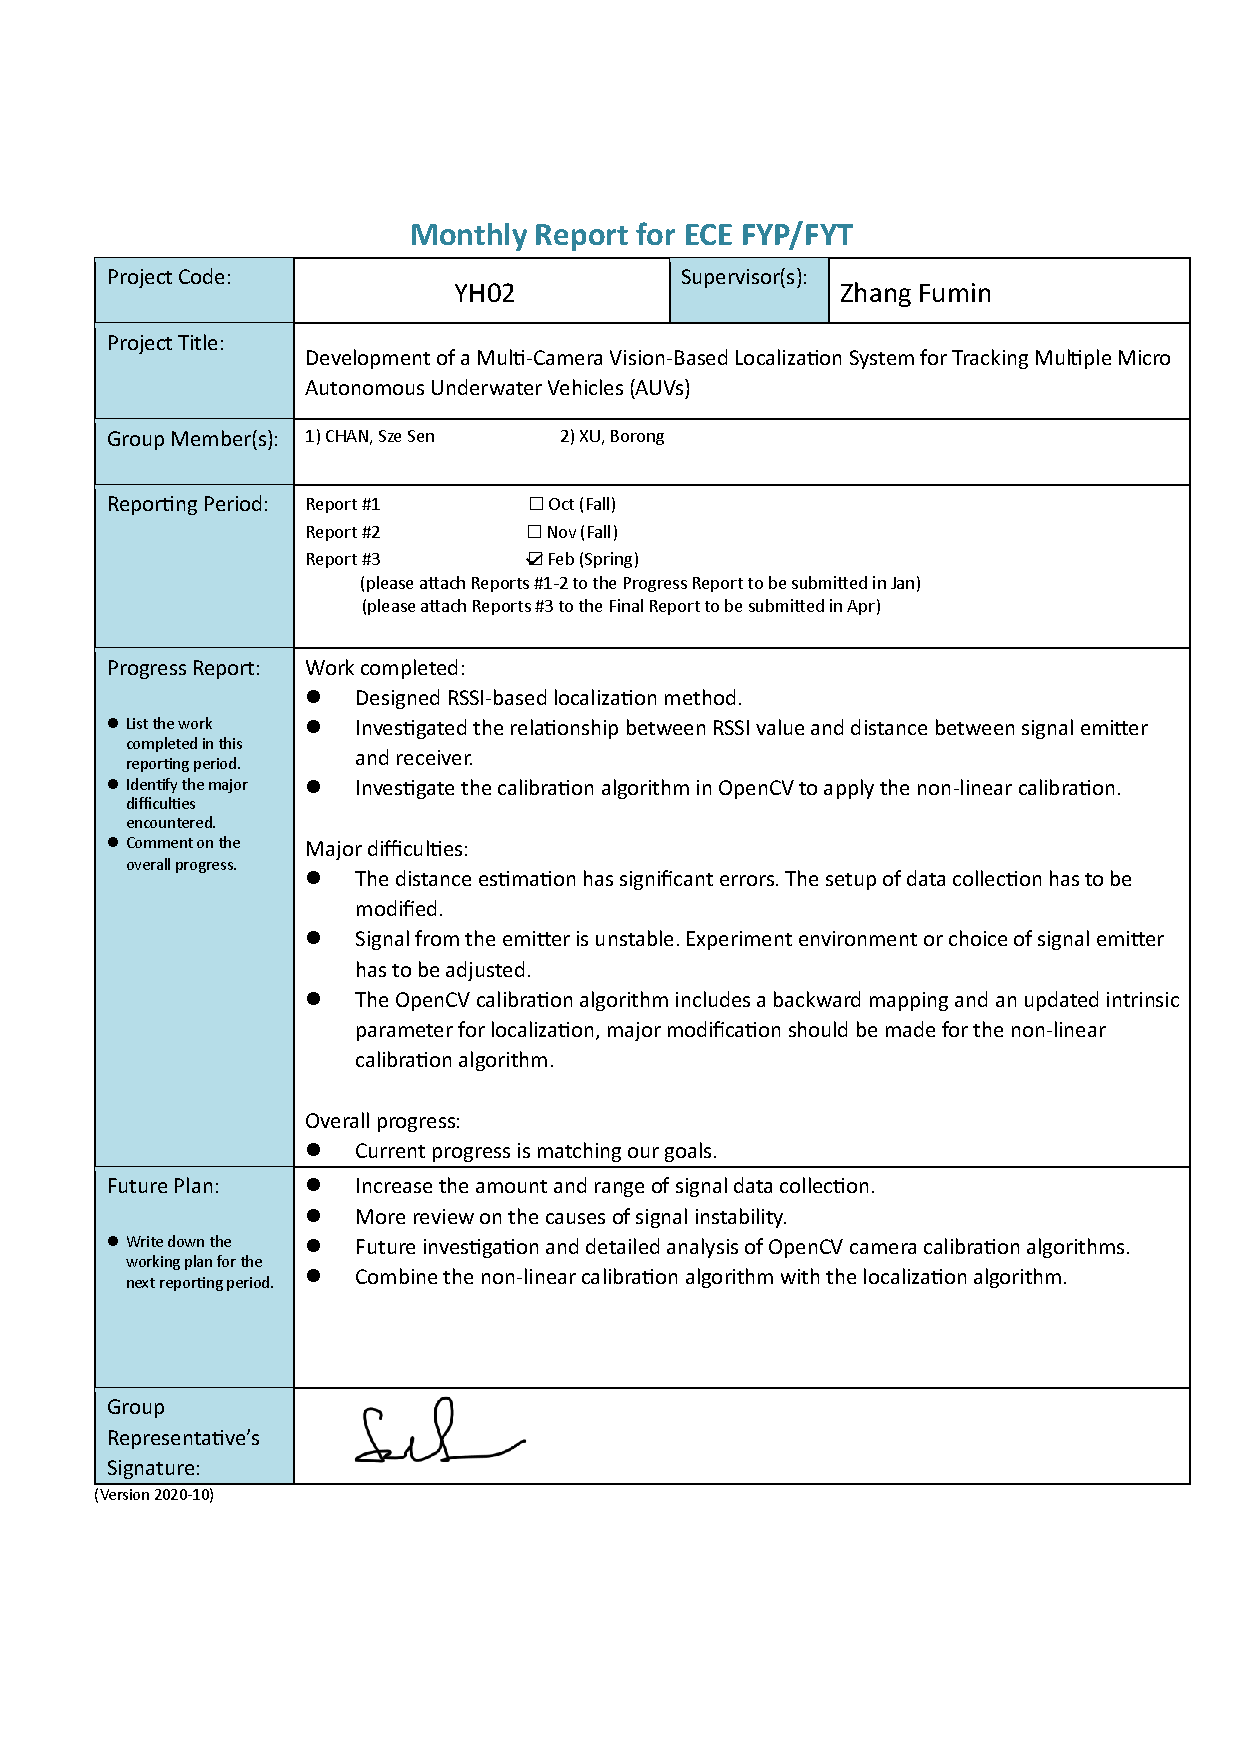
\includegraphics[width=1\linewidth]{monthly report/79_YH02a-25_MonReport3_01.pdf}
    \end{figure}    
\end{document}